\documentclass[twoside]{book}

% Packages required by doxygen
\usepackage{fixltx2e}
\usepackage{calc}
\usepackage{doxygen}
\usepackage{graphicx}
\usepackage[utf8]{inputenc}
\usepackage{makeidx}
\usepackage{multicol}
\usepackage{multirow}
\PassOptionsToPackage{warn}{textcomp}
\usepackage{textcomp}
\usepackage[nointegrals]{wasysym}
\usepackage[table]{xcolor}

% Font selection
\usepackage[T1]{fontenc}
\usepackage{mathptmx}
\usepackage[scaled=.90]{helvet}
\usepackage{courier}
\usepackage{amssymb}
\usepackage{sectsty}
\renewcommand{\familydefault}{\sfdefault}
\allsectionsfont{%
  \fontseries{bc}\selectfont%
  \color{darkgray}%
}
\renewcommand{\DoxyLabelFont}{%
  \fontseries{bc}\selectfont%
  \color{darkgray}%
}
\newcommand{\+}{\discretionary{\mbox{\scriptsize$\hookleftarrow$}}{}{}}

% Page & text layout
\usepackage{geometry}
\geometry{%
  a4paper,%
  top=2.5cm,%
  bottom=2.5cm,%
  left=2.5cm,%
  right=2.5cm%
}
\tolerance=750
\hfuzz=15pt
\hbadness=750
\setlength{\emergencystretch}{15pt}
\setlength{\parindent}{0cm}
\setlength{\parskip}{0.2cm}
\makeatletter
\renewcommand{\paragraph}{%
  \@startsection{paragraph}{4}{0ex}{-1.0ex}{1.0ex}{%
    \normalfont\normalsize\bfseries\SS@parafont%
  }%
}
\renewcommand{\subparagraph}{%
  \@startsection{subparagraph}{5}{0ex}{-1.0ex}{1.0ex}{%
    \normalfont\normalsize\bfseries\SS@subparafont%
  }%
}
\makeatother

% Headers & footers
\usepackage{fancyhdr}
\pagestyle{fancyplain}
\fancyhead[LE]{\fancyplain{}{\bfseries\thepage}}
\fancyhead[CE]{\fancyplain{}{}}
\fancyhead[RE]{\fancyplain{}{\bfseries\leftmark}}
\fancyhead[LO]{\fancyplain{}{\bfseries\rightmark}}
\fancyhead[CO]{\fancyplain{}{}}
\fancyhead[RO]{\fancyplain{}{\bfseries\thepage}}
\fancyfoot[LE]{\fancyplain{}{}}
\fancyfoot[CE]{\fancyplain{}{}}
\fancyfoot[RE]{\fancyplain{}{\bfseries\scriptsize Generated on Wed Mar 1 2017 12\+:07\+:41 for Laboratorio3 -\/ Estructuras No Lineales by Doxygen }}
\fancyfoot[LO]{\fancyplain{}{\bfseries\scriptsize Generated on Wed Mar 1 2017 12\+:07\+:41 for Laboratorio3 -\/ Estructuras No Lineales by Doxygen }}
\fancyfoot[CO]{\fancyplain{}{}}
\fancyfoot[RO]{\fancyplain{}{}}
\renewcommand{\footrulewidth}{0.4pt}
\renewcommand{\chaptermark}[1]{%
  \markboth{#1}{}%
}
\renewcommand{\sectionmark}[1]{%
  \markright{\thesection\ #1}%
}

% Indices & bibliography
\usepackage{natbib}
\usepackage[titles]{tocloft}
\setcounter{tocdepth}{3}
\setcounter{secnumdepth}{5}
\makeindex

% Hyperlinks (required, but should be loaded last)
\usepackage{ifpdf}
\ifpdf
  \usepackage[pdftex,pagebackref=true]{hyperref}
\else
  \usepackage[ps2pdf,pagebackref=true]{hyperref}
\fi
\hypersetup{%
  colorlinks=true,%
  linkcolor=blue,%
  citecolor=blue,%
  unicode%
}

% Custom commands
\newcommand{\clearemptydoublepage}{%
  \newpage{\pagestyle{empty}\cleardoublepage}%
}


%===== C O N T E N T S =====

\begin{document}

% Titlepage & ToC
\hypersetup{pageanchor=false,
             bookmarks=true,
             bookmarksnumbered=true,
             pdfencoding=unicode
            }
\pagenumbering{roman}
\begin{titlepage}
\vspace*{7cm}
\begin{center}%
{\Large Laboratorio3 -\/ Estructuras No Lineales \\[1ex]\large v1.\+2 }\\
\vspace*{1cm}
{\large Generated by Doxygen 1.8.8}\\
\vspace*{0.5cm}
{\small Wed Mar 1 2017 12:07:41}\\
\end{center}
\end{titlepage}
\clearemptydoublepage
\tableofcontents
\clearemptydoublepage
\pagenumbering{arabic}
\hypersetup{pageanchor=true}

%--- Begin generated contents ---
\chapter{Hierarchical Index}
\section{Class Hierarchy}
This inheritance list is sorted roughly, but not completely, alphabetically\+:\begin{DoxyCompactList}
\item \contentsline{section}{B\+S\+T$<$ Data $>$}{\pageref{class_b_s_t}}{}
\item \contentsline{section}{Cell$<$ D $>$}{\pageref{class_cell}}{}
\item \contentsline{section}{Cell$<$ Edge$<$ Data $>$ $>$}{\pageref{class_cell}}{}
\item \contentsline{section}{Cell$<$ Node$<$ D $>$ $>$}{\pageref{class_cell}}{}
\item \contentsline{section}{Cell$<$ Node$<$ Data $>$ $>$}{\pageref{class_cell}}{}
\item \contentsline{section}{Data$<$ D $>$}{\pageref{class_data}}{}
\item \contentsline{section}{Edge$<$ D $>$}{\pageref{class_edge}}{}
\item \contentsline{section}{Edge$<$ Data $>$}{\pageref{class_edge}}{}
\item \contentsline{section}{Graph$<$ Data $>$}{\pageref{class_graph}}{}
\item \contentsline{section}{Graph\+With\+Array}{\pageref{class_graph_with_array}}{}
\item \contentsline{section}{List$<$ D, P $>$}{\pageref{class_list}}{}
\begin{DoxyCompactList}
\item \contentsline{section}{List\+With\+Array$<$ D, P $>$}{\pageref{class_list_with_array}}{}
\item \contentsline{section}{List\+With\+Pointer$<$ D, P $>$}{\pageref{class_list_with_pointer}}{}
\end{DoxyCompactList}
\item \contentsline{section}{List$<$ Edge$<$ Data $>$, Cell$<$ Edge$<$ Data $>$ $>$ $\ast$ $>$}{\pageref{class_list}}{}
\begin{DoxyCompactList}
\item \contentsline{section}{List\+With\+Pointer$<$ Edge$<$ Data $>$, Cell$<$ Edge$<$ Data $>$ $>$ $\ast$ $>$}{\pageref{class_list_with_pointer}}{}
\end{DoxyCompactList}
\item \contentsline{section}{List$<$ N\+O\+D\+E, int $>$}{\pageref{class_list}}{}
\item \contentsline{section}{List$<$ Node$<$ D $>$, Cell$<$ Node$<$ D $>$ $>$ $\ast$ $>$}{\pageref{class_list}}{}
\begin{DoxyCompactList}
\item \contentsline{section}{List\+With\+Pointer$<$ Node$<$ D $>$, Cell$<$ Node$<$ D $>$ $>$ $\ast$ $>$}{\pageref{class_list_with_pointer}}{}
\end{DoxyCompactList}
\item \contentsline{section}{List$<$ Node$<$ Data $>$, Cell$<$ Node$<$ Data $>$ $>$ $\ast$ $>$}{\pageref{class_list}}{}
\begin{DoxyCompactList}
\item \contentsline{section}{List\+With\+Pointer$<$ Node$<$ Data $>$, Cell$<$ Node$<$ Data $>$ $>$ $\ast$ $>$}{\pageref{class_list_with_pointer}}{}
\end{DoxyCompactList}
\item \contentsline{section}{My\+Data$<$ D $>$}{\pageref{class_my_data}}{}
\item \contentsline{section}{Node$<$ D $>$}{\pageref{class_node}}{}
\item \contentsline{section}{Node$<$ Data $>$}{\pageref{class_node}}{}
\end{DoxyCompactList}

\chapter{Class Index}
\section{Class List}
Here are the classes, structs, unions and interfaces with brief descriptions\+:\begin{DoxyCompactList}
\item\contentsline{section}{\hyperlink{class_d_n_acompare}{D\+N\+Acompare} }{\pageref{class_d_n_acompare}}{}
\item\contentsline{section}{\hyperlink{class_graph_aho_corasick}{Graph\+Aho\+Corasick} }{\pageref{class_graph_aho_corasick}}{}
\item\contentsline{section}{\hyperlink{class_list}{List$<$ D, P $>$} \\*Libreria que genera un template de una clase abstracta list }{\pageref{class_list}}{}
\item\contentsline{section}{\hyperlink{class_list_with_array}{List\+With\+Array$<$ D, P $>$} \\*Libreria que genera un template de una clase \hyperlink{class_list_with_array}{List\+With\+Array} (lista implementada con arreglos) que hereda de la clase \hyperlink{class_list}{List} y que toma un tipo de dato para los datos contenidos en la lista (D) y otro para los indices de las misma (P) }{\pageref{class_list_with_array}}{}
\item\contentsline{section}{\hyperlink{class_stade}{Stade} }{\pageref{class_stade}}{}
\item\contentsline{section}{\hyperlink{class_stade_suc}{Stade\+Suc} }{\pageref{class_stade_suc}}{}
\end{DoxyCompactList}

\chapter{File Index}
\section{File List}
Here is a list of all files with brief descriptions\+:\begin{DoxyCompactList}
\item\contentsline{section}{include/\hyperlink{_cell_8h}{Cell.\+h} }{\pageref{_cell_8h}}{}
\item\contentsline{section}{include/\hyperlink{_list_8h}{List.\+h} }{\pageref{_list_8h}}{}
\item\contentsline{section}{include/\hyperlink{_list_with_array_8h}{List\+With\+Array.\+h} }{\pageref{_list_with_array_8h}}{}
\item\contentsline{section}{include/\hyperlink{_list_with_pointer_8h}{List\+With\+Pointer.\+h} }{\pageref{_list_with_pointer_8h}}{}
\item\contentsline{section}{include/\hyperlink{_queue_8h}{Queue.\+h} }{\pageref{_queue_8h}}{}
\item\contentsline{section}{include/\hyperlink{_stack_8h}{Stack.\+h} }{\pageref{_stack_8h}}{}
\item\contentsline{section}{src/\hyperlink{main_8cpp}{main.\+cpp} }{\pageref{main_8cpp}}{}
\end{DoxyCompactList}

\chapter{Class Documentation}
\hypertarget{class_b_s_t}{\section{B\+S\+T$<$ Data $>$ Class Template Reference}
\label{class_b_s_t}\index{B\+S\+T$<$ Data $>$@{B\+S\+T$<$ Data $>$}}
}


{\ttfamily \#include $<$B\+S\+T.\+h$>$}



Collaboration diagram for B\+S\+T$<$ Data $>$\+:
\subsection*{Public Member Functions}
\begin{DoxyCompactItemize}
\item 
\hyperlink{class_b_s_t_ae8c626ed756142bd58283573e15eaef3}{B\+S\+T} ()
\begin{DoxyCompactList}\small\item\em Constructor de la clase \hyperlink{class_b_s_t}{B\+S\+T}. \end{DoxyCompactList}\item 
\hyperlink{class_b_s_t_a1b3e547b32a6ac7fcf76c77d556d456e}{B\+S\+T} (\hyperlink{class_node}{Node}$<$ \hyperlink{class_data}{Data} $>$ $\ast$r)
\begin{DoxyCompactList}\small\item\em Constructor sobrecargado de la clase \hyperlink{class_b_s_t}{B\+S\+T}. \end{DoxyCompactList}\item 
\hyperlink{class_b_s_t_a3006134db9a7013c903e108e582764c2}{B\+S\+T} (\hyperlink{class_data}{Data} $\ast$d)
\begin{DoxyCompactList}\small\item\em Constructor sobrecargado de la clase \hyperlink{class_b_s_t}{B\+S\+T}. \end{DoxyCompactList}\item 
virtual \hyperlink{class_b_s_t_acdaa591d85def33414245d0b7c0c296c}{$\sim$\+B\+S\+T} ()
\begin{DoxyCompactList}\small\item\em Destructor de la clase \hyperlink{class_b_s_t}{B\+S\+T}. \end{DoxyCompactList}\item 
void \hyperlink{class_b_s_t_a3ed5ed757aaf0f131ed9e212b77a1cef}{insert} (\hyperlink{class_data}{Data} $\ast$d)
\begin{DoxyCompactList}\small\item\em Metodo insertar del arbol \hyperlink{class_b_s_t}{B\+S\+T}\+: Agrega una nueva hoja y en caso de no existir raiz tambien la agrega. \end{DoxyCompactList}\item 
void \hyperlink{class_b_s_t_a4832d0c2d2f2b19e5ceba0e8206fc7cf}{removing} (\hyperlink{class_node}{Node}$<$ \hyperlink{class_data}{Data} $>$ $\ast$n)
\begin{DoxyCompactList}\small\item\em Metodo removiendo del arbol \hyperlink{class_b_s_t}{B\+S\+T}\+: Elimina un Nodo del arbol y reasigna algun nodo a su posicion en caso de ser un nodo intermedio o raiz. \end{DoxyCompactList}\item 
void \hyperlink{class_b_s_t_a335d8090d94fe5710a41469452cb9956}{remove} (\hyperlink{class_data}{Data} $\ast$d)
\begin{DoxyCompactList}\small\item\em Metodo remover del arbol \hyperlink{class_b_s_t}{B\+S\+T}\+: Busca si el dato por eliminar es parte del arbol y si lo encuentra lo elimina utilizando removing. \end{DoxyCompactList}\item 
\hyperlink{class_data}{Data} $\ast$ \hyperlink{class_b_s_t_aa60fb93a17547c1fb17aa4d45b74701c}{get} (\hyperlink{class_node}{Node}$<$ \hyperlink{class_data}{Data} $>$ $\ast$n)
\begin{DoxyCompactList}\small\item\em Metodo obtener del arbol \hyperlink{class_b_s_t}{B\+S\+T}\+: Busca si un nodo es parte del arbol y si lo encuentra devuelve el dato que contiene. \end{DoxyCompactList}\item 
void \hyperlink{class_b_s_t_a50ece072ec2fe0c7c4380c0fb4808661}{set} (\hyperlink{class_node}{Node}$<$ \hyperlink{class_data}{Data} $>$ $\ast$n, \hyperlink{class_data}{Data} $\ast$d)
\begin{DoxyCompactList}\small\item\em Metodo asignar del arbol \hyperlink{class_b_s_t}{B\+S\+T}\+: Busca si un nodo es parte del arbol y si lo encuentra asigna un nuevo dato a este. \end{DoxyCompactList}\item 
\hyperlink{class_node}{Node}$<$ \hyperlink{class_data}{Data} $>$ $\ast$ \hyperlink{class_b_s_t_a65295854e5dc764b58c09772a89da2d3}{finding} (\hyperlink{class_data}{Data} $\ast$d, \hyperlink{class_node}{Node}$<$ \hyperlink{class_data}{Data} $>$ $\ast$n)
\begin{DoxyCompactList}\small\item\em Metodo encontrando del arbol \hyperlink{class_b_s_t}{B\+S\+T}\+: Busca si un dato es parte del subarbol que tiene como raiz el nodo n. \end{DoxyCompactList}\item 
\hyperlink{class_node}{Node}$<$ \hyperlink{class_data}{Data} $>$ $\ast$ \hyperlink{class_b_s_t_a5d1f792ccf02006853a75f121fbe53d5}{find} (\hyperlink{class_data}{Data} $\ast$d)
\begin{DoxyCompactList}\small\item\em Metodo buscar del arbol \hyperlink{class_b_s_t}{B\+S\+T}\+: Busca si un dato es parte del arbol. \end{DoxyCompactList}\item 
void \hyperlink{class_b_s_t_ae0fa2476a85117c4087410d913824e80}{print\+Tree} ()
\begin{DoxyCompactList}\small\item\em Metodo imprimir arbol \hyperlink{class_b_s_t}{B\+S\+T}, imprime En\+Orden el arbol. \end{DoxyCompactList}\item 
string \hyperlink{class_b_s_t_a2c40901338176a3feb7deb18be9b279a}{in\+Order} (\hyperlink{class_node}{Node}$<$ \hyperlink{class_data}{Data} $>$ $\ast$n, string s)
\begin{DoxyCompactList}\small\item\em Metodo recorrido En\+Orden del arbol \hyperlink{class_b_s_t}{B\+S\+T}. \end{DoxyCompactList}\item 
string \hyperlink{class_b_s_t_a76dfc7270fabfcc113d0e1e6ce81a72e}{pre\+Order} (\hyperlink{class_node}{Node}$<$ \hyperlink{class_data}{Data} $>$ $\ast$n, string s)
\begin{DoxyCompactList}\small\item\em Metodo recorrido En\+Pre\+Orden del arbol \hyperlink{class_b_s_t}{B\+S\+T}. \end{DoxyCompactList}\item 
string \hyperlink{class_b_s_t_ae63ecda406953b0e2b32ddbdb9e8505a}{post\+Order} (\hyperlink{class_node}{Node}$<$ \hyperlink{class_data}{Data} $>$ $\ast$n, string s)
\begin{DoxyCompactList}\small\item\em Metodo recorrido En\+Post\+Orden del arbol \hyperlink{class_b_s_t}{B\+S\+T}. \end{DoxyCompactList}\item 
\hyperlink{class_node}{Node}$<$ \hyperlink{class_data}{Data} $>$ $\ast$ \hyperlink{class_b_s_t_afc638de07f0fa6f789f06883e080956e}{replacement\+For} (\hyperlink{class_node}{Node}$<$ \hyperlink{class_data}{Data} $>$ $\ast$n)
\begin{DoxyCompactList}\small\item\em Metodo sustitucion\+Por para nodos del arbol \hyperlink{class_b_s_t}{B\+S\+T}. \end{DoxyCompactList}\item 
\hyperlink{class_node}{Node}$<$ \hyperlink{class_data}{Data} $>$ $\ast$ \hyperlink{class_b_s_t_a4a1bb86c1c7c9ba57885800541b82f24}{min\+Greater} (\hyperlink{class_node}{Node}$<$ \hyperlink{class_data}{Data} $>$ $\ast$n)
\begin{DoxyCompactList}\small\item\em Metodo minimo de los mayores hijos de un nodo del arbol \hyperlink{class_b_s_t}{B\+S\+T}. \end{DoxyCompactList}\item 
\hyperlink{class_node}{Node}$<$ \hyperlink{class_data}{Data} $>$ $\ast$ \hyperlink{class_b_s_t_ac9bfcea57b211a7da89b3eb6efb5cbe0}{max\+Lesser} (\hyperlink{class_node}{Node}$<$ \hyperlink{class_data}{Data} $>$ $\ast$n)
\begin{DoxyCompactList}\small\item\em Metodo maximo de los menores hijos de un nodo del arbol \hyperlink{class_b_s_t}{B\+S\+T}. \end{DoxyCompactList}\end{DoxyCompactItemize}
\subsection*{Public Attributes}
\begin{DoxyCompactItemize}
\item 
\hyperlink{class_node}{Node}$<$ \hyperlink{class_data}{Data} $>$ $\ast$ \hyperlink{class_b_s_t_ae9208b0d67c10cd0452bdef9b8fd2669}{root}
\begin{DoxyCompactList}\small\item\em Atributos de la clase///. \end{DoxyCompactList}\item 
int \hyperlink{class_b_s_t_ab7d2c494210429a912857968faabbcf5}{level}
\begin{DoxyCompactList}\small\item\em Puntero al nodo raiz del arbol B\+S\+T///. \end{DoxyCompactList}\item 
int \hyperlink{class_b_s_t_adc23f51220d43a63e6b34a80fc9e6932}{nodes}
\end{DoxyCompactItemize}


\subsection{Detailed Description}
\subsubsection*{template$<$typename Data$>$class B\+S\+T$<$ Data $>$}



Definition at line 18 of file B\+S\+T.\+h.



\subsection{Constructor \& Destructor Documentation}
\hypertarget{class_b_s_t_ae8c626ed756142bd58283573e15eaef3}{\index{B\+S\+T@{B\+S\+T}!B\+S\+T@{B\+S\+T}}
\index{B\+S\+T@{B\+S\+T}!B\+S\+T@{B\+S\+T}}
\subsubsection[{B\+S\+T}]{\setlength{\rightskip}{0pt plus 5cm}template$<$typename Data$>$ {\bf B\+S\+T}$<$ {\bf Data} $>$\+::{\bf B\+S\+T} (
\begin{DoxyParamCaption}
{}
\end{DoxyParamCaption}
)\hspace{0.3cm}{\ttfamily [inline]}}}\label{class_b_s_t_ae8c626ed756142bd58283573e15eaef3}


Constructor de la clase \hyperlink{class_b_s_t}{B\+S\+T}. 



Definition at line 24 of file B\+S\+T.\+h.

\hypertarget{class_b_s_t_a1b3e547b32a6ac7fcf76c77d556d456e}{\index{B\+S\+T@{B\+S\+T}!B\+S\+T@{B\+S\+T}}
\index{B\+S\+T@{B\+S\+T}!B\+S\+T@{B\+S\+T}}
\subsubsection[{B\+S\+T}]{\setlength{\rightskip}{0pt plus 5cm}template$<$typename Data$>$ {\bf B\+S\+T}$<$ {\bf Data} $>$\+::{\bf B\+S\+T} (
\begin{DoxyParamCaption}
\item[{{\bf Node}$<$ {\bf Data} $>$ $\ast$}]{r}
\end{DoxyParamCaption}
)\hspace{0.3cm}{\ttfamily [inline]}}}\label{class_b_s_t_a1b3e547b32a6ac7fcf76c77d556d456e}


Constructor sobrecargado de la clase \hyperlink{class_b_s_t}{B\+S\+T}. 


\begin{DoxyParams}{Parameters}
{\em r} & Puntero a la raiz del arbol \\
\hline
\end{DoxyParams}


Definition at line 31 of file B\+S\+T.\+h.

\hypertarget{class_b_s_t_a3006134db9a7013c903e108e582764c2}{\index{B\+S\+T@{B\+S\+T}!B\+S\+T@{B\+S\+T}}
\index{B\+S\+T@{B\+S\+T}!B\+S\+T@{B\+S\+T}}
\subsubsection[{B\+S\+T}]{\setlength{\rightskip}{0pt plus 5cm}template$<$typename Data$>$ {\bf B\+S\+T}$<$ {\bf Data} $>$\+::{\bf B\+S\+T} (
\begin{DoxyParamCaption}
\item[{{\bf Data} $\ast$}]{d}
\end{DoxyParamCaption}
)\hspace{0.3cm}{\ttfamily [inline]}}}\label{class_b_s_t_a3006134db9a7013c903e108e582764c2}


Constructor sobrecargado de la clase \hyperlink{class_b_s_t}{B\+S\+T}. 


\begin{DoxyParams}{Parameters}
{\em d} & Puntero al dato que se asignara como raiz del arbol \\
\hline
\end{DoxyParams}


Definition at line 39 of file B\+S\+T.\+h.

\hypertarget{class_b_s_t_acdaa591d85def33414245d0b7c0c296c}{\index{B\+S\+T@{B\+S\+T}!````~B\+S\+T@{$\sim$\+B\+S\+T}}
\index{````~B\+S\+T@{$\sim$\+B\+S\+T}!B\+S\+T@{B\+S\+T}}
\subsubsection[{$\sim$\+B\+S\+T}]{\setlength{\rightskip}{0pt plus 5cm}template$<$typename Data$>$ virtual {\bf B\+S\+T}$<$ {\bf Data} $>$\+::$\sim${\bf B\+S\+T} (
\begin{DoxyParamCaption}
{}
\end{DoxyParamCaption}
)\hspace{0.3cm}{\ttfamily [inline]}, {\ttfamily [virtual]}}}\label{class_b_s_t_acdaa591d85def33414245d0b7c0c296c}


Destructor de la clase \hyperlink{class_b_s_t}{B\+S\+T}. 



Definition at line 46 of file B\+S\+T.\+h.



\subsection{Member Function Documentation}
\hypertarget{class_b_s_t_a5d1f792ccf02006853a75f121fbe53d5}{\index{B\+S\+T@{B\+S\+T}!find@{find}}
\index{find@{find}!B\+S\+T@{B\+S\+T}}
\subsubsection[{find}]{\setlength{\rightskip}{0pt plus 5cm}template$<$typename Data$>$ {\bf Node}$<${\bf Data}$>$$\ast$ {\bf B\+S\+T}$<$ {\bf Data} $>$\+::find (
\begin{DoxyParamCaption}
\item[{{\bf Data} $\ast$}]{d}
\end{DoxyParamCaption}
)\hspace{0.3cm}{\ttfamily [inline]}}}\label{class_b_s_t_a5d1f792ccf02006853a75f121fbe53d5}


Metodo buscar del arbol \hyperlink{class_b_s_t}{B\+S\+T}\+: Busca si un dato es parte del arbol. 


\begin{DoxyParams}{Parameters}
{\em d} & Puntero al dato que se desea buscar \\
\hline
\end{DoxyParams}
\begin{DoxyReturn}{Returns}
Puntero al nodo que posee el dato d 
\end{DoxyReturn}


Definition at line 159 of file B\+S\+T.\+h.

\hypertarget{class_b_s_t_a65295854e5dc764b58c09772a89da2d3}{\index{B\+S\+T@{B\+S\+T}!finding@{finding}}
\index{finding@{finding}!B\+S\+T@{B\+S\+T}}
\subsubsection[{finding}]{\setlength{\rightskip}{0pt plus 5cm}template$<$typename Data$>$ {\bf Node}$<${\bf Data}$>$$\ast$ {\bf B\+S\+T}$<$ {\bf Data} $>$\+::finding (
\begin{DoxyParamCaption}
\item[{{\bf Data} $\ast$}]{d, }
\item[{{\bf Node}$<$ {\bf Data} $>$ $\ast$}]{n}
\end{DoxyParamCaption}
)\hspace{0.3cm}{\ttfamily [inline]}}}\label{class_b_s_t_a65295854e5dc764b58c09772a89da2d3}


Metodo encontrando del arbol \hyperlink{class_b_s_t}{B\+S\+T}\+: Busca si un dato es parte del subarbol que tiene como raiz el nodo n. 


\begin{DoxyParams}{Parameters}
{\em d} & Puntero al dato que se desea buscar \\
\hline
{\em n} & Puntero al nodo que se toma como raiz del subarbol \\
\hline
\end{DoxyParams}
\begin{DoxyReturn}{Returns}
Puntero al nodo que posee el dato d 
\end{DoxyReturn}


Definition at line 137 of file B\+S\+T.\+h.

\hypertarget{class_b_s_t_aa60fb93a17547c1fb17aa4d45b74701c}{\index{B\+S\+T@{B\+S\+T}!get@{get}}
\index{get@{get}!B\+S\+T@{B\+S\+T}}
\subsubsection[{get}]{\setlength{\rightskip}{0pt plus 5cm}template$<$typename Data$>$ {\bf Data}$\ast$ {\bf B\+S\+T}$<$ {\bf Data} $>$\+::get (
\begin{DoxyParamCaption}
\item[{{\bf Node}$<$ {\bf Data} $>$ $\ast$}]{n}
\end{DoxyParamCaption}
)\hspace{0.3cm}{\ttfamily [inline]}}}\label{class_b_s_t_aa60fb93a17547c1fb17aa4d45b74701c}


Metodo obtener del arbol \hyperlink{class_b_s_t}{B\+S\+T}\+: Busca si un nodo es parte del arbol y si lo encuentra devuelve el dato que contiene. 


\begin{DoxyParams}{Parameters}
{\em n} & Puntero al nodo que se desea obtener el dato \\
\hline
\end{DoxyParams}
\begin{DoxyReturn}{Returns}
Puntero al dato del nodo n 
\end{DoxyReturn}


Definition at line 111 of file B\+S\+T.\+h.

\hypertarget{class_b_s_t_a2c40901338176a3feb7deb18be9b279a}{\index{B\+S\+T@{B\+S\+T}!in\+Order@{in\+Order}}
\index{in\+Order@{in\+Order}!B\+S\+T@{B\+S\+T}}
\subsubsection[{in\+Order}]{\setlength{\rightskip}{0pt plus 5cm}template$<$typename Data$>$ string {\bf B\+S\+T}$<$ {\bf Data} $>$\+::in\+Order (
\begin{DoxyParamCaption}
\item[{{\bf Node}$<$ {\bf Data} $>$ $\ast$}]{n, }
\item[{string}]{s}
\end{DoxyParamCaption}
)\hspace{0.3cm}{\ttfamily [inline]}}}\label{class_b_s_t_a2c40901338176a3feb7deb18be9b279a}


Metodo recorrido En\+Orden del arbol \hyperlink{class_b_s_t}{B\+S\+T}. 


\begin{DoxyParams}{Parameters}
{\em n} & Puntero a la raiz del arbol que se desea recorrer \\
\hline
{\em s} & String donde se escribira el recorrido del arbol \\
\hline
\end{DoxyParams}
\begin{DoxyReturn}{Returns}
String del recorrido del arbol donde cada nodo se separa por un tab 
\end{DoxyReturn}


Definition at line 177 of file B\+S\+T.\+h.

\hypertarget{class_b_s_t_a3ed5ed757aaf0f131ed9e212b77a1cef}{\index{B\+S\+T@{B\+S\+T}!insert@{insert}}
\index{insert@{insert}!B\+S\+T@{B\+S\+T}}
\subsubsection[{insert}]{\setlength{\rightskip}{0pt plus 5cm}template$<$typename Data$>$ void {\bf B\+S\+T}$<$ {\bf Data} $>$\+::insert (
\begin{DoxyParamCaption}
\item[{{\bf Data} $\ast$}]{d}
\end{DoxyParamCaption}
)\hspace{0.3cm}{\ttfamily [inline]}}}\label{class_b_s_t_a3ed5ed757aaf0f131ed9e212b77a1cef}


Metodo insertar del arbol \hyperlink{class_b_s_t}{B\+S\+T}\+: Agrega una nueva hoja y en caso de no existir raiz tambien la agrega. 


\begin{DoxyParams}{Parameters}
{\em d} & Puntero al dato que se asignara al nuevo nodo hoja \\
\hline
\end{DoxyParams}


Definition at line 53 of file B\+S\+T.\+h.

\hypertarget{class_b_s_t_ac9bfcea57b211a7da89b3eb6efb5cbe0}{\index{B\+S\+T@{B\+S\+T}!max\+Lesser@{max\+Lesser}}
\index{max\+Lesser@{max\+Lesser}!B\+S\+T@{B\+S\+T}}
\subsubsection[{max\+Lesser}]{\setlength{\rightskip}{0pt plus 5cm}template$<$typename Data$>$ {\bf Node}$<${\bf Data}$>$$\ast$ {\bf B\+S\+T}$<$ {\bf Data} $>$\+::max\+Lesser (
\begin{DoxyParamCaption}
\item[{{\bf Node}$<$ {\bf Data} $>$ $\ast$}]{n}
\end{DoxyParamCaption}
)\hspace{0.3cm}{\ttfamily [inline]}}}\label{class_b_s_t_ac9bfcea57b211a7da89b3eb6efb5cbe0}


Metodo maximo de los menores hijos de un nodo del arbol \hyperlink{class_b_s_t}{B\+S\+T}. 


\begin{DoxyParams}{Parameters}
{\em n} & Puntero al nodo que se desea encontrar el maximo hijo \\
\hline
\end{DoxyParams}
\begin{DoxyReturn}{Returns}
Puntero al nodo que posee el dato del hijo maximo de los menores 
\end{DoxyReturn}


Definition at line 256 of file B\+S\+T.\+h.

\hypertarget{class_b_s_t_a4a1bb86c1c7c9ba57885800541b82f24}{\index{B\+S\+T@{B\+S\+T}!min\+Greater@{min\+Greater}}
\index{min\+Greater@{min\+Greater}!B\+S\+T@{B\+S\+T}}
\subsubsection[{min\+Greater}]{\setlength{\rightskip}{0pt plus 5cm}template$<$typename Data$>$ {\bf Node}$<${\bf Data}$>$$\ast$ {\bf B\+S\+T}$<$ {\bf Data} $>$\+::min\+Greater (
\begin{DoxyParamCaption}
\item[{{\bf Node}$<$ {\bf Data} $>$ $\ast$}]{n}
\end{DoxyParamCaption}
)\hspace{0.3cm}{\ttfamily [inline]}}}\label{class_b_s_t_a4a1bb86c1c7c9ba57885800541b82f24}


Metodo minimo de los mayores hijos de un nodo del arbol \hyperlink{class_b_s_t}{B\+S\+T}. 


\begin{DoxyParams}{Parameters}
{\em n} & Puntero al nodo que se desea encontrar el minimo de los mayores \\
\hline
\end{DoxyParams}
\begin{DoxyReturn}{Returns}
Puntero al nodo que posee el dato minimo de los mayores hijos de n 
\end{DoxyReturn}


Definition at line 243 of file B\+S\+T.\+h.

\hypertarget{class_b_s_t_ae63ecda406953b0e2b32ddbdb9e8505a}{\index{B\+S\+T@{B\+S\+T}!post\+Order@{post\+Order}}
\index{post\+Order@{post\+Order}!B\+S\+T@{B\+S\+T}}
\subsubsection[{post\+Order}]{\setlength{\rightskip}{0pt plus 5cm}template$<$typename Data$>$ string {\bf B\+S\+T}$<$ {\bf Data} $>$\+::post\+Order (
\begin{DoxyParamCaption}
\item[{{\bf Node}$<$ {\bf Data} $>$ $\ast$}]{n, }
\item[{string}]{s}
\end{DoxyParamCaption}
)\hspace{0.3cm}{\ttfamily [inline]}}}\label{class_b_s_t_ae63ecda406953b0e2b32ddbdb9e8505a}


Metodo recorrido En\+Post\+Orden del arbol \hyperlink{class_b_s_t}{B\+S\+T}. 


\begin{DoxyParams}{Parameters}
{\em n} & Puntero a la raiz del arbol que se desea recorrer \\
\hline
{\em s} & String donde se escribira el recorrido del arbol \\
\hline
\end{DoxyParams}
\begin{DoxyReturn}{Returns}
String del recorrido del arbol donde cada nodo se separa por un tab 
\end{DoxyReturn}


Definition at line 210 of file B\+S\+T.\+h.

\hypertarget{class_b_s_t_a76dfc7270fabfcc113d0e1e6ce81a72e}{\index{B\+S\+T@{B\+S\+T}!pre\+Order@{pre\+Order}}
\index{pre\+Order@{pre\+Order}!B\+S\+T@{B\+S\+T}}
\subsubsection[{pre\+Order}]{\setlength{\rightskip}{0pt plus 5cm}template$<$typename Data$>$ string {\bf B\+S\+T}$<$ {\bf Data} $>$\+::pre\+Order (
\begin{DoxyParamCaption}
\item[{{\bf Node}$<$ {\bf Data} $>$ $\ast$}]{n, }
\item[{string}]{s}
\end{DoxyParamCaption}
)\hspace{0.3cm}{\ttfamily [inline]}}}\label{class_b_s_t_a76dfc7270fabfcc113d0e1e6ce81a72e}


Metodo recorrido En\+Pre\+Orden del arbol \hyperlink{class_b_s_t}{B\+S\+T}. 


\begin{DoxyParams}{Parameters}
{\em n} & Puntero a la raiz del arbol que se desea recorrer \\
\hline
{\em s} & String donde se escribira el recorrido del arbol \\
\hline
\end{DoxyParams}
\begin{DoxyReturn}{Returns}
String del recorrido del arbol donde cada nodo se separa por un tab 
\end{DoxyReturn}


Definition at line 193 of file B\+S\+T.\+h.

\hypertarget{class_b_s_t_ae0fa2476a85117c4087410d913824e80}{\index{B\+S\+T@{B\+S\+T}!print\+Tree@{print\+Tree}}
\index{print\+Tree@{print\+Tree}!B\+S\+T@{B\+S\+T}}
\subsubsection[{print\+Tree}]{\setlength{\rightskip}{0pt plus 5cm}template$<$typename Data$>$ void {\bf B\+S\+T}$<$ {\bf Data} $>$\+::print\+Tree (
\begin{DoxyParamCaption}
{}
\end{DoxyParamCaption}
)\hspace{0.3cm}{\ttfamily [inline]}}}\label{class_b_s_t_ae0fa2476a85117c4087410d913824e80}


Metodo imprimir arbol \hyperlink{class_b_s_t}{B\+S\+T}, imprime En\+Orden el arbol. 



Definition at line 166 of file B\+S\+T.\+h.

\hypertarget{class_b_s_t_a335d8090d94fe5710a41469452cb9956}{\index{B\+S\+T@{B\+S\+T}!remove@{remove}}
\index{remove@{remove}!B\+S\+T@{B\+S\+T}}
\subsubsection[{remove}]{\setlength{\rightskip}{0pt plus 5cm}template$<$typename Data$>$ void {\bf B\+S\+T}$<$ {\bf Data} $>$\+::remove (
\begin{DoxyParamCaption}
\item[{{\bf Data} $\ast$}]{d}
\end{DoxyParamCaption}
)\hspace{0.3cm}{\ttfamily [inline]}}}\label{class_b_s_t_a335d8090d94fe5710a41469452cb9956}


Metodo remover del arbol \hyperlink{class_b_s_t}{B\+S\+T}\+: Busca si el dato por eliminar es parte del arbol y si lo encuentra lo elimina utilizando removing. 


\begin{DoxyParams}{Parameters}
{\em n} & Puntero al dato que se desea eliminar \\
\hline
\end{DoxyParams}


Definition at line 102 of file B\+S\+T.\+h.

\hypertarget{class_b_s_t_a4832d0c2d2f2b19e5ceba0e8206fc7cf}{\index{B\+S\+T@{B\+S\+T}!removing@{removing}}
\index{removing@{removing}!B\+S\+T@{B\+S\+T}}
\subsubsection[{removing}]{\setlength{\rightskip}{0pt plus 5cm}template$<$typename Data$>$ void {\bf B\+S\+T}$<$ {\bf Data} $>$\+::removing (
\begin{DoxyParamCaption}
\item[{{\bf Node}$<$ {\bf Data} $>$ $\ast$}]{n}
\end{DoxyParamCaption}
)\hspace{0.3cm}{\ttfamily [inline]}}}\label{class_b_s_t_a4832d0c2d2f2b19e5ceba0e8206fc7cf}


Metodo removiendo del arbol \hyperlink{class_b_s_t}{B\+S\+T}\+: Elimina un Nodo del arbol y reasigna algun nodo a su posicion en caso de ser un nodo intermedio o raiz. 


\begin{DoxyParams}{Parameters}
{\em n} & Puntero al nodo que se desea eliminar \\
\hline
\end{DoxyParams}


Definition at line 84 of file B\+S\+T.\+h.

\hypertarget{class_b_s_t_afc638de07f0fa6f789f06883e080956e}{\index{B\+S\+T@{B\+S\+T}!replacement\+For@{replacement\+For}}
\index{replacement\+For@{replacement\+For}!B\+S\+T@{B\+S\+T}}
\subsubsection[{replacement\+For}]{\setlength{\rightskip}{0pt plus 5cm}template$<$typename Data$>$ {\bf Node}$<${\bf Data}$>$$\ast$ {\bf B\+S\+T}$<$ {\bf Data} $>$\+::replacement\+For (
\begin{DoxyParamCaption}
\item[{{\bf Node}$<$ {\bf Data} $>$ $\ast$}]{n}
\end{DoxyParamCaption}
)\hspace{0.3cm}{\ttfamily [inline]}}}\label{class_b_s_t_afc638de07f0fa6f789f06883e080956e}


Metodo sustitucion\+Por para nodos del arbol \hyperlink{class_b_s_t}{B\+S\+T}. 


\begin{DoxyParams}{Parameters}
{\em n} & Puntero al nodo que se le desea remplazar el dato \\
\hline
\end{DoxyParams}
\begin{DoxyReturn}{Returns}
Puntero al nodo que posee el dato por el que se sustituira 
\end{DoxyReturn}


Definition at line 225 of file B\+S\+T.\+h.

\hypertarget{class_b_s_t_a50ece072ec2fe0c7c4380c0fb4808661}{\index{B\+S\+T@{B\+S\+T}!set@{set}}
\index{set@{set}!B\+S\+T@{B\+S\+T}}
\subsubsection[{set}]{\setlength{\rightskip}{0pt plus 5cm}template$<$typename Data$>$ void {\bf B\+S\+T}$<$ {\bf Data} $>$\+::set (
\begin{DoxyParamCaption}
\item[{{\bf Node}$<$ {\bf Data} $>$ $\ast$}]{n, }
\item[{{\bf Data} $\ast$}]{d}
\end{DoxyParamCaption}
)\hspace{0.3cm}{\ttfamily [inline]}}}\label{class_b_s_t_a50ece072ec2fe0c7c4380c0fb4808661}


Metodo asignar del arbol \hyperlink{class_b_s_t}{B\+S\+T}\+: Busca si un nodo es parte del arbol y si lo encuentra asigna un nuevo dato a este. 


\begin{DoxyParams}{Parameters}
{\em n} & Puntero al nodo que se desea asignar dato \\
\hline
{\em d} & Puntero al dato que se asignara al nodo n \\
\hline
\end{DoxyParams}


Definition at line 124 of file B\+S\+T.\+h.



\subsection{Member Data Documentation}
\hypertarget{class_b_s_t_ab7d2c494210429a912857968faabbcf5}{\index{B\+S\+T@{B\+S\+T}!level@{level}}
\index{level@{level}!B\+S\+T@{B\+S\+T}}
\subsubsection[{level}]{\setlength{\rightskip}{0pt plus 5cm}template$<$typename Data$>$ int {\bf B\+S\+T}$<$ {\bf Data} $>$\+::level}}\label{class_b_s_t_ab7d2c494210429a912857968faabbcf5}


Puntero al nodo raiz del arbol B\+S\+T///. 



Definition at line 265 of file B\+S\+T.\+h.

\hypertarget{class_b_s_t_adc23f51220d43a63e6b34a80fc9e6932}{\index{B\+S\+T@{B\+S\+T}!nodes@{nodes}}
\index{nodes@{nodes}!B\+S\+T@{B\+S\+T}}
\subsubsection[{nodes}]{\setlength{\rightskip}{0pt plus 5cm}template$<$typename Data$>$ int {\bf B\+S\+T}$<$ {\bf Data} $>$\+::nodes}}\label{class_b_s_t_adc23f51220d43a63e6b34a80fc9e6932}


Definition at line 265 of file B\+S\+T.\+h.

\hypertarget{class_b_s_t_ae9208b0d67c10cd0452bdef9b8fd2669}{\index{B\+S\+T@{B\+S\+T}!root@{root}}
\index{root@{root}!B\+S\+T@{B\+S\+T}}
\subsubsection[{root}]{\setlength{\rightskip}{0pt plus 5cm}template$<$typename Data$>$ {\bf Node}$<${\bf Data}$>$$\ast$ {\bf B\+S\+T}$<$ {\bf Data} $>$\+::root}}\label{class_b_s_t_ae9208b0d67c10cd0452bdef9b8fd2669}


Atributos de la clase///. 



Definition at line 264 of file B\+S\+T.\+h.



The documentation for this class was generated from the following file\+:\begin{DoxyCompactItemize}
\item 
include/bst/\hyperlink{_b_s_t_8h}{B\+S\+T.\+h}\end{DoxyCompactItemize}

\hypertarget{class_cell}{\section{Cell$<$ D $>$ Class Template Reference}
\label{class_cell}\index{Cell$<$ D $>$@{Cell$<$ D $>$}}
}


Libreria que genera un template de una clase \hyperlink{class_cell}{Cell} que contiene datos de tipo D.  




{\ttfamily \#include $<$Cell.\+h$>$}



Collaboration diagram for Cell$<$ D $>$\+:
\subsection*{Public Member Functions}
\begin{DoxyCompactItemize}
\item 
\hyperlink{class_cell_a742a2adf7fa420fa9cbe386a87b5c79b}{Cell} ()
\begin{DoxyCompactList}\small\item\em Constructor de la clase \hyperlink{class_cell}{Cell}. \end{DoxyCompactList}\item 
\hyperlink{class_cell_addb102d2635522a2858eef6687407bcb}{Cell} (\hyperlink{gwp_2main_8cpp_af316c33cc298530f245e8b55330e86b5}{D} $\ast$d, \hyperlink{class_cell}{Cell} $\ast$n)
\begin{DoxyCompactList}\small\item\em Constructor sobrecargado de la clase \hyperlink{class_cell}{Cell}. \end{DoxyCompactList}\item 
\hyperlink{class_cell_a545129618ba41b218c6be7293975efda}{$\sim$\+Cell} ()
\begin{DoxyCompactList}\small\item\em Destructor de la clase \hyperlink{class_cell}{Cell}. \end{DoxyCompactList}\end{DoxyCompactItemize}
\subsection*{Public Attributes}
\begin{DoxyCompactItemize}
\item 
\hyperlink{class_cell}{Cell} $\ast$ \hyperlink{class_cell_a7e0e6c090f8aca70862c2dbc3257e3b9}{next}
\begin{DoxyCompactList}\small\item\em Atrib. \end{DoxyCompactList}\item 
\hyperlink{gwp_2main_8cpp_af316c33cc298530f245e8b55330e86b5}{D} $\ast$ \hyperlink{class_cell_ab8cc4d3059ef84a652eabc05b6c28f49}{data}
\begin{DoxyCompactList}\small\item\em Atrib. \end{DoxyCompactList}\end{DoxyCompactItemize}


\subsection{Detailed Description}
\subsubsection*{template$<$typename D$>$class Cell$<$ D $>$}

Libreria que genera un template de una clase \hyperlink{class_cell}{Cell} que contiene datos de tipo D. 

Definition at line 17 of file Cell.\+h.



\subsection{Constructor \& Destructor Documentation}
\hypertarget{class_cell_a742a2adf7fa420fa9cbe386a87b5c79b}{\index{Cell@{Cell}!Cell@{Cell}}
\index{Cell@{Cell}!Cell@{Cell}}
\subsubsection[{Cell}]{\setlength{\rightskip}{0pt plus 5cm}template$<$typename D$>$ {\bf Cell}$<$ {\bf D} $>$\+::{\bf Cell} (
\begin{DoxyParamCaption}
{}
\end{DoxyParamCaption}
)\hspace{0.3cm}{\ttfamily [inline]}}}\label{class_cell_a742a2adf7fa420fa9cbe386a87b5c79b}


Constructor de la clase \hyperlink{class_cell}{Cell}. 



Definition at line 25 of file Cell.\+h.

\hypertarget{class_cell_addb102d2635522a2858eef6687407bcb}{\index{Cell@{Cell}!Cell@{Cell}}
\index{Cell@{Cell}!Cell@{Cell}}
\subsubsection[{Cell}]{\setlength{\rightskip}{0pt plus 5cm}template$<$typename D$>$ {\bf Cell}$<$ {\bf D} $>$\+::{\bf Cell} (
\begin{DoxyParamCaption}
\item[{{\bf D} $\ast$}]{d, }
\item[{{\bf Cell}$<$ {\bf D} $>$ $\ast$}]{n}
\end{DoxyParamCaption}
)\hspace{0.3cm}{\ttfamily [inline]}}}\label{class_cell_addb102d2635522a2858eef6687407bcb}


Constructor sobrecargado de la clase \hyperlink{class_cell}{Cell}. 


\begin{DoxyParams}{Parameters}
{\em d} & Puntero al dato de tipo D que se asigna a la celda \\
\hline
{\em n} & Puntero a la celda siguiente de la celda que se crea \\
\hline
\end{DoxyParams}


Definition at line 35 of file Cell.\+h.

\hypertarget{class_cell_a545129618ba41b218c6be7293975efda}{\index{Cell@{Cell}!````~Cell@{$\sim$\+Cell}}
\index{````~Cell@{$\sim$\+Cell}!Cell@{Cell}}
\subsubsection[{$\sim$\+Cell}]{\setlength{\rightskip}{0pt plus 5cm}template$<$typename D$>$ {\bf Cell}$<$ {\bf D} $>$\+::$\sim${\bf Cell} (
\begin{DoxyParamCaption}
{}
\end{DoxyParamCaption}
)\hspace{0.3cm}{\ttfamily [inline]}}}\label{class_cell_a545129618ba41b218c6be7293975efda}


Destructor de la clase \hyperlink{class_cell}{Cell}. 



Definition at line 43 of file Cell.\+h.



\subsection{Member Data Documentation}
\hypertarget{class_cell_ab8cc4d3059ef84a652eabc05b6c28f49}{\index{Cell@{Cell}!data@{data}}
\index{data@{data}!Cell@{Cell}}
\subsubsection[{data}]{\setlength{\rightskip}{0pt plus 5cm}template$<$typename D$>$ {\bf D}$\ast$ {\bf Cell}$<$ {\bf D} $>$\+::data}}\label{class_cell_ab8cc4d3059ef84a652eabc05b6c28f49}


Atrib. 

publico de tipo puntero a D que indica el dato incluido en la celda 

Definition at line 20 of file Cell.\+h.

\hypertarget{class_cell_a7e0e6c090f8aca70862c2dbc3257e3b9}{\index{Cell@{Cell}!next@{next}}
\index{next@{next}!Cell@{Cell}}
\subsubsection[{next}]{\setlength{\rightskip}{0pt plus 5cm}template$<$typename D$>$ {\bf Cell}$\ast$ {\bf Cell}$<$ {\bf D} $>$\+::next}}\label{class_cell_a7e0e6c090f8aca70862c2dbc3257e3b9}


Atrib. 

publico de tipo puntero a \hyperlink{class_cell}{Cell} que indica la siguiente celda 

Definition at line 19 of file Cell.\+h.



The documentation for this class was generated from the following file\+:\begin{DoxyCompactItemize}
\item 
include/gwp/\hyperlink{_cell_8h}{Cell.\+h}\end{DoxyCompactItemize}

\hypertarget{class_data}{\section{Data$<$ D $>$ Class Template Reference}
\label{class_data}\index{Data$<$ D $>$@{Data$<$ D $>$}}
}


Libreria de la clase \hyperlink{class_data}{Data} emplantillada.  




{\ttfamily \#include $<$Data.\+h$>$}



Collaboration diagram for Data$<$ D $>$\+:
\subsection*{Public Member Functions}
\begin{DoxyCompactItemize}
\item 
\hyperlink{class_data_ad1ae14cfef8a5784600edf6b7ded343a}{Data} ()
\begin{DoxyCompactList}\small\item\em Atrib. publico de tipo D que contiene el dato a guardar///. \end{DoxyCompactList}\item 
\hyperlink{class_data_afb1b360c44f982bc3203fc1fe49be529}{Data} (\hyperlink{gwp_2main_8cpp_af316c33cc298530f245e8b55330e86b5}{D} d)
\begin{DoxyCompactList}\small\item\em Constructor sobrecargado de la clase \hyperlink{class_data}{Data}. \end{DoxyCompactList}\item 
\hyperlink{class_data_ae6eaaa822bbdf50d5e690a257fc6e03a}{$\sim$\+Data} ()
\begin{DoxyCompactList}\small\item\em Destructor de la clase \hyperlink{class_data}{Data}. \end{DoxyCompactList}\item 
\hyperlink{class_data_ad1ae14cfef8a5784600edf6b7ded343a}{Data} ()
\begin{DoxyCompactList}\small\item\em Atrib. publico de tipo D que contiene el dato a guardar///. \end{DoxyCompactList}\item 
\hyperlink{class_data_afc5ac2e8127c97cc7aca478938ccc92e}{Data} (\hyperlink{gwp_2main_8cpp_af316c33cc298530f245e8b55330e86b5}{D} $\ast$d)
\begin{DoxyCompactList}\small\item\em Constructor sobrecargado de la clase \hyperlink{class_data}{Data}. \end{DoxyCompactList}\item 
\hyperlink{class_data_ae6eaaa822bbdf50d5e690a257fc6e03a}{$\sim$\+Data} ()
\begin{DoxyCompactList}\small\item\em Destructor de la clase \hyperlink{class_data}{Data}. \end{DoxyCompactList}\end{DoxyCompactItemize}
\subsection*{Public Attributes}
\begin{DoxyCompactItemize}
\item 
\hyperlink{gwp_2main_8cpp_af316c33cc298530f245e8b55330e86b5}{D} \hyperlink{class_data_a781ae42d017fb92a9c386a5d26537f71}{data}
\item 
\hyperlink{gwp_2main_8cpp_af316c33cc298530f245e8b55330e86b5}{D} $\ast$ \hyperlink{class_data_a7ae58514cc4d78cafedcb2dd7d0bf907}{data}
\end{DoxyCompactItemize}


\subsection{Detailed Description}
\subsubsection*{template$<$typename D$>$class Data$<$ D $>$}

Libreria de la clase \hyperlink{class_data}{Data} emplantillada. 

Definition at line 13 of file Data.\+h.



\subsection{Constructor \& Destructor Documentation}
\hypertarget{class_data_ad1ae14cfef8a5784600edf6b7ded343a}{\index{Data@{Data}!Data@{Data}}
\index{Data@{Data}!Data@{Data}}
\subsubsection[{Data}]{\setlength{\rightskip}{0pt plus 5cm}template$<$typename D$>$ {\bf Data}$<$ {\bf D} $>$\+::{\bf Data} (
\begin{DoxyParamCaption}
{}
\end{DoxyParamCaption}
)\hspace{0.3cm}{\ttfamily [inline]}}}\label{class_data_ad1ae14cfef8a5784600edf6b7ded343a}


Atrib. publico de tipo D que contiene el dato a guardar///. 

Constructor de la clase \hyperlink{class_data}{Data} 

Definition at line 20 of file Data.\+h.

\hypertarget{class_data_afb1b360c44f982bc3203fc1fe49be529}{\index{Data@{Data}!Data@{Data}}
\index{Data@{Data}!Data@{Data}}
\subsubsection[{Data}]{\setlength{\rightskip}{0pt plus 5cm}template$<$typename D$>$ {\bf Data}$<$ {\bf D} $>$\+::{\bf Data} (
\begin{DoxyParamCaption}
\item[{{\bf D}}]{d}
\end{DoxyParamCaption}
)\hspace{0.3cm}{\ttfamily [inline]}}}\label{class_data_afb1b360c44f982bc3203fc1fe49be529}


Constructor sobrecargado de la clase \hyperlink{class_data}{Data}. 


\begin{DoxyParams}{Parameters}
{\em d} & Puntero a D con el dato a guardar \\
\hline
\end{DoxyParams}


Definition at line 27 of file Data.\+h.

\hypertarget{class_data_ae6eaaa822bbdf50d5e690a257fc6e03a}{\index{Data@{Data}!````~Data@{$\sim$\+Data}}
\index{````~Data@{$\sim$\+Data}!Data@{Data}}
\subsubsection[{$\sim$\+Data}]{\setlength{\rightskip}{0pt plus 5cm}template$<$typename D$>$ {\bf Data}$<$ {\bf D} $>$\+::$\sim${\bf Data} (
\begin{DoxyParamCaption}
{}
\end{DoxyParamCaption}
)\hspace{0.3cm}{\ttfamily [inline]}}}\label{class_data_ae6eaaa822bbdf50d5e690a257fc6e03a}


Destructor de la clase \hyperlink{class_data}{Data}. 



Definition at line 34 of file Data.\+h.

\hypertarget{class_data_ad1ae14cfef8a5784600edf6b7ded343a}{\index{Data@{Data}!Data@{Data}}
\index{Data@{Data}!Data@{Data}}
\subsubsection[{Data}]{\setlength{\rightskip}{0pt plus 5cm}template$<$typename D$>$ {\bf Data}$<$ {\bf D} $>$\+::{\bf Data} (
\begin{DoxyParamCaption}
{}
\end{DoxyParamCaption}
)\hspace{0.3cm}{\ttfamily [inline]}}}\label{class_data_ad1ae14cfef8a5784600edf6b7ded343a}


Atrib. publico de tipo D que contiene el dato a guardar///. 

Constructor de la clase \hyperlink{class_data}{Data} 

Definition at line 20 of file Data.\+h.

\hypertarget{class_data_afc5ac2e8127c97cc7aca478938ccc92e}{\index{Data@{Data}!Data@{Data}}
\index{Data@{Data}!Data@{Data}}
\subsubsection[{Data}]{\setlength{\rightskip}{0pt plus 5cm}template$<$typename D$>$ {\bf Data}$<$ {\bf D} $>$\+::{\bf Data} (
\begin{DoxyParamCaption}
\item[{{\bf D} $\ast$}]{d}
\end{DoxyParamCaption}
)\hspace{0.3cm}{\ttfamily [inline]}}}\label{class_data_afc5ac2e8127c97cc7aca478938ccc92e}


Constructor sobrecargado de la clase \hyperlink{class_data}{Data}. 


\begin{DoxyParams}{Parameters}
{\em d} & Puntero a D con el dato a guardar \\
\hline
\end{DoxyParams}


Definition at line 27 of file Data.\+h.

\hypertarget{class_data_ae6eaaa822bbdf50d5e690a257fc6e03a}{\index{Data@{Data}!````~Data@{$\sim$\+Data}}
\index{````~Data@{$\sim$\+Data}!Data@{Data}}
\subsubsection[{$\sim$\+Data}]{\setlength{\rightskip}{0pt plus 5cm}template$<$typename D$>$ {\bf Data}$<$ {\bf D} $>$\+::$\sim${\bf Data} (
\begin{DoxyParamCaption}
{}
\end{DoxyParamCaption}
)\hspace{0.3cm}{\ttfamily [inline]}}}\label{class_data_ae6eaaa822bbdf50d5e690a257fc6e03a}


Destructor de la clase \hyperlink{class_data}{Data}. 



Definition at line 34 of file Data.\+h.



\subsection{Member Data Documentation}
\hypertarget{class_data_a781ae42d017fb92a9c386a5d26537f71}{\index{Data@{Data}!data@{data}}
\index{data@{data}!Data@{Data}}
\subsubsection[{data}]{\setlength{\rightskip}{0pt plus 5cm}template$<$typename D$>$ {\bf D} {\bf Data}$<$ {\bf D} $>$\+::data}}\label{class_data_a781ae42d017fb92a9c386a5d26537f71}


Definition at line 15 of file Data.\+h.

\hypertarget{class_data_a7ae58514cc4d78cafedcb2dd7d0bf907}{\index{Data@{Data}!data@{data}}
\index{data@{data}!Data@{Data}}
\subsubsection[{data}]{\setlength{\rightskip}{0pt plus 5cm}template$<$typename D$>$ {\bf D}$\ast$ {\bf Data}$<$ {\bf D} $>$\+::data}}\label{class_data_a7ae58514cc4d78cafedcb2dd7d0bf907}


Definition at line 15 of file Data.\+h.



The documentation for this class was generated from the following file\+:\begin{DoxyCompactItemize}
\item 
include/bst/\hyperlink{bst_2_data_8h}{Data.\+h}\end{DoxyCompactItemize}

\hypertarget{class_edge}{\section{Edge$<$ D $>$ Class Template Reference}
\label{class_edge}\index{Edge$<$ D $>$@{Edge$<$ D $>$}}
}


Libreria de la clase \hyperlink{class_edge}{Edge} que contiene la especificacion de una arista del grafo.  




{\ttfamily \#include $<$Edge.\+h$>$}

\subsection*{Public Member Functions}
\begin{DoxyCompactItemize}
\item 
\hyperlink{class_edge_ad81f88d2a5cc93695d754baeb0918f75}{Edge} ()
\begin{DoxyCompactList}\small\item\em Constructor de la clase \hyperlink{class_edge}{Edge}. \end{DoxyCompactList}\item 
\hyperlink{class_edge_a74e3d784d79402239b2a0f868885b0bb}{Edge} (double w, \hyperlink{class_node}{Node}$<$ \hyperlink{gwp_2main_8cpp_af316c33cc298530f245e8b55330e86b5}{D} $>$ $\ast$p, \hyperlink{class_node}{Node}$<$ \hyperlink{gwp_2main_8cpp_af316c33cc298530f245e8b55330e86b5}{D} $>$ $\ast$s)
\begin{DoxyCompactList}\small\item\em Constructor sobrecargado de la clase \hyperlink{class_edge}{Edge}. \end{DoxyCompactList}\item 
\hyperlink{class_edge_a58d492062e39a6fbe483e13560781aef}{$\sim$\+Edge} ()
\begin{DoxyCompactList}\small\item\em Destructor de la clase \hyperlink{class_edge}{Edge}. \end{DoxyCompactList}\item 
bool \hyperlink{class_edge_a00131853f3e1efb48a0acc841a5e41c5}{operator==} (\hyperlink{class_edge}{Edge}$<$ \hyperlink{gwp_2main_8cpp_af316c33cc298530f245e8b55330e86b5}{D} $>$ n)
\item 
ostream \& \hyperlink{class_edge_a4b5e4d1ab369f9924104da252d2838ad}{operator$<$$<$} (ostream \&s)
\end{DoxyCompactItemize}
\subsection*{Public Attributes}
\begin{DoxyCompactItemize}
\item 
double \hyperlink{class_edge_a4f9e5f3de1623a82f0c3fe0f3c4eae9e}{peso}
\item 
\hyperlink{class_node}{Node}$<$ \hyperlink{gwp_2main_8cpp_af316c33cc298530f245e8b55330e86b5}{D} $>$ $\ast$ \hyperlink{class_edge_a070917707259b3ffc5ea6639ba381339}{orig}
\begin{DoxyCompactList}\small\item\em Atrib. \end{DoxyCompactList}\item 
\hyperlink{class_node}{Node}$<$ \hyperlink{gwp_2main_8cpp_af316c33cc298530f245e8b55330e86b5}{D} $>$ $\ast$ \hyperlink{class_edge_a8c5f5cc595786bded40b001a1cc12b34}{dest}
\end{DoxyCompactItemize}


\subsection{Detailed Description}
\subsubsection*{template$<$typename D$>$class Edge$<$ D $>$}

Libreria de la clase \hyperlink{class_edge}{Edge} que contiene la especificacion de una arista del grafo. 

Definition at line 18 of file Edge.\+h.



\subsection{Constructor \& Destructor Documentation}
\hypertarget{class_edge_ad81f88d2a5cc93695d754baeb0918f75}{\index{Edge@{Edge}!Edge@{Edge}}
\index{Edge@{Edge}!Edge@{Edge}}
\subsubsection[{Edge}]{\setlength{\rightskip}{0pt plus 5cm}template$<$typename D$>$ {\bf Edge}$<$ {\bf D} $>$\+::{\bf Edge} (
\begin{DoxyParamCaption}
{}
\end{DoxyParamCaption}
)\hspace{0.3cm}{\ttfamily [inline]}}}\label{class_edge_ad81f88d2a5cc93695d754baeb0918f75}


Constructor de la clase \hyperlink{class_edge}{Edge}. 



Definition at line 27 of file Edge.\+h.

\hypertarget{class_edge_a74e3d784d79402239b2a0f868885b0bb}{\index{Edge@{Edge}!Edge@{Edge}}
\index{Edge@{Edge}!Edge@{Edge}}
\subsubsection[{Edge}]{\setlength{\rightskip}{0pt plus 5cm}template$<$typename D$>$ {\bf Edge}$<$ {\bf D} $>$\+::{\bf Edge} (
\begin{DoxyParamCaption}
\item[{double}]{w, }
\item[{{\bf Node}$<$ {\bf D} $>$ $\ast$}]{p, }
\item[{{\bf Node}$<$ {\bf D} $>$ $\ast$}]{s}
\end{DoxyParamCaption}
)\hspace{0.3cm}{\ttfamily [inline]}}}\label{class_edge_a74e3d784d79402239b2a0f868885b0bb}


Constructor sobrecargado de la clase \hyperlink{class_edge}{Edge}. 


\begin{DoxyParams}{Parameters}
{\em w} & Double con el peso de la arista \\
\hline
{\em o} & Puntero de Vertex que indica el vertice de origen \\
\hline
{\em d} & Puntero de Vertex que indica el vertice de destino \\
\hline
\end{DoxyParams}


Definition at line 39 of file Edge.\+h.

\hypertarget{class_edge_a58d492062e39a6fbe483e13560781aef}{\index{Edge@{Edge}!````~Edge@{$\sim$\+Edge}}
\index{````~Edge@{$\sim$\+Edge}!Edge@{Edge}}
\subsubsection[{$\sim$\+Edge}]{\setlength{\rightskip}{0pt plus 5cm}template$<$typename D$>$ {\bf Edge}$<$ {\bf D} $>$\+::$\sim${\bf Edge} (
\begin{DoxyParamCaption}
{}
\end{DoxyParamCaption}
)\hspace{0.3cm}{\ttfamily [inline]}}}\label{class_edge_a58d492062e39a6fbe483e13560781aef}


Destructor de la clase \hyperlink{class_edge}{Edge}. 



Definition at line 48 of file Edge.\+h.



\subsection{Member Function Documentation}
\hypertarget{class_edge_a4b5e4d1ab369f9924104da252d2838ad}{\index{Edge@{Edge}!operator$<$$<$@{operator$<$$<$}}
\index{operator$<$$<$@{operator$<$$<$}!Edge@{Edge}}
\subsubsection[{operator$<$$<$}]{\setlength{\rightskip}{0pt plus 5cm}template$<$typename D$>$ ostream\& {\bf Edge}$<$ {\bf D} $>$\+::operator$<$$<$ (
\begin{DoxyParamCaption}
\item[{ostream \&}]{s}
\end{DoxyParamCaption}
)\hspace{0.3cm}{\ttfamily [inline]}}}\label{class_edge_a4b5e4d1ab369f9924104da252d2838ad}


Definition at line 55 of file Edge.\+h.

\hypertarget{class_edge_a00131853f3e1efb48a0acc841a5e41c5}{\index{Edge@{Edge}!operator==@{operator==}}
\index{operator==@{operator==}!Edge@{Edge}}
\subsubsection[{operator==}]{\setlength{\rightskip}{0pt plus 5cm}template$<$typename D$>$ bool {\bf Edge}$<$ {\bf D} $>$\+::operator== (
\begin{DoxyParamCaption}
\item[{{\bf Edge}$<$ {\bf D} $>$}]{n}
\end{DoxyParamCaption}
)\hspace{0.3cm}{\ttfamily [inline]}}}\label{class_edge_a00131853f3e1efb48a0acc841a5e41c5}


Definition at line 51 of file Edge.\+h.



\subsection{Member Data Documentation}
\hypertarget{class_edge_a8c5f5cc595786bded40b001a1cc12b34}{\index{Edge@{Edge}!dest@{dest}}
\index{dest@{dest}!Edge@{Edge}}
\subsubsection[{dest}]{\setlength{\rightskip}{0pt plus 5cm}template$<$typename D$>$ {\bf Node}$<${\bf D}$>$$\ast$ {\bf Edge}$<$ {\bf D} $>$\+::dest}}\label{class_edge_a8c5f5cc595786bded40b001a1cc12b34}


Definition at line 22 of file Edge.\+h.

\hypertarget{class_edge_a070917707259b3ffc5ea6639ba381339}{\index{Edge@{Edge}!orig@{orig}}
\index{orig@{orig}!Edge@{Edge}}
\subsubsection[{orig}]{\setlength{\rightskip}{0pt plus 5cm}template$<$typename D$>$ {\bf Node}$<${\bf D}$>$$\ast$ {\bf Edge}$<$ {\bf D} $>$\+::orig}}\label{class_edge_a070917707259b3ffc5ea6639ba381339}


Atrib. 

publico de tipo double que indica el peso de la arista 

Definition at line 21 of file Edge.\+h.

\hypertarget{class_edge_a4f9e5f3de1623a82f0c3fe0f3c4eae9e}{\index{Edge@{Edge}!peso@{peso}}
\index{peso@{peso}!Edge@{Edge}}
\subsubsection[{peso}]{\setlength{\rightskip}{0pt plus 5cm}template$<$typename D$>$ double {\bf Edge}$<$ {\bf D} $>$\+::peso}}\label{class_edge_a4f9e5f3de1623a82f0c3fe0f3c4eae9e}


Definition at line 20 of file Edge.\+h.



The documentation for this class was generated from the following file\+:\begin{DoxyCompactItemize}
\item 
include/gwp/\hyperlink{_edge_8h}{Edge.\+h}\end{DoxyCompactItemize}

\hypertarget{class_graph}{\section{Graph$<$ Data $>$ Class Template Reference}
\label{class_graph}\index{Graph$<$ Data $>$@{Graph$<$ Data $>$}}
}


Libreria de la clase \hyperlink{class_graph}{Graph} que genera Grafos.  




{\ttfamily \#include $<$graph\+With\+Pointer.\+h$>$}



Collaboration diagram for Graph$<$ Data $>$\+:
\subsection*{Public Member Functions}
\begin{DoxyCompactItemize}
\item 
\hyperlink{class_graph_a8ef748930440a759a822f7c6c44951e7}{Graph} ()
\begin{DoxyCompactList}\small\item\em Atrib. publico de tipo puntero a lista que contiene la lista de nodos del grafo///. \end{DoxyCompactList}\item 
\hyperlink{class_graph_a9ee23093ccf3a80df54838637e33fffd}{$\sim$\+Graph} ()
\begin{DoxyCompactList}\small\item\em Destructor de la clase \hyperlink{class_graph}{Graph}. \end{DoxyCompactList}\item 
void \hyperlink{class_graph_aad2f858eee99cbe448a8360c76357f09}{add\+Node} (\hyperlink{class_data}{Data} d)
\begin{DoxyCompactList}\small\item\em Metodo que agrega Nodos a la lista de Nodos del grafo. \end{DoxyCompactList}\item 
void \hyperlink{class_graph_a53ff2bd0e8925335198ecb06b86443e3}{add\+Edge} (double w, \hyperlink{class_node}{Node}$<$ \hyperlink{class_data}{Data} $>$ $\ast$p, \hyperlink{class_node}{Node}$<$ \hyperlink{class_data}{Data} $>$ $\ast$s)
\begin{DoxyCompactList}\small\item\em Metodo que agrega conexiones entre nodos creando un objeto arista. \end{DoxyCompactList}\item 
void \hyperlink{class_graph_a96a41f6820bf0ef9c40b4e748a6a447b}{del\+Edge} (\hyperlink{class_node}{Node}$<$ \hyperlink{class_data}{Data} $>$ $\ast$p, \hyperlink{class_node}{Node}$<$ \hyperlink{class_data}{Data} $>$ $\ast$s)
\begin{DoxyCompactList}\small\item\em Metodo que elimina una arista. \end{DoxyCompactList}\item 
void \hyperlink{class_graph_a2d4f6aaaf01d42b86adc62722fca1708}{del\+Node} (\hyperlink{class_node}{Node}$<$ \hyperlink{class_data}{Data} $>$ $\ast$d)
\begin{DoxyCompactList}\small\item\em Metodo que elimina un nodo. \end{DoxyCompactList}\item 
\hyperlink{class_node}{Node}$<$ \hyperlink{class_data}{Data} $>$ $\ast$ \hyperlink{class_graph_ad62cffbfcc756ee7c9d02294ab5250f6}{first\+Node} ()
\begin{DoxyCompactList}\small\item\em Metodo que retorna primer nodo. \end{DoxyCompactList}\item 
\hyperlink{class_node}{Node}$<$ \hyperlink{class_data}{Data} $>$ $\ast$ \hyperlink{class_graph_a437e5d7af67aa694662f4771fb09389a}{next\+Node} (\hyperlink{class_node}{Node}$<$ \hyperlink{class_data}{Data} $>$ $\ast$n)
\begin{DoxyCompactList}\small\item\em Metodo que retorna el siguiente nodo. \end{DoxyCompactList}\item 
\hyperlink{class_node}{Node}$<$ \hyperlink{class_data}{Data} $>$ $\ast$ \hyperlink{class_graph_ae9cac0cd09984cf19e6f2727c519b5ec}{get\+Node} (int i)
\begin{DoxyCompactList}\small\item\em Metodo que reotrna nodo. \end{DoxyCompactList}\item 
\hyperlink{class_data}{Data} $\ast$ \hyperlink{class_graph_aea0299a50d31f377264ad0c5b6763851}{get\+Data} (\hyperlink{class_node}{Node}$<$ \hyperlink{class_data}{Data} $>$ $\ast$n)
\begin{DoxyCompactList}\small\item\em Metodo retorna data. \end{DoxyCompactList}\item 
\hyperlink{class_node}{Node}$<$ \hyperlink{class_data}{Data} $>$ $\ast$ \hyperlink{class_graph_a48cfc6240bc62c2d8383611c0c802a95}{dfs} (int i)
\begin{DoxyCompactList}\small\item\em Algoritmo dfs. \end{DoxyCompactList}\item 
\hyperlink{class_node}{Node}$<$ \hyperlink{class_data}{Data} $>$ $\ast$ \hyperlink{class_graph_ae366957a73bb817a42fa1af60ffd3d06}{bfs} (int i)
\begin{DoxyCompactList}\small\item\em Algoritmo bfs. \end{DoxyCompactList}\item 
double $\ast$ \hyperlink{class_graph_a8948b09a3892f77f1a3645f104ced594}{dijkstra} ()
\begin{DoxyCompactList}\small\item\em Algoritmo Dijsktra. \end{DoxyCompactList}\item 
double $\ast$$\ast$ \hyperlink{class_graph_a159efcb9312762a6e170524c7d298e9c}{floyd} ()
\begin{DoxyCompactList}\small\item\em Algoritmo Floyd. \end{DoxyCompactList}\end{DoxyCompactItemize}
\subsection*{Public Attributes}
\begin{DoxyCompactItemize}
\item 
\hyperlink{class_list_with_pointer}{List\+With\+Pointer}$<$ \hyperlink{class_edge}{Edge}$<$ \hyperlink{class_data}{Data} $>$\\*
, \hyperlink{class_cell}{Cell}$<$ \hyperlink{class_edge}{Edge}$<$ \hyperlink{class_data}{Data} $>$ $>$ $\ast$ $>$ $\ast$ \hyperlink{class_graph_a973cbdbbf60ccf30f4c77bba47f3e962}{edges}
\item 
int \hyperlink{class_graph_a5b930a12715664a8a1595623ec5b55f3}{nodos}
\begin{DoxyCompactList}\small\item\em Atrib. publico de tipo puntero a lista que contiene la lista de aristas del grafo///. \end{DoxyCompactList}\item 
int \hyperlink{class_graph_a4aeb20da059673dd103faf1499e59118}{aristas}
\item 
\hyperlink{class_list_with_pointer}{List\+With\+Pointer}$<$ \hyperlink{class_node}{Node}$<$ \hyperlink{class_data}{Data} $>$\\*
, \hyperlink{class_cell}{Cell}$<$ \hyperlink{class_node}{Node}$<$ \hyperlink{class_data}{Data} $>$ $>$ $\ast$ $>$ $\ast$ \hyperlink{class_graph_a07d8653e4d8d908c57d3977212797f3b}{nodes}
\end{DoxyCompactItemize}


\subsection{Detailed Description}
\subsubsection*{template$<$typename Data$>$class Graph$<$ Data $>$}

Libreria de la clase \hyperlink{class_graph}{Graph} que genera Grafos. 

Definition at line 16 of file graph\+With\+Pointer.\+h.



\subsection{Constructor \& Destructor Documentation}
\hypertarget{class_graph_a8ef748930440a759a822f7c6c44951e7}{\index{Graph@{Graph}!Graph@{Graph}}
\index{Graph@{Graph}!Graph@{Graph}}
\subsubsection[{Graph}]{\setlength{\rightskip}{0pt plus 5cm}template$<$typename Data$>$ {\bf Graph}$<$ {\bf Data} $>$\+::{\bf Graph} (
\begin{DoxyParamCaption}
{}
\end{DoxyParamCaption}
)\hspace{0.3cm}{\ttfamily [inline]}}}\label{class_graph_a8ef748930440a759a822f7c6c44951e7}


Atrib. publico de tipo puntero a lista que contiene la lista de nodos del grafo///. 

Constructor de la clase \hyperlink{class_graph}{Graph} 

Definition at line 26 of file graph\+With\+Pointer.\+h.

\hypertarget{class_graph_a9ee23093ccf3a80df54838637e33fffd}{\index{Graph@{Graph}!````~Graph@{$\sim$\+Graph}}
\index{````~Graph@{$\sim$\+Graph}!Graph@{Graph}}
\subsubsection[{$\sim$\+Graph}]{\setlength{\rightskip}{0pt plus 5cm}template$<$typename Data$>$ {\bf Graph}$<$ {\bf Data} $>$\+::$\sim${\bf Graph} (
\begin{DoxyParamCaption}
{}
\end{DoxyParamCaption}
)\hspace{0.3cm}{\ttfamily [inline]}}}\label{class_graph_a9ee23093ccf3a80df54838637e33fffd}


Destructor de la clase \hyperlink{class_graph}{Graph}. 



Definition at line 34 of file graph\+With\+Pointer.\+h.



\subsection{Member Function Documentation}
\hypertarget{class_graph_a53ff2bd0e8925335198ecb06b86443e3}{\index{Graph@{Graph}!add\+Edge@{add\+Edge}}
\index{add\+Edge@{add\+Edge}!Graph@{Graph}}
\subsubsection[{add\+Edge}]{\setlength{\rightskip}{0pt plus 5cm}template$<$typename Data$>$ void {\bf Graph}$<$ {\bf Data} $>$\+::add\+Edge (
\begin{DoxyParamCaption}
\item[{double}]{w, }
\item[{{\bf Node}$<$ {\bf Data} $>$ $\ast$}]{p, }
\item[{{\bf Node}$<$ {\bf Data} $>$ $\ast$}]{s}
\end{DoxyParamCaption}
)\hspace{0.3cm}{\ttfamily [inline]}}}\label{class_graph_a53ff2bd0e8925335198ecb06b86443e3}


Metodo que agrega conexiones entre nodos creando un objeto arista. 


\begin{DoxyParams}{Parameters}
{\em b} & double peso de la conexion \\
\hline
{\em c} & puntero a nodo origen \\
\hline
{\em d} & puntero a nodo destino \\
\hline
\end{DoxyParams}


Definition at line 56 of file graph\+With\+Pointer.\+h.

\hypertarget{class_graph_aad2f858eee99cbe448a8360c76357f09}{\index{Graph@{Graph}!add\+Node@{add\+Node}}
\index{add\+Node@{add\+Node}!Graph@{Graph}}
\subsubsection[{add\+Node}]{\setlength{\rightskip}{0pt plus 5cm}template$<$typename Data$>$ void {\bf Graph}$<$ {\bf Data} $>$\+::add\+Node (
\begin{DoxyParamCaption}
\item[{{\bf Data}}]{d}
\end{DoxyParamCaption}
)\hspace{0.3cm}{\ttfamily [inline]}}}\label{class_graph_aad2f858eee99cbe448a8360c76357f09}


Metodo que agrega Nodos a la lista de Nodos del grafo. 


\begin{DoxyParams}{Parameters}
{\em a} & Puntero a Nodos que es agregado a la lista \\
\hline
\end{DoxyParams}


Definition at line 43 of file graph\+With\+Pointer.\+h.

\hypertarget{class_graph_ae366957a73bb817a42fa1af60ffd3d06}{\index{Graph@{Graph}!bfs@{bfs}}
\index{bfs@{bfs}!Graph@{Graph}}
\subsubsection[{bfs}]{\setlength{\rightskip}{0pt plus 5cm}template$<$typename Data$>$ {\bf Node}$<${\bf Data}$>$$\ast$ {\bf Graph}$<$ {\bf Data} $>$\+::bfs (
\begin{DoxyParamCaption}
\item[{int}]{i}
\end{DoxyParamCaption}
)\hspace{0.3cm}{\ttfamily [inline]}}}\label{class_graph_ae366957a73bb817a42fa1af60ffd3d06}


Algoritmo bfs. 


\begin{DoxyParams}{Parameters}
{\em m} & \\
\hline
\end{DoxyParams}


Definition at line 136 of file graph\+With\+Pointer.\+h.

\hypertarget{class_graph_a96a41f6820bf0ef9c40b4e748a6a447b}{\index{Graph@{Graph}!del\+Edge@{del\+Edge}}
\index{del\+Edge@{del\+Edge}!Graph@{Graph}}
\subsubsection[{del\+Edge}]{\setlength{\rightskip}{0pt plus 5cm}template$<$typename Data$>$ void {\bf Graph}$<$ {\bf Data} $>$\+::del\+Edge (
\begin{DoxyParamCaption}
\item[{{\bf Node}$<$ {\bf Data} $>$ $\ast$}]{p, }
\item[{{\bf Node}$<$ {\bf Data} $>$ $\ast$}]{s}
\end{DoxyParamCaption}
)\hspace{0.3cm}{\ttfamily [inline]}}}\label{class_graph_a96a41f6820bf0ef9c40b4e748a6a447b}


Metodo que elimina una arista. 


\begin{DoxyParams}{Parameters}
{\em e} & Puntero a Nodos que son extremos de arista a eliminar \\
\hline
\end{DoxyParams}


Definition at line 67 of file graph\+With\+Pointer.\+h.

\hypertarget{class_graph_a2d4f6aaaf01d42b86adc62722fca1708}{\index{Graph@{Graph}!del\+Node@{del\+Node}}
\index{del\+Node@{del\+Node}!Graph@{Graph}}
\subsubsection[{del\+Node}]{\setlength{\rightskip}{0pt plus 5cm}template$<$typename Data$>$ void {\bf Graph}$<$ {\bf Data} $>$\+::del\+Node (
\begin{DoxyParamCaption}
\item[{{\bf Node}$<$ {\bf Data} $>$ $\ast$}]{d}
\end{DoxyParamCaption}
)\hspace{0.3cm}{\ttfamily [inline]}}}\label{class_graph_a2d4f6aaaf01d42b86adc62722fca1708}


Metodo que elimina un nodo. 


\begin{DoxyParams}{Parameters}
{\em f} & Puntero a Nodos que es eliminido \\
\hline
\end{DoxyParams}


Definition at line 78 of file graph\+With\+Pointer.\+h.

\hypertarget{class_graph_a48cfc6240bc62c2d8383611c0c802a95}{\index{Graph@{Graph}!dfs@{dfs}}
\index{dfs@{dfs}!Graph@{Graph}}
\subsubsection[{dfs}]{\setlength{\rightskip}{0pt plus 5cm}template$<$typename Data$>$ {\bf Node}$<${\bf Data}$>$$\ast$ {\bf Graph}$<$ {\bf Data} $>$\+::dfs (
\begin{DoxyParamCaption}
\item[{int}]{i}
\end{DoxyParamCaption}
)\hspace{0.3cm}{\ttfamily [inline]}}}\label{class_graph_a48cfc6240bc62c2d8383611c0c802a95}


Algoritmo dfs. 


\begin{DoxyParams}{Parameters}
{\em k} & \\
\hline
\end{DoxyParams}


Definition at line 130 of file graph\+With\+Pointer.\+h.

\hypertarget{class_graph_a8948b09a3892f77f1a3645f104ced594}{\index{Graph@{Graph}!dijkstra@{dijkstra}}
\index{dijkstra@{dijkstra}!Graph@{Graph}}
\subsubsection[{dijkstra}]{\setlength{\rightskip}{0pt plus 5cm}template$<$typename Data$>$ double$\ast$ {\bf Graph}$<$ {\bf Data} $>$\+::dijkstra (
\begin{DoxyParamCaption}
{}
\end{DoxyParamCaption}
)\hspace{0.3cm}{\ttfamily [inline]}}}\label{class_graph_a8948b09a3892f77f1a3645f104ced594}


Algoritmo Dijsktra. 


\begin{DoxyParams}{Parameters}
{\em n} & \\
\hline
\end{DoxyParams}


Definition at line 162 of file graph\+With\+Pointer.\+h.

\hypertarget{class_graph_ad62cffbfcc756ee7c9d02294ab5250f6}{\index{Graph@{Graph}!first\+Node@{first\+Node}}
\index{first\+Node@{first\+Node}!Graph@{Graph}}
\subsubsection[{first\+Node}]{\setlength{\rightskip}{0pt plus 5cm}template$<$typename Data$>$ {\bf Node}$<${\bf Data}$>$$\ast$ {\bf Graph}$<$ {\bf Data} $>$\+::first\+Node (
\begin{DoxyParamCaption}
{}
\end{DoxyParamCaption}
)\hspace{0.3cm}{\ttfamily [inline]}}}\label{class_graph_ad62cffbfcc756ee7c9d02294ab5250f6}


Metodo que retorna primer nodo. 


\begin{DoxyParams}{Parameters}
{\em g} & \\
\hline
\end{DoxyParams}


Definition at line 96 of file graph\+With\+Pointer.\+h.

\hypertarget{class_graph_a159efcb9312762a6e170524c7d298e9c}{\index{Graph@{Graph}!floyd@{floyd}}
\index{floyd@{floyd}!Graph@{Graph}}
\subsubsection[{floyd}]{\setlength{\rightskip}{0pt plus 5cm}template$<$typename Data$>$ double$\ast$$\ast$ {\bf Graph}$<$ {\bf Data} $>$\+::floyd (
\begin{DoxyParamCaption}
{}
\end{DoxyParamCaption}
)\hspace{0.3cm}{\ttfamily [inline]}}}\label{class_graph_a159efcb9312762a6e170524c7d298e9c}


Algoritmo Floyd. 


\begin{DoxyParams}{Parameters}
{\em l} & \\
\hline
\end{DoxyParams}


Definition at line 169 of file graph\+With\+Pointer.\+h.

\hypertarget{class_graph_aea0299a50d31f377264ad0c5b6763851}{\index{Graph@{Graph}!get\+Data@{get\+Data}}
\index{get\+Data@{get\+Data}!Graph@{Graph}}
\subsubsection[{get\+Data}]{\setlength{\rightskip}{0pt plus 5cm}template$<$typename Data$>$ {\bf Data}$\ast$ {\bf Graph}$<$ {\bf Data} $>$\+::get\+Data (
\begin{DoxyParamCaption}
\item[{{\bf Node}$<$ {\bf Data} $>$ $\ast$}]{n}
\end{DoxyParamCaption}
)\hspace{0.3cm}{\ttfamily [inline]}}}\label{class_graph_aea0299a50d31f377264ad0c5b6763851}


Metodo retorna data. 


\begin{DoxyParams}{Parameters}
{\em j} & \\
\hline
\end{DoxyParams}


Definition at line 123 of file graph\+With\+Pointer.\+h.

\hypertarget{class_graph_ae9cac0cd09984cf19e6f2727c519b5ec}{\index{Graph@{Graph}!get\+Node@{get\+Node}}
\index{get\+Node@{get\+Node}!Graph@{Graph}}
\subsubsection[{get\+Node}]{\setlength{\rightskip}{0pt plus 5cm}template$<$typename Data$>$ {\bf Node}$<${\bf Data}$>$$\ast$ {\bf Graph}$<$ {\bf Data} $>$\+::get\+Node (
\begin{DoxyParamCaption}
\item[{int}]{i}
\end{DoxyParamCaption}
)\hspace{0.3cm}{\ttfamily [inline]}}}\label{class_graph_ae9cac0cd09984cf19e6f2727c519b5ec}


Metodo que reotrna nodo. 


\begin{DoxyParams}{Parameters}
{\em i} & int posicion \\
\hline
\end{DoxyParams}


Definition at line 110 of file graph\+With\+Pointer.\+h.

\hypertarget{class_graph_a437e5d7af67aa694662f4771fb09389a}{\index{Graph@{Graph}!next\+Node@{next\+Node}}
\index{next\+Node@{next\+Node}!Graph@{Graph}}
\subsubsection[{next\+Node}]{\setlength{\rightskip}{0pt plus 5cm}template$<$typename Data$>$ {\bf Node}$<${\bf Data}$>$$\ast$ {\bf Graph}$<$ {\bf Data} $>$\+::next\+Node (
\begin{DoxyParamCaption}
\item[{{\bf Node}$<$ {\bf Data} $>$ $\ast$}]{n}
\end{DoxyParamCaption}
)\hspace{0.3cm}{\ttfamily [inline]}}}\label{class_graph_a437e5d7af67aa694662f4771fb09389a}


Metodo que retorna el siguiente nodo. 


\begin{DoxyParams}{Parameters}
{\em h} & Puntero a Nodos \\
\hline
\end{DoxyParams}


Definition at line 103 of file graph\+With\+Pointer.\+h.



\subsection{Member Data Documentation}
\hypertarget{class_graph_a4aeb20da059673dd103faf1499e59118}{\index{Graph@{Graph}!aristas@{aristas}}
\index{aristas@{aristas}!Graph@{Graph}}
\subsubsection[{aristas}]{\setlength{\rightskip}{0pt plus 5cm}template$<$typename Data$>$ int {\bf Graph}$<$ {\bf Data} $>$\+::aristas}}\label{class_graph_a4aeb20da059673dd103faf1499e59118}


Definition at line 21 of file graph\+With\+Pointer.\+h.

\hypertarget{class_graph_a973cbdbbf60ccf30f4c77bba47f3e962}{\index{Graph@{Graph}!edges@{edges}}
\index{edges@{edges}!Graph@{Graph}}
\subsubsection[{edges}]{\setlength{\rightskip}{0pt plus 5cm}template$<$typename Data$>$ {\bf List\+With\+Pointer}$<${\bf Edge}$<${\bf Data}$>$,{\bf Cell}$<${\bf Edge}$<${\bf Data}$>$ $>$$\ast$$>$$\ast$ {\bf Graph}$<$ {\bf Data} $>$\+::edges}}\label{class_graph_a973cbdbbf60ccf30f4c77bba47f3e962}


Definition at line 19 of file graph\+With\+Pointer.\+h.

\hypertarget{class_graph_a07d8653e4d8d908c57d3977212797f3b}{\index{Graph@{Graph}!nodes@{nodes}}
\index{nodes@{nodes}!Graph@{Graph}}
\subsubsection[{nodes}]{\setlength{\rightskip}{0pt plus 5cm}template$<$typename Data$>$ {\bf List\+With\+Pointer}$<${\bf Node}$<${\bf Data}$>$, {\bf Cell}$<${\bf Node}$<${\bf Data}$>$ $>$$\ast$$>$$\ast$ {\bf Graph}$<$ {\bf Data} $>$\+::nodes}}\label{class_graph_a07d8653e4d8d908c57d3977212797f3b}


Definition at line 22 of file graph\+With\+Pointer.\+h.

\hypertarget{class_graph_a5b930a12715664a8a1595623ec5b55f3}{\index{Graph@{Graph}!nodos@{nodos}}
\index{nodos@{nodos}!Graph@{Graph}}
\subsubsection[{nodos}]{\setlength{\rightskip}{0pt plus 5cm}template$<$typename Data$>$ int {\bf Graph}$<$ {\bf Data} $>$\+::nodos}}\label{class_graph_a5b930a12715664a8a1595623ec5b55f3}


Atrib. publico de tipo puntero a lista que contiene la lista de aristas del grafo///. 



Definition at line 20 of file graph\+With\+Pointer.\+h.



The documentation for this class was generated from the following file\+:\begin{DoxyCompactItemize}
\item 
include/gwp/\hyperlink{graph_with_pointer_8h}{graph\+With\+Pointer.\+h}\end{DoxyCompactItemize}

\hypertarget{class_graph_with_array}{\section{Graph\+With\+Array Class Reference}
\label{class_graph_with_array}\index{Graph\+With\+Array@{Graph\+With\+Array}}
}


{\ttfamily \#include $<$Graph\+With\+Array.\+h$>$}



Collaboration diagram for Graph\+With\+Array\+:
\subsection*{Public Member Functions}
\begin{DoxyCompactItemize}
\item 
\hyperlink{class_graph_with_array_a2d5c344eb9674d28ff3dee9379be73a8}{Graph\+With\+Array} ()
\begin{DoxyCompactList}\small\item\em Lista de nodos con indice de enteros ///. \end{DoxyCompactList}\item 
\hyperlink{class_graph_with_array_aa2f46c01d724076e296b876c74d74477}{$\sim$\+Graph\+With\+Array} ()
\begin{DoxyCompactList}\small\item\em Destructor de la clase \hyperlink{class_graph}{Graph}. \end{DoxyCompactList}\item 
C $\ast$$\ast$ \hyperlink{class_graph_with_array_a7bb36bd068aa1d1e2f9c2f6cf9a2039d}{build\+M} ()
\begin{DoxyCompactList}\small\item\em Metodo que genera la matriz de adyacencia para modelar el grafo despues de cada insercion de vertices. \end{DoxyCompactList}\item 
C $\ast$$\ast$ \hyperlink{class_graph_with_array_aeeb85d42c6122f801f26155b5dc0bdff}{inic\+Mat} (C $\ast$$\ast$m, int tam)
\begin{DoxyCompactList}\small\item\em Metodo que genera una matriz de inicializada en -\/1. \end{DoxyCompactList}\item 
void \hyperlink{class_graph_with_array_ad564f3321ee6aa87766e89f1910ab450}{print\+M} ()
\begin{DoxyCompactList}\small\item\em Metodo que imprime la matriz de adyacencia. \end{DoxyCompactList}\item 
void \hyperlink{class_graph_with_array_a39d1b9c4d04fc8d493973c3e5af670ee}{add\+Node} (\hyperlink{_graph_with_array_8h_a9a2bbc66102de668efe5e9c7feb23eaa}{N\+O\+D\+E} n)
\begin{DoxyCompactList}\small\item\em Metodo que agrega Vertices a la lista de Vertices del grafo. \end{DoxyCompactList}\item 
void \hyperlink{class_graph_with_array_a3b9b6ea545e70e271e0e18ebdc24268b}{add\+Edge} (C costo, \hyperlink{_graph_with_array_8h_a9a2bbc66102de668efe5e9c7feb23eaa}{N\+O\+D\+E} s, \hyperlink{_graph_with_array_8h_a9a2bbc66102de668efe5e9c7feb23eaa}{N\+O\+D\+E} d)
\begin{DoxyCompactList}\small\item\em Metodo que agrega conexiones entre nodos en la matriz de adyacencias. \end{DoxyCompactList}\item 
void \hyperlink{class_graph_with_array_a2409546d9987e0fb93ef7029f42fe218}{del\+Edge} (\hyperlink{_graph_with_array_8h_a9a2bbc66102de668efe5e9c7feb23eaa}{N\+O\+D\+E} s, \hyperlink{_graph_with_array_8h_a9a2bbc66102de668efe5e9c7feb23eaa}{N\+O\+D\+E} d)
\begin{DoxyCompactList}\small\item\em Metodo que elimina conexiones entre nodos en la matriz de adyacencias. \end{DoxyCompactList}\item 
void \hyperlink{class_graph_with_array_a50da62934c9baff5ed48ee305bb1f64e}{del\+Node} (\hyperlink{_graph_with_array_8h_a9a2bbc66102de668efe5e9c7feb23eaa}{N\+O\+D\+E} d)
\begin{DoxyCompactList}\small\item\em Metodo que elimina nodos del grafo. \end{DoxyCompactList}\item 
\hyperlink{_graph_with_array_8h_a9a2bbc66102de668efe5e9c7feb23eaa}{N\+O\+D\+E} \hyperlink{class_graph_with_array_a05881bf7c9c70621bb3b1197b723c726}{first\+Node} ()
\begin{DoxyCompactList}\small\item\em Metodo que devuelve el primer nodo de la lista de nodos. \end{DoxyCompactList}\item 
\hyperlink{_graph_with_array_8h_a9a2bbc66102de668efe5e9c7feb23eaa}{N\+O\+D\+E} \hyperlink{class_graph_with_array_a83451cde5a50347c5964a1203cf9993e}{next\+Node} (\hyperlink{_graph_with_array_8h_a9a2bbc66102de668efe5e9c7feb23eaa}{N\+O\+D\+E} n)
\begin{DoxyCompactList}\small\item\em Metodo que devuelve el siguiente nodo a primer de un nodo de la lista de nodos. \end{DoxyCompactList}\item 
\hyperlink{_graph_with_array_8h_a9a2bbc66102de668efe5e9c7feb23eaa}{N\+O\+D\+E} \hyperlink{class_graph_with_array_a1abd6176f52732883322d3374a3734d9}{Node} (int i)
\begin{DoxyCompactList}\small\item\em Metodo que devuelve el nodo en la posicion i de la lista. \end{DoxyCompactList}\item 
\hyperlink{gwp_2main_8cpp_af316c33cc298530f245e8b55330e86b5}{D} \hyperlink{class_graph_with_array_a4281fd133432dd9d38901653822db314}{get\+Data} (\hyperlink{_graph_with_array_8h_a9a2bbc66102de668efe5e9c7feb23eaa}{N\+O\+D\+E} n)
\begin{DoxyCompactList}\small\item\em Metodo que devuelve el dato contenido en un nodo especifico n. \end{DoxyCompactList}\item 
bool $\ast$ \hyperlink{class_graph_with_array_ae5d6a358aa8054f49396770cd39666da}{m\+Reco\+Build} (bool val\+Ini)
\begin{DoxyCompactList}\small\item\em Funcion apendice de la busquedas dfs y bfs que devuelve un array de bool que representa los nodos recorridos. \end{DoxyCompactList}\item 
\hyperlink{_graph_with_array_8h_a9a2bbc66102de668efe5e9c7feb23eaa}{N\+O\+D\+E} \hyperlink{class_graph_with_array_a84fb0b91905d2cc29cb9240e7614172e}{dfs\+Finding} (\hyperlink{_graph_with_array_8h_a9a2bbc66102de668efe5e9c7feb23eaa}{N\+O\+D\+E} d, \hyperlink{_graph_with_array_8h_a9a2bbc66102de668efe5e9c7feb23eaa}{N\+O\+D\+E} n, bool $\ast$m\+Reco)
\begin{DoxyCompactList}\small\item\em Metodo apendice de la busquedas dfs que devuelve el N\+O\+D\+E con el dato buscado d o un N\+O\+D\+E con -\/1 de lo contrario. \end{DoxyCompactList}\item 
\hyperlink{_graph_with_array_8h_a9a2bbc66102de668efe5e9c7feb23eaa}{N\+O\+D\+E} \hyperlink{class_graph_with_array_a1dfd71019f607a87c427edc84ea535f4}{dfs} (\hyperlink{_graph_with_array_8h_a9a2bbc66102de668efe5e9c7feb23eaa}{N\+O\+D\+E} d)
\begin{DoxyCompactList}\small\item\em Metodo de busqueda en profundidad (dfs) que devuelve el N\+O\+D\+E con el dato buscado d o un N\+O\+D\+E con -\/1 de lo contrario utilizando un recorrido primero en profundidad. \end{DoxyCompactList}\item 
\hyperlink{_graph_with_array_8h_a9a2bbc66102de668efe5e9c7feb23eaa}{N\+O\+D\+E} \hyperlink{class_graph_with_array_ad17b51c687185a3498d281cfdcdad028}{bfs\+Finding} (\hyperlink{_graph_with_array_8h_a9a2bbc66102de668efe5e9c7feb23eaa}{N\+O\+D\+E} d, \hyperlink{_graph_with_array_8h_a9a2bbc66102de668efe5e9c7feb23eaa}{N\+O\+D\+E} n, bool $\ast$m\+Reco)
\begin{DoxyCompactList}\small\item\em Metodo apendice de la busquedas bfs que devuelve el N\+O\+D\+E con el dato buscado d o un N\+O\+D\+E con -\/1 de lo contrario. \end{DoxyCompactList}\item 
\hyperlink{_graph_with_array_8h_a9a2bbc66102de668efe5e9c7feb23eaa}{N\+O\+D\+E} \hyperlink{class_graph_with_array_ad14f7ae0ee1057eda42a87cc4e44219c}{bfs} (\hyperlink{_graph_with_array_8h_a9a2bbc66102de668efe5e9c7feb23eaa}{N\+O\+D\+E} d)
\begin{DoxyCompactList}\small\item\em Metodo de busquedas en anchura (bfs) que devuelve el N\+O\+D\+E con el dato buscado d o un N\+O\+D\+E con -\/1 de lo contrario, utilizando un recorrido primero en anchura del grafo. \end{DoxyCompactList}\item 
double $\ast$ \hyperlink{class_graph_with_array_af8c58c891a254c9a5901fbf1240aad81}{dijkstra} ()
\item 
double $\ast$$\ast$ \hyperlink{class_graph_with_array_a79a7530cfc6522e640ec2eb02e988314}{floyd} ()
\end{DoxyCompactItemize}
\subsection*{Public Attributes}
\begin{DoxyCompactItemize}
\item 
int \hyperlink{class_graph_with_array_aa3a01982d5839bbb449354b08e443b64}{cant\+Nodos}
\item 
C $\ast$$\ast$ \hyperlink{class_graph_with_array_a465fc5527e070cce20b37ffc8286c6c8}{m\+A}
\begin{DoxyCompactList}\small\item\em Cantidad de nodos del grafo///. \end{DoxyCompactList}\item 
\hyperlink{class_list}{List}$<$ \hyperlink{_graph_with_array_8h_a9a2bbc66102de668efe5e9c7feb23eaa}{N\+O\+D\+E}, int $>$ $\ast$ \hyperlink{class_graph_with_array_ae5c0c4faebb4e04f1c313400c817d53d}{nodos}
\begin{DoxyCompactList}\small\item\em Matriz de Adyacencia de costo tipo C para representacion del Grafo///. \end{DoxyCompactList}\end{DoxyCompactItemize}


\subsection{Detailed Description}


Definition at line 18 of file Graph\+With\+Array.\+h.



\subsection{Constructor \& Destructor Documentation}
\hypertarget{class_graph_with_array_a2d5c344eb9674d28ff3dee9379be73a8}{\index{Graph\+With\+Array@{Graph\+With\+Array}!Graph\+With\+Array@{Graph\+With\+Array}}
\index{Graph\+With\+Array@{Graph\+With\+Array}!Graph\+With\+Array@{Graph\+With\+Array}}
\subsubsection[{Graph\+With\+Array}]{\setlength{\rightskip}{0pt plus 5cm}Graph\+With\+Array\+::\+Graph\+With\+Array (
\begin{DoxyParamCaption}
{}
\end{DoxyParamCaption}
)\hspace{0.3cm}{\ttfamily [inline]}}}\label{class_graph_with_array_a2d5c344eb9674d28ff3dee9379be73a8}


Lista de nodos con indice de enteros ///. 

Constructor de la clase \hyperlink{class_graph_with_array}{Graph\+With\+Array} 

Definition at line 27 of file Graph\+With\+Array.\+h.

\hypertarget{class_graph_with_array_aa2f46c01d724076e296b876c74d74477}{\index{Graph\+With\+Array@{Graph\+With\+Array}!````~Graph\+With\+Array@{$\sim$\+Graph\+With\+Array}}
\index{````~Graph\+With\+Array@{$\sim$\+Graph\+With\+Array}!Graph\+With\+Array@{Graph\+With\+Array}}
\subsubsection[{$\sim$\+Graph\+With\+Array}]{\setlength{\rightskip}{0pt plus 5cm}Graph\+With\+Array\+::$\sim$\+Graph\+With\+Array (
\begin{DoxyParamCaption}
{}
\end{DoxyParamCaption}
)\hspace{0.3cm}{\ttfamily [inline]}}}\label{class_graph_with_array_aa2f46c01d724076e296b876c74d74477}


Destructor de la clase \hyperlink{class_graph}{Graph}. 



Definition at line 36 of file Graph\+With\+Array.\+h.



\subsection{Member Function Documentation}
\hypertarget{class_graph_with_array_a3b9b6ea545e70e271e0e18ebdc24268b}{\index{Graph\+With\+Array@{Graph\+With\+Array}!add\+Edge@{add\+Edge}}
\index{add\+Edge@{add\+Edge}!Graph\+With\+Array@{Graph\+With\+Array}}
\subsubsection[{add\+Edge}]{\setlength{\rightskip}{0pt plus 5cm}void Graph\+With\+Array\+::add\+Edge (
\begin{DoxyParamCaption}
\item[{C}]{costo, }
\item[{{\bf N\+O\+D\+E}}]{s, }
\item[{{\bf N\+O\+D\+E}}]{d}
\end{DoxyParamCaption}
)\hspace{0.3cm}{\ttfamily [inline]}}}\label{class_graph_with_array_a3b9b6ea545e70e271e0e18ebdc24268b}


Metodo que agrega conexiones entre nodos en la matriz de adyacencias. 


\begin{DoxyParams}{Parameters}
{\em costo} & Tipo C que indica el costo de la arista donde -\/1 representa sin conexion \\
\hline
{\em s} & Nodo source (origen) de la arista \\
\hline
{\em d} & Nodo destination (destino) de la arista \\
\hline
\end{DoxyParams}


Definition at line 105 of file Graph\+With\+Array.\+h.

\hypertarget{class_graph_with_array_a39d1b9c4d04fc8d493973c3e5af670ee}{\index{Graph\+With\+Array@{Graph\+With\+Array}!add\+Node@{add\+Node}}
\index{add\+Node@{add\+Node}!Graph\+With\+Array@{Graph\+With\+Array}}
\subsubsection[{add\+Node}]{\setlength{\rightskip}{0pt plus 5cm}void Graph\+With\+Array\+::add\+Node (
\begin{DoxyParamCaption}
\item[{{\bf N\+O\+D\+E}}]{n}
\end{DoxyParamCaption}
)\hspace{0.3cm}{\ttfamily [inline]}}}\label{class_graph_with_array_a39d1b9c4d04fc8d493973c3e5af670ee}


Metodo que agrega Vertices a la lista de Vertices del grafo. 


\begin{DoxyParams}{Parameters}
{\em n} & Que contiene el nodo a agregar \\
\hline
\end{DoxyParams}


Definition at line 93 of file Graph\+With\+Array.\+h.

\hypertarget{class_graph_with_array_ad14f7ae0ee1057eda42a87cc4e44219c}{\index{Graph\+With\+Array@{Graph\+With\+Array}!bfs@{bfs}}
\index{bfs@{bfs}!Graph\+With\+Array@{Graph\+With\+Array}}
\subsubsection[{bfs}]{\setlength{\rightskip}{0pt plus 5cm}{\bf N\+O\+D\+E} Graph\+With\+Array\+::bfs (
\begin{DoxyParamCaption}
\item[{{\bf N\+O\+D\+E}}]{d}
\end{DoxyParamCaption}
)\hspace{0.3cm}{\ttfamily [inline]}}}\label{class_graph_with_array_ad14f7ae0ee1057eda42a87cc4e44219c}


Metodo de busquedas en anchura (bfs) que devuelve el N\+O\+D\+E con el dato buscado d o un N\+O\+D\+E con -\/1 de lo contrario, utilizando un recorrido primero en anchura del grafo. 


\begin{DoxyParams}{Parameters}
{\em d} & N\+O\+D\+E con el dato buscado \\
\hline
\end{DoxyParams}
\begin{DoxyReturn}{Returns}
N\+O\+D\+E con el dato d buscado 
\end{DoxyReturn}


Definition at line 269 of file Graph\+With\+Array.\+h.

\hypertarget{class_graph_with_array_ad17b51c687185a3498d281cfdcdad028}{\index{Graph\+With\+Array@{Graph\+With\+Array}!bfs\+Finding@{bfs\+Finding}}
\index{bfs\+Finding@{bfs\+Finding}!Graph\+With\+Array@{Graph\+With\+Array}}
\subsubsection[{bfs\+Finding}]{\setlength{\rightskip}{0pt plus 5cm}{\bf N\+O\+D\+E} Graph\+With\+Array\+::bfs\+Finding (
\begin{DoxyParamCaption}
\item[{{\bf N\+O\+D\+E}}]{d, }
\item[{{\bf N\+O\+D\+E}}]{n, }
\item[{bool $\ast$}]{m\+Reco}
\end{DoxyParamCaption}
)\hspace{0.3cm}{\ttfamily [inline]}}}\label{class_graph_with_array_ad17b51c687185a3498d281cfdcdad028}


Metodo apendice de la busquedas bfs que devuelve el N\+O\+D\+E con el dato buscado d o un N\+O\+D\+E con -\/1 de lo contrario. 


\begin{DoxyParams}{Parameters}
{\em d} & N\+O\+D\+E con el dato buscado \\
\hline
{\em n} & N\+O\+D\+E donde comienza la busqueda \\
\hline
{\em m\+Reco} & Puntero a bool con el array de los nodos ya recorridos \\
\hline
\end{DoxyParams}
\begin{DoxyReturn}{Returns}
N\+O\+D\+E con el dato d buscado 
\end{DoxyReturn}


Definition at line 246 of file Graph\+With\+Array.\+h.

\hypertarget{class_graph_with_array_a7bb36bd068aa1d1e2f9c2f6cf9a2039d}{\index{Graph\+With\+Array@{Graph\+With\+Array}!build\+M@{build\+M}}
\index{build\+M@{build\+M}!Graph\+With\+Array@{Graph\+With\+Array}}
\subsubsection[{build\+M}]{\setlength{\rightskip}{0pt plus 5cm}C$\ast$$\ast$ Graph\+With\+Array\+::build\+M (
\begin{DoxyParamCaption}
{}
\end{DoxyParamCaption}
)\hspace{0.3cm}{\ttfamily [inline]}}}\label{class_graph_with_array_a7bb36bd068aa1d1e2f9c2f6cf9a2039d}


Metodo que genera la matriz de adyacencia para modelar el grafo despues de cada insercion de vertices. 

\begin{DoxyReturn}{Returns}
Puntero doble de tipo C que representa la matriz de pesos en las aristas de conexion donde -\/1 indica que no hay conexion 
\end{DoxyReturn}


Definition at line 46 of file Graph\+With\+Array.\+h.

\hypertarget{class_graph_with_array_a2409546d9987e0fb93ef7029f42fe218}{\index{Graph\+With\+Array@{Graph\+With\+Array}!del\+Edge@{del\+Edge}}
\index{del\+Edge@{del\+Edge}!Graph\+With\+Array@{Graph\+With\+Array}}
\subsubsection[{del\+Edge}]{\setlength{\rightskip}{0pt plus 5cm}void Graph\+With\+Array\+::del\+Edge (
\begin{DoxyParamCaption}
\item[{{\bf N\+O\+D\+E}}]{s, }
\item[{{\bf N\+O\+D\+E}}]{d}
\end{DoxyParamCaption}
)\hspace{0.3cm}{\ttfamily [inline]}}}\label{class_graph_with_array_a2409546d9987e0fb93ef7029f42fe218}


Metodo que elimina conexiones entre nodos en la matriz de adyacencias. 

Asigna un -\/1 al campo \mbox{[}s\mbox{]}\mbox{[}d\mbox{]} 
\begin{DoxyParams}{Parameters}
{\em s} & Nodo source (origen) de la arista \\
\hline
{\em d} & Nodo destination (destino) de la arista \\
\hline
\end{DoxyParams}


Definition at line 114 of file Graph\+With\+Array.\+h.

\hypertarget{class_graph_with_array_a50da62934c9baff5ed48ee305bb1f64e}{\index{Graph\+With\+Array@{Graph\+With\+Array}!del\+Node@{del\+Node}}
\index{del\+Node@{del\+Node}!Graph\+With\+Array@{Graph\+With\+Array}}
\subsubsection[{del\+Node}]{\setlength{\rightskip}{0pt plus 5cm}void Graph\+With\+Array\+::del\+Node (
\begin{DoxyParamCaption}
\item[{{\bf N\+O\+D\+E}}]{d}
\end{DoxyParamCaption}
)\hspace{0.3cm}{\ttfamily [inline]}}}\label{class_graph_with_array_a50da62934c9baff5ed48ee305bb1f64e}


Metodo que elimina nodos del grafo. 

Primero elimina todas sus conexiones origen y destino y luego reacomoda la lista de nodos y reacomoda la matriz de adyacencia 
\begin{DoxyParams}{Parameters}
{\em s} & Nodo source (origen) de la arista \\
\hline
{\em d} & Nodo destination (destino) de la arista \\
\hline
\end{DoxyParams}


Definition at line 123 of file Graph\+With\+Array.\+h.

\hypertarget{class_graph_with_array_a1dfd71019f607a87c427edc84ea535f4}{\index{Graph\+With\+Array@{Graph\+With\+Array}!dfs@{dfs}}
\index{dfs@{dfs}!Graph\+With\+Array@{Graph\+With\+Array}}
\subsubsection[{dfs}]{\setlength{\rightskip}{0pt plus 5cm}{\bf N\+O\+D\+E} Graph\+With\+Array\+::dfs (
\begin{DoxyParamCaption}
\item[{{\bf N\+O\+D\+E}}]{d}
\end{DoxyParamCaption}
)\hspace{0.3cm}{\ttfamily [inline]}}}\label{class_graph_with_array_a1dfd71019f607a87c427edc84ea535f4}


Metodo de busqueda en profundidad (dfs) que devuelve el N\+O\+D\+E con el dato buscado d o un N\+O\+D\+E con -\/1 de lo contrario utilizando un recorrido primero en profundidad. 


\begin{DoxyParams}{Parameters}
{\em d} & N\+O\+D\+E con el dato buscado \\
\hline
\end{DoxyParams}
\begin{DoxyReturn}{Returns}
N\+O\+D\+E con el dato d buscado 
\end{DoxyReturn}


Definition at line 235 of file Graph\+With\+Array.\+h.

\hypertarget{class_graph_with_array_a84fb0b91905d2cc29cb9240e7614172e}{\index{Graph\+With\+Array@{Graph\+With\+Array}!dfs\+Finding@{dfs\+Finding}}
\index{dfs\+Finding@{dfs\+Finding}!Graph\+With\+Array@{Graph\+With\+Array}}
\subsubsection[{dfs\+Finding}]{\setlength{\rightskip}{0pt plus 5cm}{\bf N\+O\+D\+E} Graph\+With\+Array\+::dfs\+Finding (
\begin{DoxyParamCaption}
\item[{{\bf N\+O\+D\+E}}]{d, }
\item[{{\bf N\+O\+D\+E}}]{n, }
\item[{bool $\ast$}]{m\+Reco}
\end{DoxyParamCaption}
)\hspace{0.3cm}{\ttfamily [inline]}}}\label{class_graph_with_array_a84fb0b91905d2cc29cb9240e7614172e}


Metodo apendice de la busquedas dfs que devuelve el N\+O\+D\+E con el dato buscado d o un N\+O\+D\+E con -\/1 de lo contrario. 


\begin{DoxyParams}{Parameters}
{\em d} & N\+O\+D\+E con el dato buscado \\
\hline
{\em n} & N\+O\+D\+E donde comienza la busqueda \\
\hline
{\em m\+Reco} & Puntero a bool con el array de los nodos ya recorridos \\
\hline
\end{DoxyParams}
\begin{DoxyReturn}{Returns}
N\+O\+D\+E con el dato d buscado 
\end{DoxyReturn}


Definition at line 216 of file Graph\+With\+Array.\+h.

\hypertarget{class_graph_with_array_af8c58c891a254c9a5901fbf1240aad81}{\index{Graph\+With\+Array@{Graph\+With\+Array}!dijkstra@{dijkstra}}
\index{dijkstra@{dijkstra}!Graph\+With\+Array@{Graph\+With\+Array}}
\subsubsection[{dijkstra}]{\setlength{\rightskip}{0pt plus 5cm}double$\ast$ Graph\+With\+Array\+::dijkstra (
\begin{DoxyParamCaption}
{}
\end{DoxyParamCaption}
)\hspace{0.3cm}{\ttfamily [inline]}}}\label{class_graph_with_array_af8c58c891a254c9a5901fbf1240aad81}


Definition at line 273 of file Graph\+With\+Array.\+h.

\hypertarget{class_graph_with_array_a05881bf7c9c70621bb3b1197b723c726}{\index{Graph\+With\+Array@{Graph\+With\+Array}!first\+Node@{first\+Node}}
\index{first\+Node@{first\+Node}!Graph\+With\+Array@{Graph\+With\+Array}}
\subsubsection[{first\+Node}]{\setlength{\rightskip}{0pt plus 5cm}{\bf N\+O\+D\+E} Graph\+With\+Array\+::first\+Node (
\begin{DoxyParamCaption}
{}
\end{DoxyParamCaption}
)\hspace{0.3cm}{\ttfamily [inline]}}}\label{class_graph_with_array_a05881bf7c9c70621bb3b1197b723c726}


Metodo que devuelve el primer nodo de la lista de nodos. 

\begin{DoxyReturn}{Returns}
N\+O\+D\+E con el nodo inicial 
\end{DoxyReturn}


Definition at line 154 of file Graph\+With\+Array.\+h.

\hypertarget{class_graph_with_array_a79a7530cfc6522e640ec2eb02e988314}{\index{Graph\+With\+Array@{Graph\+With\+Array}!floyd@{floyd}}
\index{floyd@{floyd}!Graph\+With\+Array@{Graph\+With\+Array}}
\subsubsection[{floyd}]{\setlength{\rightskip}{0pt plus 5cm}double$\ast$$\ast$ Graph\+With\+Array\+::floyd (
\begin{DoxyParamCaption}
{}
\end{DoxyParamCaption}
)\hspace{0.3cm}{\ttfamily [inline]}}}\label{class_graph_with_array_a79a7530cfc6522e640ec2eb02e988314}


Definition at line 277 of file Graph\+With\+Array.\+h.

\hypertarget{class_graph_with_array_a4281fd133432dd9d38901653822db314}{\index{Graph\+With\+Array@{Graph\+With\+Array}!get\+Data@{get\+Data}}
\index{get\+Data@{get\+Data}!Graph\+With\+Array@{Graph\+With\+Array}}
\subsubsection[{get\+Data}]{\setlength{\rightskip}{0pt plus 5cm}{\bf D} Graph\+With\+Array\+::get\+Data (
\begin{DoxyParamCaption}
\item[{{\bf N\+O\+D\+E}}]{n}
\end{DoxyParamCaption}
)\hspace{0.3cm}{\ttfamily [inline]}}}\label{class_graph_with_array_a4281fd133432dd9d38901653822db314}


Metodo que devuelve el dato contenido en un nodo especifico n. 


\begin{DoxyParams}{Parameters}
{\em n} & N\+O\+D\+E que se desea obtener dato \\
\hline
\end{DoxyParams}
\begin{DoxyReturn}{Returns}
Dato de tipo D contenido en el Nodo 
\end{DoxyReturn}


Definition at line 187 of file Graph\+With\+Array.\+h.

\hypertarget{class_graph_with_array_aeeb85d42c6122f801f26155b5dc0bdff}{\index{Graph\+With\+Array@{Graph\+With\+Array}!inic\+Mat@{inic\+Mat}}
\index{inic\+Mat@{inic\+Mat}!Graph\+With\+Array@{Graph\+With\+Array}}
\subsubsection[{inic\+Mat}]{\setlength{\rightskip}{0pt plus 5cm}C$\ast$$\ast$ Graph\+With\+Array\+::inic\+Mat (
\begin{DoxyParamCaption}
\item[{C $\ast$$\ast$}]{m, }
\item[{int}]{tam}
\end{DoxyParamCaption}
)\hspace{0.3cm}{\ttfamily [inline]}}}\label{class_graph_with_array_aeeb85d42c6122f801f26155b5dc0bdff}


Metodo que genera una matriz de inicializada en -\/1. 

\begin{DoxyReturn}{Returns}
Puntero doble a tipo C que contiene una matriz llena de -\/1 de tama�o del array que contiene los nodos 
\end{DoxyReturn}


Definition at line 67 of file Graph\+With\+Array.\+h.

\hypertarget{class_graph_with_array_ae5d6a358aa8054f49396770cd39666da}{\index{Graph\+With\+Array@{Graph\+With\+Array}!m\+Reco\+Build@{m\+Reco\+Build}}
\index{m\+Reco\+Build@{m\+Reco\+Build}!Graph\+With\+Array@{Graph\+With\+Array}}
\subsubsection[{m\+Reco\+Build}]{\setlength{\rightskip}{0pt plus 5cm}bool$\ast$ Graph\+With\+Array\+::m\+Reco\+Build (
\begin{DoxyParamCaption}
\item[{bool}]{val\+Ini}
\end{DoxyParamCaption}
)\hspace{0.3cm}{\ttfamily [inline]}}}\label{class_graph_with_array_ae5d6a358aa8054f49396770cd39666da}


Funcion apendice de la busquedas dfs y bfs que devuelve un array de bool que representa los nodos recorridos. 


\begin{DoxyParams}{Parameters}
{\em val\+Ini} & bool que indica que valor se va a inicializar el array \\
\hline
\end{DoxyParams}
\begin{DoxyReturn}{Returns}
Puntero a bool que apunta al array de recorrido 
\end{DoxyReturn}


Definition at line 200 of file Graph\+With\+Array.\+h.

\hypertarget{class_graph_with_array_a83451cde5a50347c5964a1203cf9993e}{\index{Graph\+With\+Array@{Graph\+With\+Array}!next\+Node@{next\+Node}}
\index{next\+Node@{next\+Node}!Graph\+With\+Array@{Graph\+With\+Array}}
\subsubsection[{next\+Node}]{\setlength{\rightskip}{0pt plus 5cm}{\bf N\+O\+D\+E} Graph\+With\+Array\+::next\+Node (
\begin{DoxyParamCaption}
\item[{{\bf N\+O\+D\+E}}]{n}
\end{DoxyParamCaption}
)\hspace{0.3cm}{\ttfamily [inline]}}}\label{class_graph_with_array_a83451cde5a50347c5964a1203cf9993e}


Metodo que devuelve el siguiente nodo a primer de un nodo de la lista de nodos. 


\begin{DoxyParams}{Parameters}
{\em n} & N\+O\+D\+E que se utiliza como indice \\
\hline
\end{DoxyParams}
\begin{DoxyReturn}{Returns}
N\+O\+D\+E con el nodo siguiente de n 
\end{DoxyReturn}


Definition at line 163 of file Graph\+With\+Array.\+h.

\hypertarget{class_graph_with_array_a1abd6176f52732883322d3374a3734d9}{\index{Graph\+With\+Array@{Graph\+With\+Array}!Node@{Node}}
\index{Node@{Node}!Graph\+With\+Array@{Graph\+With\+Array}}
\subsubsection[{Node}]{\setlength{\rightskip}{0pt plus 5cm}{\bf N\+O\+D\+E} Graph\+With\+Array\+::\+Node (
\begin{DoxyParamCaption}
\item[{int}]{i}
\end{DoxyParamCaption}
)\hspace{0.3cm}{\ttfamily [inline]}}}\label{class_graph_with_array_a1abd6176f52732883322d3374a3734d9}


Metodo que devuelve el nodo en la posicion i de la lista. 


\begin{DoxyParams}{Parameters}
{\em i} & int indice de la lista \\
\hline
\end{DoxyParams}
\begin{DoxyReturn}{Returns}
N\+O\+D\+E pertenencente a la posicion i de la lista de nodos 
\end{DoxyReturn}


Definition at line 178 of file Graph\+With\+Array.\+h.

\hypertarget{class_graph_with_array_ad564f3321ee6aa87766e89f1910ab450}{\index{Graph\+With\+Array@{Graph\+With\+Array}!print\+M@{print\+M}}
\index{print\+M@{print\+M}!Graph\+With\+Array@{Graph\+With\+Array}}
\subsubsection[{print\+M}]{\setlength{\rightskip}{0pt plus 5cm}void Graph\+With\+Array\+::print\+M (
\begin{DoxyParamCaption}
{}
\end{DoxyParamCaption}
)\hspace{0.3cm}{\ttfamily [inline]}}}\label{class_graph_with_array_ad564f3321ee6aa87766e89f1910ab450}


Metodo que imprime la matriz de adyacencia. 



Definition at line 80 of file Graph\+With\+Array.\+h.



\subsection{Member Data Documentation}
\hypertarget{class_graph_with_array_aa3a01982d5839bbb449354b08e443b64}{\index{Graph\+With\+Array@{Graph\+With\+Array}!cant\+Nodos@{cant\+Nodos}}
\index{cant\+Nodos@{cant\+Nodos}!Graph\+With\+Array@{Graph\+With\+Array}}
\subsubsection[{cant\+Nodos}]{\setlength{\rightskip}{0pt plus 5cm}int Graph\+With\+Array\+::cant\+Nodos}}\label{class_graph_with_array_aa3a01982d5839bbb449354b08e443b64}


Definition at line 20 of file Graph\+With\+Array.\+h.

\hypertarget{class_graph_with_array_a465fc5527e070cce20b37ffc8286c6c8}{\index{Graph\+With\+Array@{Graph\+With\+Array}!m\+A@{m\+A}}
\index{m\+A@{m\+A}!Graph\+With\+Array@{Graph\+With\+Array}}
\subsubsection[{m\+A}]{\setlength{\rightskip}{0pt plus 5cm}C$\ast$$\ast$ Graph\+With\+Array\+::m\+A}}\label{class_graph_with_array_a465fc5527e070cce20b37ffc8286c6c8}


Cantidad de nodos del grafo///. 



Definition at line 21 of file Graph\+With\+Array.\+h.

\hypertarget{class_graph_with_array_ae5c0c4faebb4e04f1c313400c817d53d}{\index{Graph\+With\+Array@{Graph\+With\+Array}!nodos@{nodos}}
\index{nodos@{nodos}!Graph\+With\+Array@{Graph\+With\+Array}}
\subsubsection[{nodos}]{\setlength{\rightskip}{0pt plus 5cm}{\bf List}$<${\bf N\+O\+D\+E}, int$>$$\ast$ Graph\+With\+Array\+::nodos}}\label{class_graph_with_array_ae5c0c4faebb4e04f1c313400c817d53d}


Matriz de Adyacencia de costo tipo C para representacion del Grafo///. 



Definition at line 22 of file Graph\+With\+Array.\+h.



The documentation for this class was generated from the following file\+:\begin{DoxyCompactItemize}
\item 
include/gwa/\hyperlink{_graph_with_array_8h}{Graph\+With\+Array.\+h}\end{DoxyCompactItemize}

\hypertarget{class_list}{\section{List$<$ D, P $>$ Class Template Reference}
\label{class_list}\index{List$<$ D, P $>$@{List$<$ D, P $>$}}
}


Libreria que genera un template de una clase abstracta list.  




{\ttfamily \#include $<$List.\+h$>$}

Inheritance diagram for List$<$ D, P $>$\+:\begin{figure}[H]
\begin{center}
\leavevmode
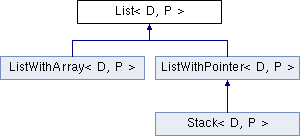
\includegraphics[height=3.000000cm]{class_list}
\end{center}
\end{figure}
\subsection*{Public Member Functions}
\begin{DoxyCompactItemize}
\item 
\hyperlink{class_list_a3deb54ab4f51c6c39aa4015f258b5812}{List} ()
\begin{DoxyCompactList}\small\item\em Constructor de la clase \hyperlink{class_list}{List}. \end{DoxyCompactList}\item 
virtual \hyperlink{class_list_a624593fb77847bf7ad4cacfba3442471}{$\sim$\+List} ()
\begin{DoxyCompactList}\small\item\em Destructor de la clase \hyperlink{class_list}{List}. \end{DoxyCompactList}\item 
virtual void \hyperlink{class_list_a01f588d87d47f8332928eca38f7b11bb}{insert} (D d)=0
\begin{DoxyCompactList}\small\item\em Metodo virtual puro para insercion de datos en \hyperlink{class_list}{List}. \end{DoxyCompactList}\item 
virtual void \hyperlink{class_list_a14fc4e853102018df78db3899aa00d71}{remove} (D d)=0
\begin{DoxyCompactList}\small\item\em Metodo virtual puro para la remocion de un dato especifico de \hyperlink{class_list}{List}. \end{DoxyCompactList}\item 
virtual P \hyperlink{class_list_a2b40d6fffc7b2fb5138b648f52c839ee}{find} (D d)=0
\begin{DoxyCompactList}\small\item\em Metodo virtual puro para la busqueda de un dato especifico en \hyperlink{class_list}{List}. \end{DoxyCompactList}\item 
virtual D \hyperlink{class_list_a5bd565e668247ae0691983227367cc88}{get} (P k)=0
\begin{DoxyCompactList}\small\item\em Metodo virtual puro para obtener un dato en \hyperlink{class_list}{List}. \end{DoxyCompactList}\item 
virtual void \hyperlink{class_list_acb062aa988f4048498b30a2d845a311b}{assign} (P k, D d)=0
\begin{DoxyCompactList}\small\item\em Metodo virtual puro para asignar un valor especifico a un dato en \hyperlink{class_list}{List}. \end{DoxyCompactList}\item 
virtual void \hyperlink{class_list_ae3795939f27cf3e688cd470450e0c27a}{sort} ()=0
\begin{DoxyCompactList}\small\item\em Metodo virtual puro para ordenar \hyperlink{class_list}{List}. \end{DoxyCompactList}\item 
virtual int \hyperlink{class_list_af213bbcf13ee436a0f04cde66e337672}{get\+Size} ()=0
\begin{DoxyCompactList}\small\item\em Metodo virtual puro para obtener el tamaño de \hyperlink{class_list}{List}. \end{DoxyCompactList}\item 
virtual void \hyperlink{class_list_a8b34931e187e7e6b86aad86510ce4f3b}{print\+List} ()=0
\begin{DoxyCompactList}\small\item\em Metodo virtual puro para imrprimir \hyperlink{class_list}{List}. \end{DoxyCompactList}\item 
virtual P \hyperlink{class_list_a4ec3e88e176bb45bc49b030d1c8abb3f}{next} (P k)=0
\begin{DoxyCompactList}\small\item\em Metodo virtual puro para obtener el siguiente elemento de una posicion especifica de \hyperlink{class_list}{List}. \end{DoxyCompactList}\item 
virtual P \hyperlink{class_list_acc1831ae92a288345ef20cb29f3846b2}{prev} (P k)=0
\begin{DoxyCompactList}\small\item\em Metodo virtual puro para obtener el elemento anterior de una posicion especifica de \hyperlink{class_list}{List}. \end{DoxyCompactList}\item 
virtual void \hyperlink{class_list_a24b4f177a70215980e81ef7b2981fa1e}{empty\+List} ()=0
\begin{DoxyCompactList}\small\item\em Metodo virtual puro para vaciar \hyperlink{class_list}{List}\+: Deja sin ningun elemento \hyperlink{class_list}{List}. \end{DoxyCompactList}\end{DoxyCompactItemize}
\subsection*{Protected Attributes}
\begin{DoxyCompactItemize}
\item 
int \hyperlink{class_list_aa61221b9bda8b2b56a61bd869daacbfd}{n}
\begin{DoxyCompactList}\small\item\em Atrib. \end{DoxyCompactList}\item 
P \hyperlink{class_list_a32b9741aa48daca064edf0e83abf7a0f}{last}
\begin{DoxyCompactList}\small\item\em Atrib. \end{DoxyCompactList}\end{DoxyCompactItemize}


\subsection{Detailed Description}
\subsubsection*{template$<$typename D, typename P$>$class List$<$ D, P $>$}

Libreria que genera un template de una clase abstracta list. 

\begin{DoxyAuthor}{Author}
Luis Adrian Aguilar -\/ B00092 

Robin Gonzalez Ricz -\/ B43011 

Giancarlo Marin -\/ B54099 
\end{DoxyAuthor}
\begin{DoxyDate}{Date}
21-\/02-\/2017 Libreria que genera un template de una clase abstracta list que toma un tipo de dato para los datos contenidos en la lista (D) y otro para los indices de las misma (P) 
\end{DoxyDate}


\subsection{Constructor \& Destructor Documentation}
\hypertarget{class_list_a3deb54ab4f51c6c39aa4015f258b5812}{\index{List@{List}!List@{List}}
\index{List@{List}!List@{List}}
\subsubsection[{List}]{\setlength{\rightskip}{0pt plus 5cm}template$<$typename D , typename P $>$ {\bf List}$<$ D, P $>$\+::{\bf List} (
\begin{DoxyParamCaption}
{}
\end{DoxyParamCaption}
)\hspace{0.3cm}{\ttfamily [inline]}}}\label{class_list_a3deb54ab4f51c6c39aa4015f258b5812}


Constructor de la clase \hyperlink{class_list}{List}. 

\hypertarget{class_list_a624593fb77847bf7ad4cacfba3442471}{\index{List@{List}!````~List@{$\sim$\+List}}
\index{````~List@{$\sim$\+List}!List@{List}}
\subsubsection[{$\sim$\+List}]{\setlength{\rightskip}{0pt plus 5cm}template$<$typename D , typename P $>$ virtual {\bf List}$<$ D, P $>$\+::$\sim${\bf List} (
\begin{DoxyParamCaption}
{}
\end{DoxyParamCaption}
)\hspace{0.3cm}{\ttfamily [inline]}, {\ttfamily [virtual]}}}\label{class_list_a624593fb77847bf7ad4cacfba3442471}


Destructor de la clase \hyperlink{class_list}{List}. 



\subsection{Member Function Documentation}
\hypertarget{class_list_acb062aa988f4048498b30a2d845a311b}{\index{List@{List}!assign@{assign}}
\index{assign@{assign}!List@{List}}
\subsubsection[{assign}]{\setlength{\rightskip}{0pt plus 5cm}template$<$typename D , typename P $>$ virtual void {\bf List}$<$ D, P $>$\+::assign (
\begin{DoxyParamCaption}
\item[{P}]{k, }
\item[{D}]{d}
\end{DoxyParamCaption}
)\hspace{0.3cm}{\ttfamily [pure virtual]}}}\label{class_list_acb062aa988f4048498b30a2d845a311b}


Metodo virtual puro para asignar un valor especifico a un dato en \hyperlink{class_list}{List}. 


\begin{DoxyParams}{Parameters}
{\em k} & Indice de tipo P dentro de list donde se asignara el nuevo valor \\
\hline
{\em d} & Dato de tipo D que se asigna en la posicion k \\
\hline
\end{DoxyParams}


Implemented in \hyperlink{class_list_with_array_a9dd1fd2337c6c8d437de71aae0e816c8}{List\+With\+Array$<$ D, P $>$}, and \hyperlink{class_list_with_pointer_aeaa834b22c4d7276a77ff29df3da7a30}{List\+With\+Pointer$<$ D, P $>$}.

\hypertarget{class_list_a24b4f177a70215980e81ef7b2981fa1e}{\index{List@{List}!empty\+List@{empty\+List}}
\index{empty\+List@{empty\+List}!List@{List}}
\subsubsection[{empty\+List}]{\setlength{\rightskip}{0pt plus 5cm}template$<$typename D , typename P $>$ virtual void {\bf List}$<$ D, P $>$\+::empty\+List (
\begin{DoxyParamCaption}
{}
\end{DoxyParamCaption}
)\hspace{0.3cm}{\ttfamily [pure virtual]}}}\label{class_list_a24b4f177a70215980e81ef7b2981fa1e}


Metodo virtual puro para vaciar \hyperlink{class_list}{List}\+: Deja sin ningun elemento \hyperlink{class_list}{List}. 



Implemented in \hyperlink{class_list_with_pointer_aec4f5374971962c79d397bbcd0080199}{List\+With\+Pointer$<$ D, P $>$}, and \hyperlink{class_list_with_array_a2179e228f285cc29b46bd5d13ba0b4ed}{List\+With\+Array$<$ D, P $>$}.

\hypertarget{class_list_a2b40d6fffc7b2fb5138b648f52c839ee}{\index{List@{List}!find@{find}}
\index{find@{find}!List@{List}}
\subsubsection[{find}]{\setlength{\rightskip}{0pt plus 5cm}template$<$typename D , typename P $>$ virtual P {\bf List}$<$ D, P $>$\+::find (
\begin{DoxyParamCaption}
\item[{D}]{d}
\end{DoxyParamCaption}
)\hspace{0.3cm}{\ttfamily [pure virtual]}}}\label{class_list_a2b40d6fffc7b2fb5138b648f52c839ee}


Metodo virtual puro para la busqueda de un dato especifico en \hyperlink{class_list}{List}. 


\begin{DoxyParams}{Parameters}
{\em d} & Dato que se desea buscar en \hyperlink{class_list}{List} \\
\hline
\end{DoxyParams}
\begin{DoxyReturn}{Returns}
Indice de tipo P dentro de \hyperlink{class_list}{List} 
\end{DoxyReturn}


Implemented in \hyperlink{class_stack_aa8a3a0b773900e44f641e3be9d9345da}{Stack$<$ D, P $>$}, \hyperlink{class_list_with_array_a9a054a6d407dc5cb39575739fe412fff}{List\+With\+Array$<$ D, P $>$}, \hyperlink{class_queue_a5c5ad7000d15506d3ec9c2ef6c8e6041}{Queue$<$ D, P $>$}, and \hyperlink{class_list_with_pointer_afeff8b963c197378553e2a3f73eaf66a}{List\+With\+Pointer$<$ D, P $>$}.

\hypertarget{class_list_a5bd565e668247ae0691983227367cc88}{\index{List@{List}!get@{get}}
\index{get@{get}!List@{List}}
\subsubsection[{get}]{\setlength{\rightskip}{0pt plus 5cm}template$<$typename D , typename P $>$ virtual D {\bf List}$<$ D, P $>$\+::get (
\begin{DoxyParamCaption}
\item[{P}]{k}
\end{DoxyParamCaption}
)\hspace{0.3cm}{\ttfamily [pure virtual]}}}\label{class_list_a5bd565e668247ae0691983227367cc88}


Metodo virtual puro para obtener un dato en \hyperlink{class_list}{List}. 


\begin{DoxyParams}{Parameters}
{\em k} & Indice de tipo P dentro de \hyperlink{class_list}{List} del que se desea obtener dato \\
\hline
\end{DoxyParams}
\begin{DoxyReturn}{Returns}
Dato contenido en k de tipo D 
\end{DoxyReturn}


Implemented in \hyperlink{class_list_with_array_a20cfc82811967bc2a77a6e43b9cebb46}{List\+With\+Array$<$ D, P $>$}, and \hyperlink{class_list_with_pointer_a0ff36c852334da8bc167356e636c1846}{List\+With\+Pointer$<$ D, P $>$}.

\hypertarget{class_list_af213bbcf13ee436a0f04cde66e337672}{\index{List@{List}!get\+Size@{get\+Size}}
\index{get\+Size@{get\+Size}!List@{List}}
\subsubsection[{get\+Size}]{\setlength{\rightskip}{0pt plus 5cm}template$<$typename D , typename P $>$ virtual int {\bf List}$<$ D, P $>$\+::get\+Size (
\begin{DoxyParamCaption}
{}
\end{DoxyParamCaption}
)\hspace{0.3cm}{\ttfamily [pure virtual]}}}\label{class_list_af213bbcf13ee436a0f04cde66e337672}


Metodo virtual puro para obtener el tamaño de \hyperlink{class_list}{List}. 



Implemented in \hyperlink{class_list_with_pointer_ac70c49b5703887fd867e90cdac3c706f}{List\+With\+Pointer$<$ D, P $>$}, \hyperlink{class_list_with_array_ae7a071bcdde9ddbf4c40a716f5a09434}{List\+With\+Array$<$ D, P $>$}, \hyperlink{class_stack_a74fc7e5921dfb247f9ad7052c3c4297a}{Stack$<$ D, P $>$}, and \hyperlink{class_queue_ab2c7217e6737bf579493b321184a2db3}{Queue$<$ D, P $>$}.

\hypertarget{class_list_a01f588d87d47f8332928eca38f7b11bb}{\index{List@{List}!insert@{insert}}
\index{insert@{insert}!List@{List}}
\subsubsection[{insert}]{\setlength{\rightskip}{0pt plus 5cm}template$<$typename D , typename P $>$ virtual void {\bf List}$<$ D, P $>$\+::insert (
\begin{DoxyParamCaption}
\item[{D}]{d}
\end{DoxyParamCaption}
)\hspace{0.3cm}{\ttfamily [pure virtual]}}}\label{class_list_a01f588d87d47f8332928eca38f7b11bb}


Metodo virtual puro para insercion de datos en \hyperlink{class_list}{List}. 


\begin{DoxyParams}{Parameters}
{\em d} & Dato de tipo D que se desea insertar en \hyperlink{class_list}{List} \\
\hline
\end{DoxyParams}


Implemented in \hyperlink{class_list_with_array_afa0b6d215c2cc1d3fe6b9b48d6b6917d}{List\+With\+Array$<$ D, P $>$}, and \hyperlink{class_list_with_pointer_a676e57683ade8e179e8eff5885f7309a}{List\+With\+Pointer$<$ D, P $>$}.

\hypertarget{class_list_a4ec3e88e176bb45bc49b030d1c8abb3f}{\index{List@{List}!next@{next}}
\index{next@{next}!List@{List}}
\subsubsection[{next}]{\setlength{\rightskip}{0pt plus 5cm}template$<$typename D , typename P $>$ virtual P {\bf List}$<$ D, P $>$\+::next (
\begin{DoxyParamCaption}
\item[{P}]{k}
\end{DoxyParamCaption}
)\hspace{0.3cm}{\ttfamily [pure virtual]}}}\label{class_list_a4ec3e88e176bb45bc49b030d1c8abb3f}


Metodo virtual puro para obtener el siguiente elemento de una posicion especifica de \hyperlink{class_list}{List}. 


\begin{DoxyParams}{Parameters}
{\em k} & Indice de tipo P dentro de \hyperlink{class_list}{List} del que se desea el siguiente elemento \\
\hline
\end{DoxyParams}
\begin{DoxyReturn}{Returns}
Siguiente elemento de k de tipo P 
\end{DoxyReturn}


Implemented in \hyperlink{class_list_with_pointer_a518b5ee89e3ad32ae7cd4ddd5d4fa7e9}{List\+With\+Pointer$<$ D, P $>$}, \hyperlink{class_list_with_array_a125811011abb77c1b11e5150f4524fb1}{List\+With\+Array$<$ D, P $>$}, \hyperlink{class_queue_aa4c9b83f260a172e1fffc389f354386f}{Queue$<$ D, P $>$}, and \hyperlink{class_stack_ab7f8f7e4ab10c00769c1debc5391fc17}{Stack$<$ D, P $>$}.

\hypertarget{class_list_acc1831ae92a288345ef20cb29f3846b2}{\index{List@{List}!prev@{prev}}
\index{prev@{prev}!List@{List}}
\subsubsection[{prev}]{\setlength{\rightskip}{0pt plus 5cm}template$<$typename D , typename P $>$ virtual P {\bf List}$<$ D, P $>$\+::prev (
\begin{DoxyParamCaption}
\item[{P}]{k}
\end{DoxyParamCaption}
)\hspace{0.3cm}{\ttfamily [pure virtual]}}}\label{class_list_acc1831ae92a288345ef20cb29f3846b2}


Metodo virtual puro para obtener el elemento anterior de una posicion especifica de \hyperlink{class_list}{List}. 


\begin{DoxyParams}{Parameters}
{\em k} & Indice de tipo P dentro de \hyperlink{class_list}{List} del que se desea el elemento anterior \\
\hline
\end{DoxyParams}
\begin{DoxyReturn}{Returns}
Elemento anterior de k de tipo P 
\end{DoxyReturn}


Implemented in \hyperlink{class_list_with_pointer_a7242068fcc3a193f0f7e94517856e431}{List\+With\+Pointer$<$ D, P $>$}, \hyperlink{class_list_with_array_a72f0d74c4ae1fd4697088114db41d442}{List\+With\+Array$<$ D, P $>$}, \hyperlink{class_queue_adcb9a0e709ea65bc7e98f7e9cbae8a39}{Queue$<$ D, P $>$}, and \hyperlink{class_stack_a0c0b55f72c9249bfb9252bce1a93458d}{Stack$<$ D, P $>$}.

\hypertarget{class_list_a8b34931e187e7e6b86aad86510ce4f3b}{\index{List@{List}!print\+List@{print\+List}}
\index{print\+List@{print\+List}!List@{List}}
\subsubsection[{print\+List}]{\setlength{\rightskip}{0pt plus 5cm}template$<$typename D , typename P $>$ virtual void {\bf List}$<$ D, P $>$\+::print\+List (
\begin{DoxyParamCaption}
{}
\end{DoxyParamCaption}
)\hspace{0.3cm}{\ttfamily [pure virtual]}}}\label{class_list_a8b34931e187e7e6b86aad86510ce4f3b}


Metodo virtual puro para imrprimir \hyperlink{class_list}{List}. 



Implemented in \hyperlink{class_list_with_pointer_a7079b5f1dbddb87a7e33ffc71ebb7b92}{List\+With\+Pointer$<$ D, P $>$}, and \hyperlink{class_list_with_array_a515ea38cb40ba7b0c9df98825b2dd270}{List\+With\+Array$<$ D, P $>$}.

\hypertarget{class_list_a14fc4e853102018df78db3899aa00d71}{\index{List@{List}!remove@{remove}}
\index{remove@{remove}!List@{List}}
\subsubsection[{remove}]{\setlength{\rightskip}{0pt plus 5cm}template$<$typename D , typename P $>$ virtual void {\bf List}$<$ D, P $>$\+::remove (
\begin{DoxyParamCaption}
\item[{D}]{d}
\end{DoxyParamCaption}
)\hspace{0.3cm}{\ttfamily [pure virtual]}}}\label{class_list_a14fc4e853102018df78db3899aa00d71}


Metodo virtual puro para la remocion de un dato especifico de \hyperlink{class_list}{List}. 


\begin{DoxyParams}{Parameters}
{\em d} & Dato de tipo D que se desea remover de \hyperlink{class_list}{List} \\
\hline
\end{DoxyParams}


Implemented in \hyperlink{class_list_with_array_aaa18e76fc128ca05151178d914901ec3}{List\+With\+Array$<$ D, P $>$}, and \hyperlink{class_list_with_pointer_abcb151e95e9fffea7f9f7af593d8176f}{List\+With\+Pointer$<$ D, P $>$}.

\hypertarget{class_list_ae3795939f27cf3e688cd470450e0c27a}{\index{List@{List}!sort@{sort}}
\index{sort@{sort}!List@{List}}
\subsubsection[{sort}]{\setlength{\rightskip}{0pt plus 5cm}template$<$typename D , typename P $>$ virtual void {\bf List}$<$ D, P $>$\+::sort (
\begin{DoxyParamCaption}
{}
\end{DoxyParamCaption}
)\hspace{0.3cm}{\ttfamily [pure virtual]}}}\label{class_list_ae3795939f27cf3e688cd470450e0c27a}


Metodo virtual puro para ordenar \hyperlink{class_list}{List}. 



Implemented in \hyperlink{class_list_with_array_a1a0ec4ab4a8fcb1a20568445ad892c9a}{List\+With\+Array$<$ D, P $>$}, \hyperlink{class_list_with_pointer_aa46631b2da29895d1f767626fb591bc8}{List\+With\+Pointer$<$ D, P $>$}, and \hyperlink{class_queue_a896b0e1bcac0d660079eb838c1823446}{Queue$<$ D, P $>$}.



\subsection{Member Data Documentation}
\hypertarget{class_list_a32b9741aa48daca064edf0e83abf7a0f}{\index{List@{List}!last@{last}}
\index{last@{last}!List@{List}}
\subsubsection[{last}]{\setlength{\rightskip}{0pt plus 5cm}template$<$typename D , typename P $>$ P {\bf List}$<$ D, P $>$\+::last\hspace{0.3cm}{\ttfamily [protected]}}}\label{class_list_a32b9741aa48daca064edf0e83abf7a0f}


Atrib. 

protegido de tipo P que indica el indice del ultimo elemento de list \hypertarget{class_list_aa61221b9bda8b2b56a61bd869daacbfd}{\index{List@{List}!n@{n}}
\index{n@{n}!List@{List}}
\subsubsection[{n}]{\setlength{\rightskip}{0pt plus 5cm}template$<$typename D , typename P $>$ int {\bf List}$<$ D, P $>$\+::n\hspace{0.3cm}{\ttfamily [protected]}}}\label{class_list_aa61221b9bda8b2b56a61bd869daacbfd}


Atrib. 

protegido de tipo entero que indica el numero de elementos en list 

The documentation for this class was generated from the following file\+:\begin{DoxyCompactItemize}
\item 
include/\hyperlink{_list_8h}{List.\+h}\end{DoxyCompactItemize}

\hypertarget{class_list_with_array}{\section{List\+With\+Array$<$ D, P $>$ Class Template Reference}
\label{class_list_with_array}\index{List\+With\+Array$<$ D, P $>$@{List\+With\+Array$<$ D, P $>$}}
}


Libreria que genera un template de una clase \hyperlink{class_list_with_array}{List\+With\+Array} (lista implementada con arreglos) que hereda de la clase \hyperlink{class_list}{List} y que toma un tipo de dato para los datos contenidos en la lista (D) y otro para los indices de las misma (P)  




{\ttfamily \#include $<$List\+With\+Array.\+h$>$}



Inheritance diagram for List\+With\+Array$<$ D, P $>$\+:


Collaboration diagram for List\+With\+Array$<$ D, P $>$\+:
\subsection*{Public Member Functions}
\begin{DoxyCompactItemize}
\item 
\hyperlink{class_list_with_array_a06f0e8035e9cc43aff4d32c46a00fcf0}{List\+With\+Array} ()
\begin{DoxyCompactList}\small\item\em Constructor de la clase \hyperlink{class_list_with_array}{List\+With\+Array}. \end{DoxyCompactList}\item 
\hyperlink{class_list_with_array_a3a6d11f203fb0f7e458672e85db26b03}{List\+With\+Array} (int t)
\begin{DoxyCompactList}\small\item\em Constructor sobrecargado de la clase \hyperlink{class_list_with_array}{List\+With\+Array}. \end{DoxyCompactList}\item 
\hyperlink{class_list_with_array_a1886482555430b0f3eb5ebe02cbb0c87}{$\sim$\+List\+With\+Array} ()
\begin{DoxyCompactList}\small\item\em Destructor de la clase \hyperlink{class_list_with_array}{List\+With\+Array}. \end{DoxyCompactList}\item 
void \hyperlink{class_list_with_array_afa0b6d215c2cc1d3fe6b9b48d6b6917d}{insert} (\hyperlink{main_8cpp_af316c33cc298530f245e8b55330e86b5}{D} d)
\begin{DoxyCompactList}\small\item\em Metodo que implementa la insercion para \hyperlink{class_list_with_array}{List\+With\+Array}. \end{DoxyCompactList}\item 
void \hyperlink{class_list_with_array_aaa18e76fc128ca05151178d914901ec3}{remove} (\hyperlink{main_8cpp_af316c33cc298530f245e8b55330e86b5}{D} d)
\begin{DoxyCompactList}\small\item\em Metodo que implementa la remocion para \hyperlink{class_list_with_array}{List\+With\+Array}. \end{DoxyCompactList}\item 
P \hyperlink{class_list_with_array_a9a054a6d407dc5cb39575739fe412fff}{find} (\hyperlink{main_8cpp_af316c33cc298530f245e8b55330e86b5}{D} d)
\begin{DoxyCompactList}\small\item\em Metodo que implementa la busqueda para \hyperlink{class_list_with_array}{List\+With\+Array}. \end{DoxyCompactList}\item 
\hyperlink{main_8cpp_af316c33cc298530f245e8b55330e86b5}{D} \hyperlink{class_list_with_array_a20cfc82811967bc2a77a6e43b9cebb46}{get} (P k)
\begin{DoxyCompactList}\small\item\em Metodo que implementa el obtener un dato para \hyperlink{class_list_with_array}{List\+With\+Array}. \end{DoxyCompactList}\item 
void \hyperlink{class_list_with_array_a9dd1fd2337c6c8d437de71aae0e816c8}{assign} (P k, \hyperlink{main_8cpp_af316c33cc298530f245e8b55330e86b5}{D} d)
\begin{DoxyCompactList}\small\item\em Metodo que implementa el asignar un valor especifico a un dato en \hyperlink{class_list_with_array}{List\+With\+Array}. \end{DoxyCompactList}\item 
void \hyperlink{class_list_with_array_a1a0ec4ab4a8fcb1a20568445ad892c9a}{sort} ()
\begin{DoxyCompactList}\small\item\em Metodo que implementa el ordenar para \hyperlink{class_list_with_array}{List\+With\+Array}. \end{DoxyCompactList}\item 
int \hyperlink{class_list_with_array_ae7a071bcdde9ddbf4c40a716f5a09434}{get\+Size} ()
\begin{DoxyCompactList}\small\item\em Metodo que implementa el obtener tamaño de \hyperlink{class_list_with_array}{List\+With\+Array}. \end{DoxyCompactList}\item 
void \hyperlink{class_list_with_array_a515ea38cb40ba7b0c9df98825b2dd270}{print\+List} ()
\begin{DoxyCompactList}\small\item\em Metodo que implementa el imrprimir lista para \hyperlink{class_list_with_array}{List\+With\+Array}. \end{DoxyCompactList}\item 
P \hyperlink{class_list_with_array_a125811011abb77c1b11e5150f4524fb1}{next} (P k)
\begin{DoxyCompactList}\small\item\em Metodo que implementa el obtener siguiente elemento de una posicion especifica de \hyperlink{class_list_with_array}{List\+With\+Array}. \end{DoxyCompactList}\item 
P \hyperlink{class_list_with_array_a72f0d74c4ae1fd4697088114db41d442}{prev} (P k)
\begin{DoxyCompactList}\small\item\em Metodo que implementa el obtener elemento anterior de una posicion especifica de \hyperlink{class_list_with_array}{List\+With\+Array}. \end{DoxyCompactList}\item 
void \hyperlink{class_list_with_array_a2179e228f285cc29b46bd5d13ba0b4ed}{empty\+List} ()
\begin{DoxyCompactList}\small\item\em Metodo que implementa el vaciar Lista que Deja sin ningun elemento a \hyperlink{class_list_with_array}{List\+With\+Array}. \end{DoxyCompactList}\end{DoxyCompactItemize}
\subsection*{Additional Inherited Members}


\subsection{Detailed Description}
\subsubsection*{template$<$typename D, typename P$>$class List\+With\+Array$<$ D, P $>$}

Libreria que genera un template de una clase \hyperlink{class_list_with_array}{List\+With\+Array} (lista implementada con arreglos) que hereda de la clase \hyperlink{class_list}{List} y que toma un tipo de dato para los datos contenidos en la lista (D) y otro para los indices de las misma (P) 

Definition at line 16 of file List\+With\+Array.\+h.



\subsection{Constructor \& Destructor Documentation}
\hypertarget{class_list_with_array_a06f0e8035e9cc43aff4d32c46a00fcf0}{\index{List\+With\+Array@{List\+With\+Array}!List\+With\+Array@{List\+With\+Array}}
\index{List\+With\+Array@{List\+With\+Array}!List\+With\+Array@{List\+With\+Array}}
\subsubsection[{List\+With\+Array}]{\setlength{\rightskip}{0pt plus 5cm}template$<$typename D, typename P$>$ {\bf List\+With\+Array}$<$ {\bf D}, P $>$\+::{\bf List\+With\+Array} (
\begin{DoxyParamCaption}
{}
\end{DoxyParamCaption}
)\hspace{0.3cm}{\ttfamily [inline]}}}\label{class_list_with_array_a06f0e8035e9cc43aff4d32c46a00fcf0}


Constructor de la clase \hyperlink{class_list_with_array}{List\+With\+Array}. 



Definition at line 22 of file List\+With\+Array.\+h.

\hypertarget{class_list_with_array_a3a6d11f203fb0f7e458672e85db26b03}{\index{List\+With\+Array@{List\+With\+Array}!List\+With\+Array@{List\+With\+Array}}
\index{List\+With\+Array@{List\+With\+Array}!List\+With\+Array@{List\+With\+Array}}
\subsubsection[{List\+With\+Array}]{\setlength{\rightskip}{0pt plus 5cm}template$<$typename D, typename P$>$ {\bf List\+With\+Array}$<$ {\bf D}, P $>$\+::{\bf List\+With\+Array} (
\begin{DoxyParamCaption}
\item[{int}]{t}
\end{DoxyParamCaption}
)\hspace{0.3cm}{\ttfamily [inline]}}}\label{class_list_with_array_a3a6d11f203fb0f7e458672e85db26b03}


Constructor sobrecargado de la clase \hyperlink{class_list_with_array}{List\+With\+Array}. 


\begin{DoxyParams}{Parameters}
{\em t} & Entero que determina la cantidad maxima de elementon que puede contener la lista \\
\hline
\end{DoxyParams}


Definition at line 32 of file List\+With\+Array.\+h.

\hypertarget{class_list_with_array_a1886482555430b0f3eb5ebe02cbb0c87}{\index{List\+With\+Array@{List\+With\+Array}!````~List\+With\+Array@{$\sim$\+List\+With\+Array}}
\index{````~List\+With\+Array@{$\sim$\+List\+With\+Array}!List\+With\+Array@{List\+With\+Array}}
\subsubsection[{$\sim$\+List\+With\+Array}]{\setlength{\rightskip}{0pt plus 5cm}template$<$typename D, typename P$>$ {\bf List\+With\+Array}$<$ {\bf D}, P $>$\+::$\sim${\bf List\+With\+Array} (
\begin{DoxyParamCaption}
{}
\end{DoxyParamCaption}
)\hspace{0.3cm}{\ttfamily [inline]}}}\label{class_list_with_array_a1886482555430b0f3eb5ebe02cbb0c87}


Destructor de la clase \hyperlink{class_list_with_array}{List\+With\+Array}. 



Definition at line 41 of file List\+With\+Array.\+h.



\subsection{Member Function Documentation}
\hypertarget{class_list_with_array_a9dd1fd2337c6c8d437de71aae0e816c8}{\index{List\+With\+Array@{List\+With\+Array}!assign@{assign}}
\index{assign@{assign}!List\+With\+Array@{List\+With\+Array}}
\subsubsection[{assign}]{\setlength{\rightskip}{0pt plus 5cm}template$<$typename D, typename P$>$ void {\bf List\+With\+Array}$<$ {\bf D}, P $>$\+::assign (
\begin{DoxyParamCaption}
\item[{P}]{k, }
\item[{{\bf D}}]{d}
\end{DoxyParamCaption}
)\hspace{0.3cm}{\ttfamily [inline]}, {\ttfamily [virtual]}}}\label{class_list_with_array_a9dd1fd2337c6c8d437de71aae0e816c8}


Metodo que implementa el asignar un valor especifico a un dato en \hyperlink{class_list_with_array}{List\+With\+Array}. 


\begin{DoxyParams}{Parameters}
{\em k} & Indice de tipo P dentro de list donde se asignara el nuevo valor \\
\hline
{\em d} & Dato de tipo D que se asigna en la posicion k \\
\hline
\end{DoxyParams}


Implements \hyperlink{class_list_acb062aa988f4048498b30a2d845a311b}{List$<$ D, P $>$}.



Definition at line 122 of file List\+With\+Array.\+h.

\hypertarget{class_list_with_array_a2179e228f285cc29b46bd5d13ba0b4ed}{\index{List\+With\+Array@{List\+With\+Array}!empty\+List@{empty\+List}}
\index{empty\+List@{empty\+List}!List\+With\+Array@{List\+With\+Array}}
\subsubsection[{empty\+List}]{\setlength{\rightskip}{0pt plus 5cm}template$<$typename D, typename P$>$ void {\bf List\+With\+Array}$<$ {\bf D}, P $>$\+::empty\+List (
\begin{DoxyParamCaption}
{}
\end{DoxyParamCaption}
)\hspace{0.3cm}{\ttfamily [inline]}, {\ttfamily [virtual]}}}\label{class_list_with_array_a2179e228f285cc29b46bd5d13ba0b4ed}


Metodo que implementa el vaciar Lista que Deja sin ningun elemento a \hyperlink{class_list_with_array}{List\+With\+Array}. 



Implements \hyperlink{class_list_a24b4f177a70215980e81ef7b2981fa1e}{List$<$ D, P $>$}.



Definition at line 190 of file List\+With\+Array.\+h.

\hypertarget{class_list_with_array_a9a054a6d407dc5cb39575739fe412fff}{\index{List\+With\+Array@{List\+With\+Array}!find@{find}}
\index{find@{find}!List\+With\+Array@{List\+With\+Array}}
\subsubsection[{find}]{\setlength{\rightskip}{0pt plus 5cm}template$<$typename D, typename P$>$ P {\bf List\+With\+Array}$<$ {\bf D}, P $>$\+::find (
\begin{DoxyParamCaption}
\item[{{\bf D}}]{d}
\end{DoxyParamCaption}
)\hspace{0.3cm}{\ttfamily [inline]}, {\ttfamily [virtual]}}}\label{class_list_with_array_a9a054a6d407dc5cb39575739fe412fff}


Metodo que implementa la busqueda para \hyperlink{class_list_with_array}{List\+With\+Array}. 


\begin{DoxyParams}{Parameters}
{\em d} & Dato que se desea buscar en \hyperlink{class_list}{List} \\
\hline
\end{DoxyParams}
\begin{DoxyReturn}{Returns}
Indice de tipo P dentro de \hyperlink{class_list}{List} 
\end{DoxyReturn}
Indicacion de que el dato no fue encontrado en la lista 

Implements \hyperlink{class_list_a2b40d6fffc7b2fb5138b648f52c839ee}{List$<$ D, P $>$}.



Definition at line 100 of file List\+With\+Array.\+h.

\hypertarget{class_list_with_array_a20cfc82811967bc2a77a6e43b9cebb46}{\index{List\+With\+Array@{List\+With\+Array}!get@{get}}
\index{get@{get}!List\+With\+Array@{List\+With\+Array}}
\subsubsection[{get}]{\setlength{\rightskip}{0pt plus 5cm}template$<$typename D, typename P$>$ {\bf D} {\bf List\+With\+Array}$<$ {\bf D}, P $>$\+::get (
\begin{DoxyParamCaption}
\item[{P}]{k}
\end{DoxyParamCaption}
)\hspace{0.3cm}{\ttfamily [inline]}, {\ttfamily [virtual]}}}\label{class_list_with_array_a20cfc82811967bc2a77a6e43b9cebb46}


Metodo que implementa el obtener un dato para \hyperlink{class_list_with_array}{List\+With\+Array}. 


\begin{DoxyParams}{Parameters}
{\em k} & Indice de tipo P dentro de \hyperlink{class_list}{List} del que se desea obtener dato \\
\hline
\end{DoxyParams}
\begin{DoxyReturn}{Returns}
Dato contenido en k de tipo D 
\end{DoxyReturn}


Implements \hyperlink{class_list_a5bd565e668247ae0691983227367cc88}{List$<$ D, P $>$}.



Definition at line 113 of file List\+With\+Array.\+h.

\hypertarget{class_list_with_array_ae7a071bcdde9ddbf4c40a716f5a09434}{\index{List\+With\+Array@{List\+With\+Array}!get\+Size@{get\+Size}}
\index{get\+Size@{get\+Size}!List\+With\+Array@{List\+With\+Array}}
\subsubsection[{get\+Size}]{\setlength{\rightskip}{0pt plus 5cm}template$<$typename D, typename P$>$ int {\bf List\+With\+Array}$<$ {\bf D}, P $>$\+::get\+Size (
\begin{DoxyParamCaption}
{}
\end{DoxyParamCaption}
)\hspace{0.3cm}{\ttfamily [inline]}, {\ttfamily [virtual]}}}\label{class_list_with_array_ae7a071bcdde9ddbf4c40a716f5a09434}


Metodo que implementa el obtener tamaño de \hyperlink{class_list_with_array}{List\+With\+Array}. 



Implements \hyperlink{class_list_af213bbcf13ee436a0f04cde66e337672}{List$<$ D, P $>$}.



Definition at line 149 of file List\+With\+Array.\+h.

\hypertarget{class_list_with_array_afa0b6d215c2cc1d3fe6b9b48d6b6917d}{\index{List\+With\+Array@{List\+With\+Array}!insert@{insert}}
\index{insert@{insert}!List\+With\+Array@{List\+With\+Array}}
\subsubsection[{insert}]{\setlength{\rightskip}{0pt plus 5cm}template$<$typename D, typename P$>$ void {\bf List\+With\+Array}$<$ {\bf D}, P $>$\+::insert (
\begin{DoxyParamCaption}
\item[{{\bf D}}]{d}
\end{DoxyParamCaption}
)\hspace{0.3cm}{\ttfamily [inline]}, {\ttfamily [virtual]}}}\label{class_list_with_array_afa0b6d215c2cc1d3fe6b9b48d6b6917d}


Metodo que implementa la insercion para \hyperlink{class_list_with_array}{List\+With\+Array}. 


\begin{DoxyParams}{Parameters}
{\em d} & Dato de tipo D que se desea insertar en \hyperlink{class_list}{List} \\
\hline
\end{DoxyParams}


Implements \hyperlink{class_list_a01f588d87d47f8332928eca38f7b11bb}{List$<$ D, P $>$}.



Definition at line 50 of file List\+With\+Array.\+h.

\hypertarget{class_list_with_array_a125811011abb77c1b11e5150f4524fb1}{\index{List\+With\+Array@{List\+With\+Array}!next@{next}}
\index{next@{next}!List\+With\+Array@{List\+With\+Array}}
\subsubsection[{next}]{\setlength{\rightskip}{0pt plus 5cm}template$<$typename D, typename P$>$ P {\bf List\+With\+Array}$<$ {\bf D}, P $>$\+::next (
\begin{DoxyParamCaption}
\item[{P}]{k}
\end{DoxyParamCaption}
)\hspace{0.3cm}{\ttfamily [inline]}, {\ttfamily [virtual]}}}\label{class_list_with_array_a125811011abb77c1b11e5150f4524fb1}


Metodo que implementa el obtener siguiente elemento de una posicion especifica de \hyperlink{class_list_with_array}{List\+With\+Array}. 


\begin{DoxyParams}{Parameters}
{\em k} & Indice de tipo P dentro de \hyperlink{class_list}{List} del que se desea el siguiente elemento \\
\hline
\end{DoxyParams}
\begin{DoxyReturn}{Returns}
Siguiente elemento de k de tipo P 
\end{DoxyReturn}
Indicacion de que no hay dato siguiente en la lista 

Implements \hyperlink{class_list_a4ec3e88e176bb45bc49b030d1c8abb3f}{List$<$ D, P $>$}.



Definition at line 168 of file List\+With\+Array.\+h.

\hypertarget{class_list_with_array_a72f0d74c4ae1fd4697088114db41d442}{\index{List\+With\+Array@{List\+With\+Array}!prev@{prev}}
\index{prev@{prev}!List\+With\+Array@{List\+With\+Array}}
\subsubsection[{prev}]{\setlength{\rightskip}{0pt plus 5cm}template$<$typename D, typename P$>$ P {\bf List\+With\+Array}$<$ {\bf D}, P $>$\+::prev (
\begin{DoxyParamCaption}
\item[{P}]{k}
\end{DoxyParamCaption}
)\hspace{0.3cm}{\ttfamily [inline]}, {\ttfamily [virtual]}}}\label{class_list_with_array_a72f0d74c4ae1fd4697088114db41d442}


Metodo que implementa el obtener elemento anterior de una posicion especifica de \hyperlink{class_list_with_array}{List\+With\+Array}. 


\begin{DoxyParams}{Parameters}
{\em k} & Indice de tipo P dentro de \hyperlink{class_list}{List} del que se desea el elemento anterior \\
\hline
\end{DoxyParams}
\begin{DoxyReturn}{Returns}
Elemento anterior de k de tipo P 
\end{DoxyReturn}
Indicacion de que no hay dato anterior en la lista 

Implements \hyperlink{class_list_acc1831ae92a288345ef20cb29f3846b2}{List$<$ D, P $>$}.



Definition at line 180 of file List\+With\+Array.\+h.

\hypertarget{class_list_with_array_a515ea38cb40ba7b0c9df98825b2dd270}{\index{List\+With\+Array@{List\+With\+Array}!print\+List@{print\+List}}
\index{print\+List@{print\+List}!List\+With\+Array@{List\+With\+Array}}
\subsubsection[{print\+List}]{\setlength{\rightskip}{0pt plus 5cm}template$<$typename D, typename P$>$ void {\bf List\+With\+Array}$<$ {\bf D}, P $>$\+::print\+List (
\begin{DoxyParamCaption}
{}
\end{DoxyParamCaption}
)\hspace{0.3cm}{\ttfamily [inline]}, {\ttfamily [virtual]}}}\label{class_list_with_array_a515ea38cb40ba7b0c9df98825b2dd270}


Metodo que implementa el imrprimir lista para \hyperlink{class_list_with_array}{List\+With\+Array}. 



Implements \hyperlink{class_list_a8b34931e187e7e6b86aad86510ce4f3b}{List$<$ D, P $>$}.



Definition at line 156 of file List\+With\+Array.\+h.

\hypertarget{class_list_with_array_aaa18e76fc128ca05151178d914901ec3}{\index{List\+With\+Array@{List\+With\+Array}!remove@{remove}}
\index{remove@{remove}!List\+With\+Array@{List\+With\+Array}}
\subsubsection[{remove}]{\setlength{\rightskip}{0pt plus 5cm}template$<$typename D, typename P$>$ void {\bf List\+With\+Array}$<$ {\bf D}, P $>$\+::remove (
\begin{DoxyParamCaption}
\item[{{\bf D}}]{d}
\end{DoxyParamCaption}
)\hspace{0.3cm}{\ttfamily [inline]}, {\ttfamily [virtual]}}}\label{class_list_with_array_aaa18e76fc128ca05151178d914901ec3}


Metodo que implementa la remocion para \hyperlink{class_list_with_array}{List\+With\+Array}. 


\begin{DoxyParams}{Parameters}
{\em d} & Dato de tipo D que se desea remover de \hyperlink{class_list}{List} \\
\hline
\end{DoxyParams}
$<$entero que indica la posicion donde se debe remover 

Implements \hyperlink{class_list_a14fc4e853102018df78db3899aa00d71}{List$<$ D, P $>$}.



Definition at line 84 of file List\+With\+Array.\+h.

\hypertarget{class_list_with_array_a1a0ec4ab4a8fcb1a20568445ad892c9a}{\index{List\+With\+Array@{List\+With\+Array}!sort@{sort}}
\index{sort@{sort}!List\+With\+Array@{List\+With\+Array}}
\subsubsection[{sort}]{\setlength{\rightskip}{0pt plus 5cm}template$<$typename D, typename P$>$ void {\bf List\+With\+Array}$<$ {\bf D}, P $>$\+::sort (
\begin{DoxyParamCaption}
{}
\end{DoxyParamCaption}
)\hspace{0.3cm}{\ttfamily [inline]}, {\ttfamily [virtual]}}}\label{class_list_with_array_a1a0ec4ab4a8fcb1a20568445ad892c9a}


Metodo que implementa el ordenar para \hyperlink{class_list_with_array}{List\+With\+Array}. 

Implementacion por medio de Selection Sort 

Implements \hyperlink{class_list_ae3795939f27cf3e688cd470450e0c27a}{List$<$ D, P $>$}.



Definition at line 129 of file List\+With\+Array.\+h.



The documentation for this class was generated from the following file\+:\begin{DoxyCompactItemize}
\item 
include/\hyperlink{_list_with_array_8h}{List\+With\+Array.\+h}\end{DoxyCompactItemize}

\hypertarget{class_list_with_pointer}{\section{List\+With\+Pointer$<$ D, P $>$ Class Template Reference}
\label{class_list_with_pointer}\index{List\+With\+Pointer$<$ D, P $>$@{List\+With\+Pointer$<$ D, P $>$}}
}


Libreria que genera un template de una clase \hyperlink{class_list_with_pointer}{List\+With\+Pointer} (lista implementada con punteros) que hereda de la clase \hyperlink{class_list}{List} y que toma un tipo de dato para los datos contenidos en la lista (D) y otro para los indices de las misma (P)  




{\ttfamily \#include $<$List\+With\+Pointer.\+h$>$}



Inheritance diagram for List\+With\+Pointer$<$ D, P $>$\+:


Collaboration diagram for List\+With\+Pointer$<$ D, P $>$\+:
\subsection*{Public Member Functions}
\begin{DoxyCompactItemize}
\item 
\hyperlink{class_list_with_pointer_a53b1284b13bf834bc5fc1eb27368a283}{List\+With\+Pointer} ()
\begin{DoxyCompactList}\small\item\em Constructor de la clase \hyperlink{class_list_with_pointer}{List\+With\+Pointer}. \end{DoxyCompactList}\item 
\hyperlink{class_list_with_pointer_a2a19c2e6e9bdee1c56750e36d6bbd7c2}{$\sim$\+List\+With\+Pointer} ()
\begin{DoxyCompactList}\small\item\em Destructor de la clase \hyperlink{class_list_with_pointer}{List\+With\+Pointer}. \end{DoxyCompactList}\item 
void \hyperlink{class_list_with_pointer_a676e57683ade8e179e8eff5885f7309a}{insert} (\hyperlink{gwp_2main_8cpp_af316c33cc298530f245e8b55330e86b5}{D} d)
\begin{DoxyCompactList}\small\item\em Metodo que implementa la insercion para \hyperlink{class_list_with_pointer}{List\+With\+Pointer}. \end{DoxyCompactList}\item 
void \hyperlink{class_list_with_pointer_abcb151e95e9fffea7f9f7af593d8176f}{remove} (\hyperlink{gwp_2main_8cpp_af316c33cc298530f245e8b55330e86b5}{D} d)
\begin{DoxyCompactList}\small\item\em Metodo que implementa la remocion para \hyperlink{class_list_with_pointer}{List\+With\+Pointer}. \end{DoxyCompactList}\item 
P \hyperlink{class_list_with_pointer_afeff8b963c197378553e2a3f73eaf66a}{find} (\hyperlink{gwp_2main_8cpp_af316c33cc298530f245e8b55330e86b5}{D} d)
\begin{DoxyCompactList}\small\item\em Metodo que implementa la busqueda para \hyperlink{class_list_with_pointer}{List\+With\+Pointer}. \end{DoxyCompactList}\item 
\hyperlink{gwp_2main_8cpp_af316c33cc298530f245e8b55330e86b5}{D} \hyperlink{class_list_with_pointer_a0ff36c852334da8bc167356e636c1846}{get} (P k)
\begin{DoxyCompactList}\small\item\em Metodo que implementa el obtener un dato para \hyperlink{class_list_with_pointer}{List\+With\+Pointer}. \end{DoxyCompactList}\item 
void \hyperlink{class_list_with_pointer_aeaa834b22c4d7276a77ff29df3da7a30}{assign} (P k, \hyperlink{gwp_2main_8cpp_af316c33cc298530f245e8b55330e86b5}{D} d)
\begin{DoxyCompactList}\small\item\em Metodo que implementa el asignar un valor especifico a un dato en \hyperlink{class_list_with_pointer}{List\+With\+Pointer}. \end{DoxyCompactList}\item 
int \hyperlink{class_list_with_pointer_ac70c49b5703887fd867e90cdac3c706f}{get\+Size} ()
\begin{DoxyCompactList}\small\item\em Metodo que implementa el ordenar para \hyperlink{class_list_with_pointer}{List\+With\+Pointer}. \end{DoxyCompactList}\item 
void \hyperlink{class_list_with_pointer_a7079b5f1dbddb87a7e33ffc71ebb7b92}{print\+List} ()
\begin{DoxyCompactList}\small\item\em Metodo que implementa el imrprimir lista para \hyperlink{class_list_with_pointer}{List\+With\+Pointer}. \end{DoxyCompactList}\item 
P \hyperlink{class_list_with_pointer_a518b5ee89e3ad32ae7cd4ddd5d4fa7e9}{next} (P k)
\begin{DoxyCompactList}\small\item\em Metodo que implementa el obtener siguiente elemento de una posicion especifica de \hyperlink{class_list_with_pointer}{List\+With\+Pointer}. \end{DoxyCompactList}\item 
P \hyperlink{class_list_with_pointer_a7242068fcc3a193f0f7e94517856e431}{prev} (P k)
\begin{DoxyCompactList}\small\item\em Metodo que implementa el obtener elemento anterior de una posicion especifica de \hyperlink{class_list_with_pointer}{List\+With\+Pointer}. \end{DoxyCompactList}\item 
void \hyperlink{class_list_with_pointer_aec4f5374971962c79d397bbcd0080199}{empty\+List} ()
\begin{DoxyCompactList}\small\item\em Metodo que implementa el vaciar Lista que Deja sin ningun elemento a \hyperlink{class_list_with_pointer}{List\+With\+Pointer}. \end{DoxyCompactList}\end{DoxyCompactItemize}
\subsection*{Public Attributes}
\begin{DoxyCompactItemize}
\item 
P \hyperlink{class_list_with_pointer_a10f9bcf73fcff6ca7fae28bec209bd20}{first}
\begin{DoxyCompactList}\small\item\em Atrib. \end{DoxyCompactList}\item 
P \hyperlink{class_list_with_pointer_aa4ff3f43dffeb524dc1cf3ac5dfdb415}{last}
\begin{DoxyCompactList}\small\item\em Atrib. \end{DoxyCompactList}\end{DoxyCompactItemize}
\subsection*{Additional Inherited Members}


\subsection{Detailed Description}
\subsubsection*{template$<$typename D, typename P$>$class List\+With\+Pointer$<$ D, P $>$}

Libreria que genera un template de una clase \hyperlink{class_list_with_pointer}{List\+With\+Pointer} (lista implementada con punteros) que hereda de la clase \hyperlink{class_list}{List} y que toma un tipo de dato para los datos contenidos en la lista (D) y otro para los indices de las misma (P) 

Definition at line 20 of file List\+With\+Pointer.\+h.



\subsection{Constructor \& Destructor Documentation}
\hypertarget{class_list_with_pointer_a53b1284b13bf834bc5fc1eb27368a283}{\index{List\+With\+Pointer@{List\+With\+Pointer}!List\+With\+Pointer@{List\+With\+Pointer}}
\index{List\+With\+Pointer@{List\+With\+Pointer}!List\+With\+Pointer@{List\+With\+Pointer}}
\subsubsection[{List\+With\+Pointer}]{\setlength{\rightskip}{0pt plus 5cm}template$<$typename D, typename P$>$ {\bf List\+With\+Pointer}$<$ {\bf D}, P $>$\+::{\bf List\+With\+Pointer} (
\begin{DoxyParamCaption}
{}
\end{DoxyParamCaption}
)\hspace{0.3cm}{\ttfamily [inline]}}}\label{class_list_with_pointer_a53b1284b13bf834bc5fc1eb27368a283}


Constructor de la clase \hyperlink{class_list_with_pointer}{List\+With\+Pointer}. 



Definition at line 26 of file List\+With\+Pointer.\+h.

\hypertarget{class_list_with_pointer_a2a19c2e6e9bdee1c56750e36d6bbd7c2}{\index{List\+With\+Pointer@{List\+With\+Pointer}!````~List\+With\+Pointer@{$\sim$\+List\+With\+Pointer}}
\index{````~List\+With\+Pointer@{$\sim$\+List\+With\+Pointer}!List\+With\+Pointer@{List\+With\+Pointer}}
\subsubsection[{$\sim$\+List\+With\+Pointer}]{\setlength{\rightskip}{0pt plus 5cm}template$<$typename D, typename P$>$ {\bf List\+With\+Pointer}$<$ {\bf D}, P $>$\+::$\sim${\bf List\+With\+Pointer} (
\begin{DoxyParamCaption}
{}
\end{DoxyParamCaption}
)\hspace{0.3cm}{\ttfamily [inline]}}}\label{class_list_with_pointer_a2a19c2e6e9bdee1c56750e36d6bbd7c2}


Destructor de la clase \hyperlink{class_list_with_pointer}{List\+With\+Pointer}. 



Definition at line 35 of file List\+With\+Pointer.\+h.



\subsection{Member Function Documentation}
\hypertarget{class_list_with_pointer_aeaa834b22c4d7276a77ff29df3da7a30}{\index{List\+With\+Pointer@{List\+With\+Pointer}!assign@{assign}}
\index{assign@{assign}!List\+With\+Pointer@{List\+With\+Pointer}}
\subsubsection[{assign}]{\setlength{\rightskip}{0pt plus 5cm}template$<$typename D, typename P$>$ void {\bf List\+With\+Pointer}$<$ {\bf D}, P $>$\+::assign (
\begin{DoxyParamCaption}
\item[{P}]{k, }
\item[{{\bf D}}]{d}
\end{DoxyParamCaption}
)\hspace{0.3cm}{\ttfamily [inline]}, {\ttfamily [virtual]}}}\label{class_list_with_pointer_aeaa834b22c4d7276a77ff29df3da7a30}


Metodo que implementa el asignar un valor especifico a un dato en \hyperlink{class_list_with_pointer}{List\+With\+Pointer}. 


\begin{DoxyParams}{Parameters}
{\em k} & Indice de tipo P dentro de list donde se asignara el nuevo valor \\
\hline
{\em d} & Dato de tipo D que se asigna en la posicion k \\
\hline
\end{DoxyParams}


Implements \hyperlink{class_list_acb062aa988f4048498b30a2d845a311b}{List$<$ D, P $>$}.



Definition at line 127 of file List\+With\+Pointer.\+h.

\hypertarget{class_list_with_pointer_aec4f5374971962c79d397bbcd0080199}{\index{List\+With\+Pointer@{List\+With\+Pointer}!empty\+List@{empty\+List}}
\index{empty\+List@{empty\+List}!List\+With\+Pointer@{List\+With\+Pointer}}
\subsubsection[{empty\+List}]{\setlength{\rightskip}{0pt plus 5cm}template$<$typename D, typename P$>$ void {\bf List\+With\+Pointer}$<$ {\bf D}, P $>$\+::empty\+List (
\begin{DoxyParamCaption}
{}
\end{DoxyParamCaption}
)\hspace{0.3cm}{\ttfamily [inline]}, {\ttfamily [virtual]}}}\label{class_list_with_pointer_aec4f5374971962c79d397bbcd0080199}


Metodo que implementa el vaciar Lista que Deja sin ningun elemento a \hyperlink{class_list_with_pointer}{List\+With\+Pointer}. 



Implements \hyperlink{class_list_a24b4f177a70215980e81ef7b2981fa1e}{List$<$ D, P $>$}.



Definition at line 207 of file List\+With\+Pointer.\+h.

\hypertarget{class_list_with_pointer_afeff8b963c197378553e2a3f73eaf66a}{\index{List\+With\+Pointer@{List\+With\+Pointer}!find@{find}}
\index{find@{find}!List\+With\+Pointer@{List\+With\+Pointer}}
\subsubsection[{find}]{\setlength{\rightskip}{0pt plus 5cm}template$<$typename D, typename P$>$ P {\bf List\+With\+Pointer}$<$ {\bf D}, P $>$\+::find (
\begin{DoxyParamCaption}
\item[{{\bf D}}]{d}
\end{DoxyParamCaption}
)\hspace{0.3cm}{\ttfamily [inline]}, {\ttfamily [virtual]}}}\label{class_list_with_pointer_afeff8b963c197378553e2a3f73eaf66a}


Metodo que implementa la busqueda para \hyperlink{class_list_with_pointer}{List\+With\+Pointer}. 


\begin{DoxyParams}{Parameters}
{\em d} & Dato que se desea buscar en \hyperlink{class_list}{List} \\
\hline
\end{DoxyParams}
\begin{DoxyReturn}{Returns}
Indice de tipo P dentro de \hyperlink{class_list}{List} 
\end{DoxyReturn}
Indicacion de que el dato no fue encontrado en la lista 

Implements \hyperlink{class_list_a2b40d6fffc7b2fb5138b648f52c839ee}{List$<$ D, P $>$}.



Definition at line 87 of file List\+With\+Pointer.\+h.

\hypertarget{class_list_with_pointer_a0ff36c852334da8bc167356e636c1846}{\index{List\+With\+Pointer@{List\+With\+Pointer}!get@{get}}
\index{get@{get}!List\+With\+Pointer@{List\+With\+Pointer}}
\subsubsection[{get}]{\setlength{\rightskip}{0pt plus 5cm}template$<$typename D, typename P$>$ {\bf D} {\bf List\+With\+Pointer}$<$ {\bf D}, P $>$\+::get (
\begin{DoxyParamCaption}
\item[{P}]{k}
\end{DoxyParamCaption}
)\hspace{0.3cm}{\ttfamily [inline]}, {\ttfamily [virtual]}}}\label{class_list_with_pointer_a0ff36c852334da8bc167356e636c1846}


Metodo que implementa el obtener un dato para \hyperlink{class_list_with_pointer}{List\+With\+Pointer}. 


\begin{DoxyParams}{Parameters}
{\em k} & Indice de tipo P dentro de \hyperlink{class_list}{List} del que se desea obtener dato \\
\hline
\end{DoxyParams}
\begin{DoxyReturn}{Returns}
Dato contenido en k de tipo D 
\end{DoxyReturn}


Implements \hyperlink{class_list_a5bd565e668247ae0691983227367cc88}{List$<$ D, P $>$}.



Definition at line 118 of file List\+With\+Pointer.\+h.

\hypertarget{class_list_with_pointer_ac70c49b5703887fd867e90cdac3c706f}{\index{List\+With\+Pointer@{List\+With\+Pointer}!get\+Size@{get\+Size}}
\index{get\+Size@{get\+Size}!List\+With\+Pointer@{List\+With\+Pointer}}
\subsubsection[{get\+Size}]{\setlength{\rightskip}{0pt plus 5cm}template$<$typename D, typename P$>$ int {\bf List\+With\+Pointer}$<$ {\bf D}, P $>$\+::get\+Size (
\begin{DoxyParamCaption}
{}
\end{DoxyParamCaption}
)\hspace{0.3cm}{\ttfamily [inline]}, {\ttfamily [virtual]}}}\label{class_list_with_pointer_ac70c49b5703887fd867e90cdac3c706f}


Metodo que implementa el ordenar para \hyperlink{class_list_with_pointer}{List\+With\+Pointer}. 

Implementacion por medio de Selection Sort Metodo que implementa el obtener tamaño de \hyperlink{class_list_with_pointer}{List\+With\+Pointer} 

Implements \hyperlink{class_list_af213bbcf13ee436a0f04cde66e337672}{List$<$ D, P $>$}.



Definition at line 161 of file List\+With\+Pointer.\+h.

\hypertarget{class_list_with_pointer_a676e57683ade8e179e8eff5885f7309a}{\index{List\+With\+Pointer@{List\+With\+Pointer}!insert@{insert}}
\index{insert@{insert}!List\+With\+Pointer@{List\+With\+Pointer}}
\subsubsection[{insert}]{\setlength{\rightskip}{0pt plus 5cm}template$<$typename D, typename P$>$ void {\bf List\+With\+Pointer}$<$ {\bf D}, P $>$\+::insert (
\begin{DoxyParamCaption}
\item[{{\bf D}}]{d}
\end{DoxyParamCaption}
)\hspace{0.3cm}{\ttfamily [inline]}, {\ttfamily [virtual]}}}\label{class_list_with_pointer_a676e57683ade8e179e8eff5885f7309a}


Metodo que implementa la insercion para \hyperlink{class_list_with_pointer}{List\+With\+Pointer}. 


\begin{DoxyParams}{Parameters}
{\em d} & Dato de tipo D que se desea insertar en \hyperlink{class_list}{List} \\
\hline
\end{DoxyParams}


Implements \hyperlink{class_list_a01f588d87d47f8332928eca38f7b11bb}{List$<$ D, P $>$}.



Definition at line 51 of file List\+With\+Pointer.\+h.

\hypertarget{class_list_with_pointer_a518b5ee89e3ad32ae7cd4ddd5d4fa7e9}{\index{List\+With\+Pointer@{List\+With\+Pointer}!next@{next}}
\index{next@{next}!List\+With\+Pointer@{List\+With\+Pointer}}
\subsubsection[{next}]{\setlength{\rightskip}{0pt plus 5cm}template$<$typename D, typename P$>$ P {\bf List\+With\+Pointer}$<$ {\bf D}, P $>$\+::next (
\begin{DoxyParamCaption}
\item[{P}]{k}
\end{DoxyParamCaption}
)\hspace{0.3cm}{\ttfamily [inline]}, {\ttfamily [virtual]}}}\label{class_list_with_pointer_a518b5ee89e3ad32ae7cd4ddd5d4fa7e9}


Metodo que implementa el obtener siguiente elemento de una posicion especifica de \hyperlink{class_list_with_pointer}{List\+With\+Pointer}. 


\begin{DoxyParams}{Parameters}
{\em k} & Indice de tipo P dentro de \hyperlink{class_list}{List} del que se desea el siguiente elemento \\
\hline
\end{DoxyParams}
\begin{DoxyReturn}{Returns}
Siguiente elemento de k de tipo P 
\end{DoxyReturn}


Implements \hyperlink{class_list_a4ec3e88e176bb45bc49b030d1c8abb3f}{List$<$ D, P $>$}.



Definition at line 183 of file List\+With\+Pointer.\+h.

\hypertarget{class_list_with_pointer_a7242068fcc3a193f0f7e94517856e431}{\index{List\+With\+Pointer@{List\+With\+Pointer}!prev@{prev}}
\index{prev@{prev}!List\+With\+Pointer@{List\+With\+Pointer}}
\subsubsection[{prev}]{\setlength{\rightskip}{0pt plus 5cm}template$<$typename D, typename P$>$ P {\bf List\+With\+Pointer}$<$ {\bf D}, P $>$\+::prev (
\begin{DoxyParamCaption}
\item[{P}]{k}
\end{DoxyParamCaption}
)\hspace{0.3cm}{\ttfamily [inline]}, {\ttfamily [virtual]}}}\label{class_list_with_pointer_a7242068fcc3a193f0f7e94517856e431}


Metodo que implementa el obtener elemento anterior de una posicion especifica de \hyperlink{class_list_with_pointer}{List\+With\+Pointer}. 


\begin{DoxyParams}{Parameters}
{\em k} & Indice de tipo P dentro de \hyperlink{class_list}{List} del que se desea el elemento anterior \\
\hline
\end{DoxyParams}
\begin{DoxyReturn}{Returns}
Elemento anterior de k de tipo P 
\end{DoxyReturn}


Implements \hyperlink{class_list_acc1831ae92a288345ef20cb29f3846b2}{List$<$ D, P $>$}.



Definition at line 192 of file List\+With\+Pointer.\+h.

\hypertarget{class_list_with_pointer_a7079b5f1dbddb87a7e33ffc71ebb7b92}{\index{List\+With\+Pointer@{List\+With\+Pointer}!print\+List@{print\+List}}
\index{print\+List@{print\+List}!List\+With\+Pointer@{List\+With\+Pointer}}
\subsubsection[{print\+List}]{\setlength{\rightskip}{0pt plus 5cm}template$<$typename D, typename P$>$ void {\bf List\+With\+Pointer}$<$ {\bf D}, P $>$\+::print\+List (
\begin{DoxyParamCaption}
{}
\end{DoxyParamCaption}
)\hspace{0.3cm}{\ttfamily [inline]}, {\ttfamily [virtual]}}}\label{class_list_with_pointer_a7079b5f1dbddb87a7e33ffc71ebb7b92}


Metodo que implementa el imrprimir lista para \hyperlink{class_list_with_pointer}{List\+With\+Pointer}. 



Implements \hyperlink{class_list_a8b34931e187e7e6b86aad86510ce4f3b}{List$<$ D, P $>$}.



Definition at line 168 of file List\+With\+Pointer.\+h.

\hypertarget{class_list_with_pointer_abcb151e95e9fffea7f9f7af593d8176f}{\index{List\+With\+Pointer@{List\+With\+Pointer}!remove@{remove}}
\index{remove@{remove}!List\+With\+Pointer@{List\+With\+Pointer}}
\subsubsection[{remove}]{\setlength{\rightskip}{0pt plus 5cm}template$<$typename D, typename P$>$ void {\bf List\+With\+Pointer}$<$ {\bf D}, P $>$\+::remove (
\begin{DoxyParamCaption}
\item[{{\bf D}}]{d}
\end{DoxyParamCaption}
)\hspace{0.3cm}{\ttfamily [inline]}, {\ttfamily [virtual]}}}\label{class_list_with_pointer_abcb151e95e9fffea7f9f7af593d8176f}


Metodo que implementa la remocion para \hyperlink{class_list_with_pointer}{List\+With\+Pointer}. 


\begin{DoxyParams}{Parameters}
{\em d} & Dato de tipo D que se desea remover de \hyperlink{class_list}{List} \\
\hline
\end{DoxyParams}
$<$Celda de tipo puntero D que indica la posicion donde se debe remover 

Implements \hyperlink{class_list_a14fc4e853102018df78db3899aa00d71}{List$<$ D, P $>$}.



Definition at line 67 of file List\+With\+Pointer.\+h.



\subsection{Member Data Documentation}
\hypertarget{class_list_with_pointer_a10f9bcf73fcff6ca7fae28bec209bd20}{\index{List\+With\+Pointer@{List\+With\+Pointer}!first@{first}}
\index{first@{first}!List\+With\+Pointer@{List\+With\+Pointer}}
\subsubsection[{first}]{\setlength{\rightskip}{0pt plus 5cm}template$<$typename D, typename P$>$ P {\bf List\+With\+Pointer}$<$ {\bf D}, P $>$\+::first}}\label{class_list_with_pointer_a10f9bcf73fcff6ca7fae28bec209bd20}


Atrib. 

privado de tipo P que indica el indice del primer elemento de list 

Definition at line 219 of file List\+With\+Pointer.\+h.

\hypertarget{class_list_with_pointer_aa4ff3f43dffeb524dc1cf3ac5dfdb415}{\index{List\+With\+Pointer@{List\+With\+Pointer}!last@{last}}
\index{last@{last}!List\+With\+Pointer@{List\+With\+Pointer}}
\subsubsection[{last}]{\setlength{\rightskip}{0pt plus 5cm}template$<$typename D, typename P$>$ P {\bf List\+With\+Pointer}$<$ {\bf D}, P $>$\+::last}}\label{class_list_with_pointer_aa4ff3f43dffeb524dc1cf3ac5dfdb415}


Atrib. 

privado de tipo P que indica el indice del ultimo elemento de list 

Definition at line 220 of file List\+With\+Pointer.\+h.



The documentation for this class was generated from the following file\+:\begin{DoxyCompactItemize}
\item 
include/gwp/\hyperlink{_list_with_pointer_8h}{List\+With\+Pointer.\+h}\end{DoxyCompactItemize}

\hypertarget{class_my_data}{\section{My\+Data$<$ D $>$ Class Template Reference}
\label{class_my_data}\index{My\+Data$<$ D $>$@{My\+Data$<$ D $>$}}
}


Biblioteca de la clase \hyperlink{class_my_data}{My\+Data} que contiene un dato nuevo.  




{\ttfamily \#include $<$My\+Data.\+h$>$}



Collaboration diagram for My\+Data$<$ D $>$\+:
\subsection*{Public Member Functions}
\begin{DoxyCompactItemize}
\item 
\hyperlink{class_my_data_a93f4c76f09dfbb43ab368ef60c90af9b}{My\+Data} ()
\begin{DoxyCompactList}\small\item\em Atrib. publico de tipo D que contiene el dato a guardar///. \end{DoxyCompactList}\item 
\hyperlink{class_my_data_af6aba41d2e64bad8b50f189ca2f8bd89}{My\+Data} (\hyperlink{gwp_2main_8cpp_af316c33cc298530f245e8b55330e86b5}{D} d)
\begin{DoxyCompactList}\small\item\em Constructor sobrecargado de la clase \hyperlink{class_my_data}{My\+Data}. \end{DoxyCompactList}\item 
\hyperlink{class_my_data_a164c35420ab34a52bce9c5695a43031d}{$\sim$\+My\+Data} ()
\begin{DoxyCompactList}\small\item\em Destructor de la clase \hyperlink{class_my_data}{My\+Data}. \end{DoxyCompactList}\end{DoxyCompactItemize}
\subsection*{Public Attributes}
\begin{DoxyCompactItemize}
\item 
\hyperlink{gwp_2main_8cpp_af316c33cc298530f245e8b55330e86b5}{D} \hyperlink{class_my_data_a13fb58c5e026ab5f67f090296a0d3775}{data}
\end{DoxyCompactItemize}


\subsection{Detailed Description}
\subsubsection*{template$<$typename D$>$class My\+Data$<$ D $>$}

Biblioteca de la clase \hyperlink{class_my_data}{My\+Data} que contiene un dato nuevo. 

Definition at line 14 of file My\+Data.\+h.



\subsection{Constructor \& Destructor Documentation}
\hypertarget{class_my_data_a93f4c76f09dfbb43ab368ef60c90af9b}{\index{My\+Data@{My\+Data}!My\+Data@{My\+Data}}
\index{My\+Data@{My\+Data}!My\+Data@{My\+Data}}
\subsubsection[{My\+Data}]{\setlength{\rightskip}{0pt plus 5cm}template$<$typename D$>$ {\bf My\+Data}$<$ {\bf D} $>$\+::{\bf My\+Data} (
\begin{DoxyParamCaption}
{}
\end{DoxyParamCaption}
)\hspace{0.3cm}{\ttfamily [inline]}}}\label{class_my_data_a93f4c76f09dfbb43ab368ef60c90af9b}


Atrib. publico de tipo D que contiene el dato a guardar///. 

Constructor de la clase \hyperlink{class_my_data}{My\+Data} 

Definition at line 21 of file My\+Data.\+h.

\hypertarget{class_my_data_af6aba41d2e64bad8b50f189ca2f8bd89}{\index{My\+Data@{My\+Data}!My\+Data@{My\+Data}}
\index{My\+Data@{My\+Data}!My\+Data@{My\+Data}}
\subsubsection[{My\+Data}]{\setlength{\rightskip}{0pt plus 5cm}template$<$typename D$>$ {\bf My\+Data}$<$ {\bf D} $>$\+::{\bf My\+Data} (
\begin{DoxyParamCaption}
\item[{{\bf D}}]{d}
\end{DoxyParamCaption}
)\hspace{0.3cm}{\ttfamily [inline]}}}\label{class_my_data_af6aba41d2e64bad8b50f189ca2f8bd89}


Constructor sobrecargado de la clase \hyperlink{class_my_data}{My\+Data}. 


\begin{DoxyParams}{Parameters}
{\em d} & Puntero a D con el dato a guardar \\
\hline
\end{DoxyParams}


Definition at line 28 of file My\+Data.\+h.

\hypertarget{class_my_data_a164c35420ab34a52bce9c5695a43031d}{\index{My\+Data@{My\+Data}!````~My\+Data@{$\sim$\+My\+Data}}
\index{````~My\+Data@{$\sim$\+My\+Data}!My\+Data@{My\+Data}}
\subsubsection[{$\sim$\+My\+Data}]{\setlength{\rightskip}{0pt plus 5cm}template$<$typename D$>$ {\bf My\+Data}$<$ {\bf D} $>$\+::$\sim${\bf My\+Data} (
\begin{DoxyParamCaption}
{}
\end{DoxyParamCaption}
)\hspace{0.3cm}{\ttfamily [inline]}}}\label{class_my_data_a164c35420ab34a52bce9c5695a43031d}


Destructor de la clase \hyperlink{class_my_data}{My\+Data}. 



Definition at line 35 of file My\+Data.\+h.



\subsection{Member Data Documentation}
\hypertarget{class_my_data_a13fb58c5e026ab5f67f090296a0d3775}{\index{My\+Data@{My\+Data}!data@{data}}
\index{data@{data}!My\+Data@{My\+Data}}
\subsubsection[{data}]{\setlength{\rightskip}{0pt plus 5cm}template$<$typename D$>$ {\bf D} {\bf My\+Data}$<$ {\bf D} $>$\+::data}}\label{class_my_data_a13fb58c5e026ab5f67f090296a0d3775}


Definition at line 16 of file My\+Data.\+h.



The documentation for this class was generated from the following file\+:\begin{DoxyCompactItemize}
\item 
include/gwp/\hyperlink{_my_data_8h}{My\+Data.\+h}\end{DoxyCompactItemize}

\hypertarget{class_node}{\section{Node$<$ D $>$ Class Template Reference}
\label{class_node}\index{Node$<$ D $>$@{Node$<$ D $>$}}
}


Biblioteca de la clase Vertex que genera los vertices de un grafo.  




{\ttfamily \#include $<$Node.\+h$>$}



Collaboration diagram for Node$<$ D $>$\+:
\subsection*{Public Member Functions}
\begin{DoxyCompactItemize}
\item 
\hyperlink{class_node_a6d883b970cbbadb1f7d4785f737fc650}{Node} ()
\begin{DoxyCompactList}\small\item\em l Puntero al dato tipo D del nodo/// \end{DoxyCompactList}\item 
\hyperlink{class_node_aa78739f6f3d6164fe37f7d838959d7cf}{Node} (\hyperlink{class_node}{Node} $\ast$\hyperlink{class_node_a0887ae573dd58274be628313b5170186}{l}, \hyperlink{class_node}{Node} $\ast$\hyperlink{class_node_a61cefac7cf9a73b5057968706f6931fe}{r}, \hyperlink{gwp_2main_8cpp_af316c33cc298530f245e8b55330e86b5}{D} $\ast$\hyperlink{class_node_ab9a8975b57edc70d79492408a950c666}{d}, \hyperlink{class_node}{Node} $\ast$\hyperlink{class_node_a33f853af2475252e43c437811478fae1}{f})
\begin{DoxyCompactList}\small\item\em Constructor sobrecargado de la clase Nodo. \end{DoxyCompactList}\item 
virtual \hyperlink{class_node_a6b5a080cf05afe6a81e4dd56ba5f90e3}{$\sim$\+Node} ()
\begin{DoxyCompactList}\small\item\em Destructor de la clase Nodo. \end{DoxyCompactList}\item 
\hyperlink{class_node_a6d883b970cbbadb1f7d4785f737fc650}{Node} ()
\begin{DoxyCompactList}\small\item\em Constructor de la clase My\+Char. \end{DoxyCompactList}\item 
\hyperlink{class_node_acae50cc855125df6d333368d28575b3e}{Node} (\hyperlink{gwp_2main_8cpp_af316c33cc298530f245e8b55330e86b5}{D} $\ast$\hyperlink{class_node_ab9a8975b57edc70d79492408a950c666}{d})
\begin{DoxyCompactList}\small\item\em Constructor sobrecargado de la clase Vertex. \end{DoxyCompactList}\item 
\hyperlink{class_node_a59a3ac8a9279e123756e679e11ea11e0}{$\sim$\+Node} ()
\begin{DoxyCompactList}\small\item\em Destructor de la clase Vertex. \end{DoxyCompactList}\item 
bool \hyperlink{class_node_a2d6a8aa109473d39eeb0c66cf0b7cf77}{operator==} (\hyperlink{class_node}{Node}$<$ \hyperlink{gwp_2main_8cpp_af316c33cc298530f245e8b55330e86b5}{D} $>$ n)
\item 
ostream \& \hyperlink{class_node_a4ebd81f613c7bbfef2ffd402ad944b5d}{operator$<$$<$} (ostream \&s)
\end{DoxyCompactItemize}
\subsection*{Public Attributes}
\begin{DoxyCompactItemize}
\item 
\hyperlink{class_node}{Node} $\ast$ \hyperlink{class_node_a0887ae573dd58274be628313b5170186}{l}
\begin{DoxyCompactList}\small\item\em Atributos de la clase Nodo///. \end{DoxyCompactList}\item 
\hyperlink{class_node}{Node} $\ast$ \hyperlink{class_node_a61cefac7cf9a73b5057968706f6931fe}{r}
\begin{DoxyCompactList}\small\item\em l Puntero a Nodo izquierdo/// \end{DoxyCompactList}\item 
\hyperlink{class_node}{Node} $\ast$ \hyperlink{class_node_a33f853af2475252e43c437811478fae1}{f}
\begin{DoxyCompactList}\small\item\em r Puntero a Nodo derecho/// \end{DoxyCompactList}\item 
\hyperlink{gwp_2main_8cpp_af316c33cc298530f245e8b55330e86b5}{D} $\ast$ \hyperlink{class_node_ab9a8975b57edc70d79492408a950c666}{d}
\begin{DoxyCompactList}\small\item\em f Puntero a Nodo padre/// \end{DoxyCompactList}\item 
\hyperlink{gwp_2main_8cpp_af316c33cc298530f245e8b55330e86b5}{D} $\ast$ \hyperlink{class_node_a94c115991edeecf6664eaa4884fbf6ca}{data}
\item 
\hyperlink{class_list_with_pointer}{List\+With\+Pointer}$<$ \hyperlink{class_node}{Node}$<$ \hyperlink{gwp_2main_8cpp_af316c33cc298530f245e8b55330e86b5}{D} $>$\\*
, \hyperlink{class_cell}{Cell}$<$ \hyperlink{class_node}{Node}$<$ \hyperlink{gwp_2main_8cpp_af316c33cc298530f245e8b55330e86b5}{D} $>$ $>$ $\ast$ $>$ $\ast$ \hyperlink{class_node_a7c58a21705e05644b17d7a46f8c11d18}{nodos}
\begin{DoxyCompactList}\small\item\em Atrib. publico de tipo \hyperlink{class_my_data}{My\+Data} que contiene el puntero al dato a guardar///. \end{DoxyCompactList}\item 
int \hyperlink{class_node_a8dd8d5c2b989c76aa9414ecc0615f233}{conexiones}
\begin{DoxyCompactList}\small\item\em Atrib. publico de tipo puntero a \hyperlink{class_edge}{Edge} que contiene l alista de aristas que contiene el vertice del grafo///. \end{DoxyCompactList}\end{DoxyCompactItemize}


\subsection{Detailed Description}
\subsubsection*{template$<$typename D$>$class Node$<$ D $>$}

Biblioteca de la clase Vertex que genera los vertices de un grafo. 

Definition at line 15 of file Node.\+h.



\subsection{Constructor \& Destructor Documentation}
\hypertarget{class_node_a6d883b970cbbadb1f7d4785f737fc650}{\index{Node@{Node}!Node@{Node}}
\index{Node@{Node}!Node@{Node}}
\subsubsection[{Node}]{\setlength{\rightskip}{0pt plus 5cm}template$<$typename D$>$ {\bf Node}$<$ {\bf D} $>$\+::{\bf Node} (
\begin{DoxyParamCaption}
{}
\end{DoxyParamCaption}
)\hspace{0.3cm}{\ttfamily [inline]}}}\label{class_node_a6d883b970cbbadb1f7d4785f737fc650}


l Puntero al dato tipo D del nodo/// 

Constructor de la clase Nodo 

Definition at line 26 of file Node.\+h.

\hypertarget{class_node_aa78739f6f3d6164fe37f7d838959d7cf}{\index{Node@{Node}!Node@{Node}}
\index{Node@{Node}!Node@{Node}}
\subsubsection[{Node}]{\setlength{\rightskip}{0pt plus 5cm}template$<$typename D$>$ {\bf Node}$<$ {\bf D} $>$\+::{\bf Node} (
\begin{DoxyParamCaption}
\item[{{\bf Node}$<$ {\bf D} $>$ $\ast$}]{l, }
\item[{{\bf Node}$<$ {\bf D} $>$ $\ast$}]{r, }
\item[{{\bf D} $\ast$}]{d, }
\item[{{\bf Node}$<$ {\bf D} $>$ $\ast$}]{f}
\end{DoxyParamCaption}
)\hspace{0.3cm}{\ttfamily [inline]}}}\label{class_node_aa78739f6f3d6164fe37f7d838959d7cf}


Constructor sobrecargado de la clase Nodo. 


\begin{DoxyParams}{Parameters}
{\em l} & Puntero al nodo izquierdo \\
\hline
{\em r} & Puntero al nodo derecho \\
\hline
{\em d} & Puntero al dato del nodo \\
\hline
{\em f} & Puntero al nodo padre \\
\hline
\end{DoxyParams}


Definition at line 36 of file Node.\+h.

\hypertarget{class_node_a6b5a080cf05afe6a81e4dd56ba5f90e3}{\index{Node@{Node}!````~Node@{$\sim$\+Node}}
\index{````~Node@{$\sim$\+Node}!Node@{Node}}
\subsubsection[{$\sim$\+Node}]{\setlength{\rightskip}{0pt plus 5cm}template$<$typename D$>$ virtual {\bf Node}$<$ {\bf D} $>$\+::$\sim${\bf Node} (
\begin{DoxyParamCaption}
{}
\end{DoxyParamCaption}
)\hspace{0.3cm}{\ttfamily [inline]}, {\ttfamily [virtual]}}}\label{class_node_a6b5a080cf05afe6a81e4dd56ba5f90e3}


Destructor de la clase Nodo. 



Definition at line 46 of file Node.\+h.

\hypertarget{class_node_a6d883b970cbbadb1f7d4785f737fc650}{\index{Node@{Node}!Node@{Node}}
\index{Node@{Node}!Node@{Node}}
\subsubsection[{Node}]{\setlength{\rightskip}{0pt plus 5cm}template$<$typename D$>$ {\bf Node}$<$ {\bf D} $>$\+::{\bf Node} (
\begin{DoxyParamCaption}
{}
\end{DoxyParamCaption}
)\hspace{0.3cm}{\ttfamily [inline]}}}\label{class_node_a6d883b970cbbadb1f7d4785f737fc650}


Constructor de la clase My\+Char. 



Definition at line 24 of file Node.\+h.

\hypertarget{class_node_acae50cc855125df6d333368d28575b3e}{\index{Node@{Node}!Node@{Node}}
\index{Node@{Node}!Node@{Node}}
\subsubsection[{Node}]{\setlength{\rightskip}{0pt plus 5cm}template$<$typename D$>$ {\bf Node}$<$ {\bf D} $>$\+::{\bf Node} (
\begin{DoxyParamCaption}
\item[{{\bf D} $\ast$}]{d}
\end{DoxyParamCaption}
)\hspace{0.3cm}{\ttfamily [inline]}}}\label{class_node_acae50cc855125df6d333368d28575b3e}


Constructor sobrecargado de la clase Vertex. 


\begin{DoxyParams}{Parameters}
{\em d} & Puntero a D con el dato a guardar \\
\hline
{\em e} & Puntero a Lista de aristas a asignar al vertice \\
\hline
\end{DoxyParams}


Definition at line 34 of file Node.\+h.

\hypertarget{class_node_a59a3ac8a9279e123756e679e11ea11e0}{\index{Node@{Node}!````~Node@{$\sim$\+Node}}
\index{````~Node@{$\sim$\+Node}!Node@{Node}}
\subsubsection[{$\sim$\+Node}]{\setlength{\rightskip}{0pt plus 5cm}template$<$typename D$>$ {\bf Node}$<$ {\bf D} $>$\+::$\sim${\bf Node} (
\begin{DoxyParamCaption}
{}
\end{DoxyParamCaption}
)\hspace{0.3cm}{\ttfamily [inline]}}}\label{class_node_a59a3ac8a9279e123756e679e11ea11e0}


Destructor de la clase Vertex. 



Definition at line 42 of file Node.\+h.



\subsection{Member Function Documentation}
\hypertarget{class_node_a4ebd81f613c7bbfef2ffd402ad944b5d}{\index{Node@{Node}!operator$<$$<$@{operator$<$$<$}}
\index{operator$<$$<$@{operator$<$$<$}!Node@{Node}}
\subsubsection[{operator$<$$<$}]{\setlength{\rightskip}{0pt plus 5cm}template$<$typename D$>$ ostream\& {\bf Node}$<$ {\bf D} $>$\+::operator$<$$<$ (
\begin{DoxyParamCaption}
\item[{ostream \&}]{s}
\end{DoxyParamCaption}
)\hspace{0.3cm}{\ttfamily [inline]}}}\label{class_node_a4ebd81f613c7bbfef2ffd402ad944b5d}


Definition at line 50 of file Node.\+h.

\hypertarget{class_node_a2d6a8aa109473d39eeb0c66cf0b7cf77}{\index{Node@{Node}!operator==@{operator==}}
\index{operator==@{operator==}!Node@{Node}}
\subsubsection[{operator==}]{\setlength{\rightskip}{0pt plus 5cm}template$<$typename D$>$ bool {\bf Node}$<$ {\bf D} $>$\+::operator== (
\begin{DoxyParamCaption}
\item[{{\bf Node}$<$ {\bf D} $>$}]{n}
\end{DoxyParamCaption}
)\hspace{0.3cm}{\ttfamily [inline]}}}\label{class_node_a2d6a8aa109473d39eeb0c66cf0b7cf77}


Definition at line 46 of file Node.\+h.



\subsection{Member Data Documentation}
\hypertarget{class_node_a8dd8d5c2b989c76aa9414ecc0615f233}{\index{Node@{Node}!conexiones@{conexiones}}
\index{conexiones@{conexiones}!Node@{Node}}
\subsubsection[{conexiones}]{\setlength{\rightskip}{0pt plus 5cm}template$<$typename D$>$ int {\bf Node}$<$ {\bf D} $>$\+::conexiones}}\label{class_node_a8dd8d5c2b989c76aa9414ecc0615f233}


Atrib. publico de tipo puntero a \hyperlink{class_edge}{Edge} que contiene l alista de aristas que contiene el vertice del grafo///. 



Definition at line 20 of file Node.\+h.

\hypertarget{class_node_ab9a8975b57edc70d79492408a950c666}{\index{Node@{Node}!d@{d}}
\index{d@{d}!Node@{Node}}
\subsubsection[{d}]{\setlength{\rightskip}{0pt plus 5cm}template$<$typename D$>$ {\bf D}$\ast$ {\bf Node}$<$ {\bf D} $>$\+::d}}\label{class_node_ab9a8975b57edc70d79492408a950c666}


f Puntero a Nodo padre/// 



Definition at line 21 of file Node.\+h.

\hypertarget{class_node_a94c115991edeecf6664eaa4884fbf6ca}{\index{Node@{Node}!data@{data}}
\index{data@{data}!Node@{Node}}
\subsubsection[{data}]{\setlength{\rightskip}{0pt plus 5cm}template$<$typename D$>$ {\bf D}$\ast$ {\bf Node}$<$ {\bf D} $>$\+::data}}\label{class_node_a94c115991edeecf6664eaa4884fbf6ca}


Definition at line 18 of file Node.\+h.

\hypertarget{class_node_a33f853af2475252e43c437811478fae1}{\index{Node@{Node}!f@{f}}
\index{f@{f}!Node@{Node}}
\subsubsection[{f}]{\setlength{\rightskip}{0pt plus 5cm}template$<$typename D$>$ {\bf Node}$\ast$ {\bf Node}$<$ {\bf D} $>$\+::f}}\label{class_node_a33f853af2475252e43c437811478fae1}


r Puntero a Nodo derecho/// 



Definition at line 20 of file Node.\+h.

\hypertarget{class_node_a0887ae573dd58274be628313b5170186}{\index{Node@{Node}!l@{l}}
\index{l@{l}!Node@{Node}}
\subsubsection[{l}]{\setlength{\rightskip}{0pt plus 5cm}template$<$typename D$>$ {\bf Node}$\ast$ {\bf Node}$<$ {\bf D} $>$\+::l}}\label{class_node_a0887ae573dd58274be628313b5170186}


Atributos de la clase Nodo///. 



Definition at line 18 of file Node.\+h.

\hypertarget{class_node_a7c58a21705e05644b17d7a46f8c11d18}{\index{Node@{Node}!nodos@{nodos}}
\index{nodos@{nodos}!Node@{Node}}
\subsubsection[{nodos}]{\setlength{\rightskip}{0pt plus 5cm}template$<$typename D$>$ {\bf List\+With\+Pointer}$<${\bf Node}$<${\bf D}$>$, {\bf Cell}$<${\bf Node}$<${\bf D}$>$ $>$$\ast$$>$$\ast$ {\bf Node}$<$ {\bf D} $>$\+::nodos}}\label{class_node_a7c58a21705e05644b17d7a46f8c11d18}


Atrib. publico de tipo \hyperlink{class_my_data}{My\+Data} que contiene el puntero al dato a guardar///. 



Definition at line 19 of file Node.\+h.

\hypertarget{class_node_a61cefac7cf9a73b5057968706f6931fe}{\index{Node@{Node}!r@{r}}
\index{r@{r}!Node@{Node}}
\subsubsection[{r}]{\setlength{\rightskip}{0pt plus 5cm}template$<$typename D$>$ {\bf Node}$\ast$ {\bf Node}$<$ {\bf D} $>$\+::r}}\label{class_node_a61cefac7cf9a73b5057968706f6931fe}


l Puntero a Nodo izquierdo/// 



Definition at line 19 of file Node.\+h.



The documentation for this class was generated from the following file\+:\begin{DoxyCompactItemize}
\item 
include/bst/\hyperlink{bst_2_node_8h}{Node.\+h}\end{DoxyCompactItemize}

\chapter{File Documentation}
\hypertarget{_b_s_t_8h}{\section{include/bst/\+B\+S\+T.h File Reference}
\label{_b_s_t_8h}\index{include/bst/\+B\+S\+T.\+h@{include/bst/\+B\+S\+T.\+h}}
}
{\ttfamily \#include $<$iostream$>$}\\*
{\ttfamily \#include $<$string$>$}\\*
{\ttfamily \#include \char`\"{}Node.\+h\char`\"{}}\\*
{\ttfamily \#include \char`\"{}Data.\+h\char`\"{}}\\*
Include dependency graph for B\+S\+T.\+h\+:
This graph shows which files directly or indirectly include this file\+:
\subsection*{Classes}
\begin{DoxyCompactItemize}
\item 
class \hyperlink{class_b_s_t}{B\+S\+T$<$ Data $>$}
\end{DoxyCompactItemize}

\hypertarget{bst_2_data_8h}{\section{include/bst/\+Data.h File Reference}
\label{bst_2_data_8h}\index{include/bst/\+Data.\+h@{include/bst/\+Data.\+h}}
}
{\ttfamily \#include $<$iostream$>$}\\*
Include dependency graph for Data.\+h\+:
This graph shows which files directly or indirectly include this file\+:
\subsection*{Classes}
\begin{DoxyCompactItemize}
\item 
class \hyperlink{class_data}{Data$<$ D $>$}
\begin{DoxyCompactList}\small\item\em Libreria de la clase \hyperlink{class_data}{Data} emplantillada. \end{DoxyCompactList}\end{DoxyCompactItemize}

\hypertarget{gwa_2_data_8h}{\section{include/gwa/\+Data.h File Reference}
\label{gwa_2_data_8h}\index{include/gwa/\+Data.\+h@{include/gwa/\+Data.\+h}}
}
{\ttfamily \#include $<$iostream$>$}\\*
Include dependency graph for Data.\+h\+:
This graph shows which files directly or indirectly include this file\+:
\subsection*{Classes}
\begin{DoxyCompactItemize}
\item 
class \hyperlink{class_data}{Data$<$ D $>$}
\begin{DoxyCompactList}\small\item\em Libreria de la clase \hyperlink{class_data}{Data} emplantillada. \end{DoxyCompactList}\end{DoxyCompactItemize}

\hypertarget{bst_2_node_8h}{\section{include/bst/\+Node.h File Reference}
\label{bst_2_node_8h}\index{include/bst/\+Node.\+h@{include/bst/\+Node.\+h}}
}
{\ttfamily \#include $<$iostream$>$}\\*
Include dependency graph for Node.\+h\+:
This graph shows which files directly or indirectly include this file\+:
\subsection*{Classes}
\begin{DoxyCompactItemize}
\item 
class \hyperlink{class_node}{Node$<$ D $>$}
\begin{DoxyCompactList}\small\item\em Biblioteca de la clase Vertex que genera los vertices de un grafo. \end{DoxyCompactList}\end{DoxyCompactItemize}

\hypertarget{gwp_2_node_8h}{\section{include/gwp/\+Node.h File Reference}
\label{gwp_2_node_8h}\index{include/gwp/\+Node.\+h@{include/gwp/\+Node.\+h}}
}
{\ttfamily \#include $<$iostream$>$}\\*
{\ttfamily \#include \char`\"{}My\+Data.\+h\char`\"{}}\\*
{\ttfamily \#include \char`\"{}List\+With\+Pointer.\+h\char`\"{}}\\*
Include dependency graph for Node.\+h\+:
This graph shows which files directly or indirectly include this file\+:
\subsection*{Classes}
\begin{DoxyCompactItemize}
\item 
class \hyperlink{class_node}{Node$<$ D $>$}
\begin{DoxyCompactList}\small\item\em Biblioteca de la clase Vertex que genera los vertices de un grafo. \end{DoxyCompactList}\end{DoxyCompactItemize}

\hypertarget{_graph_with_array_8h}{\section{include/gwa/\+Graph\+With\+Array.h File Reference}
\label{_graph_with_array_8h}\index{include/gwa/\+Graph\+With\+Array.\+h@{include/gwa/\+Graph\+With\+Array.\+h}}
}
{\ttfamily \#include \char`\"{}List.\+h\char`\"{}}\\*
{\ttfamily \#include \char`\"{}List\+With\+Array.\+h\char`\"{}}\\*
Include dependency graph for Graph\+With\+Array.\+h\+:
This graph shows which files directly or indirectly include this file\+:
\subsection*{Classes}
\begin{DoxyCompactItemize}
\item 
class \hyperlink{class_graph_with_array}{Graph\+With\+Array}
\end{DoxyCompactItemize}
\subsection*{Macros}
\begin{DoxyCompactItemize}
\item 
\#define \hyperlink{_graph_with_array_8h_a9a2bbc66102de668efe5e9c7feb23eaa}{N\+O\+D\+E}~\hyperlink{class_data}{Data}$<$\hyperlink{gwp_2main_8cpp_af316c33cc298530f245e8b55330e86b5}{D}$>$
\begin{DoxyCompactList}\small\item\em Biblioteca de la clase \hyperlink{class_graph_with_array}{Graph\+With\+Array} que genera Grafos por medio de arreglos. \end{DoxyCompactList}\end{DoxyCompactItemize}


\subsection{Macro Definition Documentation}
\hypertarget{_graph_with_array_8h_a9a2bbc66102de668efe5e9c7feb23eaa}{\index{Graph\+With\+Array.\+h@{Graph\+With\+Array.\+h}!N\+O\+D\+E@{N\+O\+D\+E}}
\index{N\+O\+D\+E@{N\+O\+D\+E}!Graph\+With\+Array.\+h@{Graph\+With\+Array.\+h}}
\subsubsection[{N\+O\+D\+E}]{\setlength{\rightskip}{0pt plus 5cm}\#define N\+O\+D\+E~{\bf Data}$<${\bf D}$>$}}\label{_graph_with_array_8h_a9a2bbc66102de668efe5e9c7feb23eaa}


Biblioteca de la clase \hyperlink{class_graph_with_array}{Graph\+With\+Array} que genera Grafos por medio de arreglos. 



Definition at line 17 of file Graph\+With\+Array.\+h.


\hypertarget{gwa_2_list_8h}{\section{include/gwa/\+List.h File Reference}
\label{gwa_2_list_8h}\index{include/gwa/\+List.\+h@{include/gwa/\+List.\+h}}
}
This graph shows which files directly or indirectly include this file\+:
\subsection*{Classes}
\begin{DoxyCompactItemize}
\item 
class \hyperlink{class_list}{List$<$ D, P $>$}
\begin{DoxyCompactList}\small\item\em Libreria que genera un template de una clase abstracta list. \end{DoxyCompactList}\end{DoxyCompactItemize}

\hypertarget{gwp_2_list_8h}{\section{include/gwp/\+List.h File Reference}
\label{gwp_2_list_8h}\index{include/gwp/\+List.\+h@{include/gwp/\+List.\+h}}
}
This graph shows which files directly or indirectly include this file\+:
\subsection*{Classes}
\begin{DoxyCompactItemize}
\item 
class \hyperlink{class_list}{List$<$ D, P $>$}
\begin{DoxyCompactList}\small\item\em Libreria que genera un template de una clase abstracta list. \end{DoxyCompactList}\end{DoxyCompactItemize}

\hypertarget{_list_with_array_8h}{\section{include/\+List\+With\+Array.h File Reference}
\label{_list_with_array_8h}\index{include/\+List\+With\+Array.\+h@{include/\+List\+With\+Array.\+h}}
}
{\ttfamily \#include $<$iostream$>$}\\*
{\ttfamily \#include \char`\"{}List.\+h\char`\"{}}\\*
Include dependency graph for List\+With\+Array.\+h\+:
This graph shows which files directly or indirectly include this file\+:
\subsection*{Classes}
\begin{DoxyCompactItemize}
\item 
class \hyperlink{class_list_with_array}{List\+With\+Array$<$ D, P $>$}
\begin{DoxyCompactList}\small\item\em Libreria que genera un template de una clase \hyperlink{class_list_with_array}{List\+With\+Array} (lista implementada con arreglos) que hereda de la clase \hyperlink{class_list}{List} y que toma un tipo de dato para los datos contenidos en la lista (D) y otro para los indices de las misma (P) \end{DoxyCompactList}\end{DoxyCompactItemize}

\hypertarget{_cell_8h}{\section{include/gwp/\+Cell.h File Reference}
\label{_cell_8h}\index{include/gwp/\+Cell.\+h@{include/gwp/\+Cell.\+h}}
}
{\ttfamily \#include $<$iostream$>$}\\*
Include dependency graph for Cell.\+h\+:
This graph shows which files directly or indirectly include this file\+:
\subsection*{Classes}
\begin{DoxyCompactItemize}
\item 
class \hyperlink{class_cell}{Cell$<$ D $>$}
\begin{DoxyCompactList}\small\item\em Libreria que genera un template de una clase \hyperlink{class_cell}{Cell} que contiene datos de tipo D. \end{DoxyCompactList}\end{DoxyCompactItemize}

\hypertarget{_edge_8h}{\section{include/gwp/\+Edge.h File Reference}
\label{_edge_8h}\index{include/gwp/\+Edge.\+h@{include/gwp/\+Edge.\+h}}
}
{\ttfamily \#include $<$iostream$>$}\\*
{\ttfamily \#include \char`\"{}Node.\+h\char`\"{}}\\*
{\ttfamily \#include \char`\"{}My\+Data.\+h\char`\"{}}\\*
{\ttfamily \#include \char`\"{}List\+With\+Pointer.\+h\char`\"{}}\\*
Include dependency graph for Edge.\+h\+:
This graph shows which files directly or indirectly include this file\+:
\subsection*{Classes}
\begin{DoxyCompactItemize}
\item 
class \hyperlink{class_edge}{Edge$<$ D $>$}
\begin{DoxyCompactList}\small\item\em Libreria de la clase \hyperlink{class_edge}{Edge} que contiene la especificacion de una arista del grafo. \end{DoxyCompactList}\end{DoxyCompactItemize}

\hypertarget{graph_with_pointer_8h}{\section{include/gwp/graph\+With\+Pointer.h File Reference}
\label{graph_with_pointer_8h}\index{include/gwp/graph\+With\+Pointer.\+h@{include/gwp/graph\+With\+Pointer.\+h}}
}
{\ttfamily \#include $<$iostream$>$}\\*
{\ttfamily \#include \char`\"{}Edge.\+h\char`\"{}}\\*
{\ttfamily \#include \char`\"{}List\+With\+Pointer.\+h\char`\"{}}\\*
Include dependency graph for graph\+With\+Pointer.\+h\+:
This graph shows which files directly or indirectly include this file\+:
\subsection*{Classes}
\begin{DoxyCompactItemize}
\item 
class \hyperlink{class_graph}{Graph$<$ Data $>$}
\begin{DoxyCompactList}\small\item\em Libreria de la clase \hyperlink{class_graph}{Graph} que genera Grafos. \end{DoxyCompactList}\end{DoxyCompactItemize}

\hypertarget{_list_with_pointer_8h}{\section{include/gwp/\+List\+With\+Pointer.h File Reference}
\label{_list_with_pointer_8h}\index{include/gwp/\+List\+With\+Pointer.\+h@{include/gwp/\+List\+With\+Pointer.\+h}}
}
{\ttfamily \#include $<$iostream$>$}\\*
{\ttfamily \#include \char`\"{}List.\+h\char`\"{}}\\*
{\ttfamily \#include \char`\"{}Cell.\+h\char`\"{}}\\*
Include dependency graph for List\+With\+Pointer.\+h\+:
This graph shows which files directly or indirectly include this file\+:
\subsection*{Classes}
\begin{DoxyCompactItemize}
\item 
class \hyperlink{class_list_with_pointer}{List\+With\+Pointer$<$ D, P $>$}
\begin{DoxyCompactList}\small\item\em Libreria que genera un template de una clase \hyperlink{class_list_with_pointer}{List\+With\+Pointer} (lista implementada con punteros) que hereda de la clase \hyperlink{class_list}{List} y que toma un tipo de dato para los datos contenidos en la lista (D) y otro para los indices de las misma (P) \end{DoxyCompactList}\end{DoxyCompactItemize}

\hypertarget{_my_data_8h}{\section{include/gwp/\+My\+Data.h File Reference}
\label{_my_data_8h}\index{include/gwp/\+My\+Data.\+h@{include/gwp/\+My\+Data.\+h}}
}
{\ttfamily \#include $<$iostream$>$}\\*
Include dependency graph for My\+Data.\+h\+:
This graph shows which files directly or indirectly include this file\+:
\subsection*{Classes}
\begin{DoxyCompactItemize}
\item 
class \hyperlink{class_my_data}{My\+Data$<$ D $>$}
\begin{DoxyCompactList}\small\item\em Biblioteca de la clase \hyperlink{class_my_data}{My\+Data} que contiene un dato nuevo. \end{DoxyCompactList}\end{DoxyCompactItemize}

\hypertarget{bst_2main_8cpp}{\section{src/bst/main.cpp File Reference}
\label{bst_2main_8cpp}\index{src/bst/main.\+cpp@{src/bst/main.\+cpp}}
}
{\ttfamily \#include $<$iostream$>$}\\*
{\ttfamily \#include \char`\"{}../../include/bst/\+Node.\+h\char`\"{}}\\*
{\ttfamily \#include \char`\"{}../../include/bst/\+B\+S\+T.\+h\char`\"{}}\\*
{\ttfamily \#include \char`\"{}../../include/bst/\+Data.\+h\char`\"{}}\\*
Include dependency graph for main.\+cpp\+:
\subsection*{Macros}
\begin{DoxyCompactItemize}
\item 
\#define \hyperlink{bst_2main_8cpp_af316c33cc298530f245e8b55330e86b5}{D}~int
\begin{DoxyCompactList}\small\item\em Universidad de Costa Rica -\/ Escuela de Ingenieria E\+Lectrica I\+E-\/0217 -\/ Lab3\+: Estructuras de datos no lineales. \end{DoxyCompactList}\end{DoxyCompactItemize}
\subsection*{Functions}
\begin{DoxyCompactItemize}
\item 
int \hyperlink{bst_2main_8cpp_a3c04138a5bfe5d72780bb7e82a18e627}{main} (int argc, char $\ast$$\ast$argv)
\begin{DoxyCompactList}\small\item\em Main del programa que realiza las pruebas del arbol \hyperlink{class_b_s_t}{B\+S\+T}. \end{DoxyCompactList}\end{DoxyCompactItemize}


\subsection{Macro Definition Documentation}
\hypertarget{bst_2main_8cpp_af316c33cc298530f245e8b55330e86b5}{\index{bst/main.\+cpp@{bst/main.\+cpp}!D@{D}}
\index{D@{D}!bst/main.\+cpp@{bst/main.\+cpp}}
\subsubsection[{D}]{\setlength{\rightskip}{0pt plus 5cm}\#define D~int}}\label{bst_2main_8cpp_af316c33cc298530f245e8b55330e86b5}


Universidad de Costa Rica -\/ Escuela de Ingenieria E\+Lectrica I\+E-\/0217 -\/ Lab3\+: Estructuras de datos no lineales. 

\begin{DoxyAuthor}{Author}
Robin Gonzalez -\/ B43011 

Giancarlo Marin -\/ B54099 
\end{DoxyAuthor}
\begin{DoxyDate}{Date}
26-\/02-\/2017 Programa de prueba para la implementacion de arboles \hyperlink{class_b_s_t}{B\+S\+T} 
\end{DoxyDate}


Definition at line 14 of file main.\+cpp.



\subsection{Function Documentation}
\hypertarget{bst_2main_8cpp_a3c04138a5bfe5d72780bb7e82a18e627}{\index{bst/main.\+cpp@{bst/main.\+cpp}!main@{main}}
\index{main@{main}!bst/main.\+cpp@{bst/main.\+cpp}}
\subsubsection[{main}]{\setlength{\rightskip}{0pt plus 5cm}int main (
\begin{DoxyParamCaption}
\item[{int}]{argc, }
\item[{char $\ast$$\ast$}]{argv}
\end{DoxyParamCaption}
)}}\label{bst_2main_8cpp_a3c04138a5bfe5d72780bb7e82a18e627}


Main del programa que realiza las pruebas del arbol \hyperlink{class_b_s_t}{B\+S\+T}. 


\begin{DoxyParams}{Parameters}
{\em int} & Indicador de la cantidad de argumentos pasados en la ejecucion del programa \\
\hline
{\em char$\ast$$\ast$} & Vector de char$\ast$ que contiene los argumentos enviados al ejecutar el programa \\
\hline
\end{DoxyParams}
\begin{DoxyReturn}{Returns}

\end{DoxyReturn}


Definition at line 24 of file main.\+cpp.


\hypertarget{gwa_2main_8cpp}{\section{src/gwa/main.cpp File Reference}
\label{gwa_2main_8cpp}\index{src/gwa/main.\+cpp@{src/gwa/main.\+cpp}}
}
{\ttfamily \#include $<$iostream$>$}\\*
{\ttfamily \#include \char`\"{}../../include/gwa/\+Data.\+h\char`\"{}}\\*
{\ttfamily \#include \char`\"{}../../include/gwa/\+Graph\+With\+Array.\+h\char`\"{}}\\*
Include dependency graph for main.\+cpp\+:
\subsection*{Macros}
\begin{DoxyCompactItemize}
\item 
\#define \hyperlink{gwa_2main_8cpp_af316c33cc298530f245e8b55330e86b5}{D}~int
\begin{DoxyCompactList}\small\item\em Universidad de Costa Rica -\/ Escuela de Ingenieria E\+Lectrica I\+E-\/0217 -\/ Lab3\+: Estructuras de datos no lineales. \end{DoxyCompactList}\end{DoxyCompactItemize}
\subsection*{Functions}
\begin{DoxyCompactItemize}
\item 
int \hyperlink{gwa_2main_8cpp_a3c04138a5bfe5d72780bb7e82a18e627}{main} (int argc, char $\ast$$\ast$argv)
\begin{DoxyCompactList}\small\item\em Main del programa que realiza las pruebas del Grafo con arreglos. \end{DoxyCompactList}\end{DoxyCompactItemize}


\subsection{Macro Definition Documentation}
\hypertarget{gwa_2main_8cpp_af316c33cc298530f245e8b55330e86b5}{\index{gwa/main.\+cpp@{gwa/main.\+cpp}!D@{D}}
\index{D@{D}!gwa/main.\+cpp@{gwa/main.\+cpp}}
\subsubsection[{D}]{\setlength{\rightskip}{0pt plus 5cm}\#define D~int}}\label{gwa_2main_8cpp_af316c33cc298530f245e8b55330e86b5}


Universidad de Costa Rica -\/ Escuela de Ingenieria E\+Lectrica I\+E-\/0217 -\/ Lab3\+: Estructuras de datos no lineales. 

\begin{DoxyAuthor}{Author}
Robin Gonzalez -\/ B43011 

Giancarlo Marin -\/ B54099 
\end{DoxyAuthor}
\begin{DoxyDate}{Date}
26-\/02-\/2017 Programa de prueba para la implementacion de Grafos con arreglos 
\end{DoxyDate}


Definition at line 12 of file main.\+cpp.



\subsection{Function Documentation}
\hypertarget{gwa_2main_8cpp_a3c04138a5bfe5d72780bb7e82a18e627}{\index{gwa/main.\+cpp@{gwa/main.\+cpp}!main@{main}}
\index{main@{main}!gwa/main.\+cpp@{gwa/main.\+cpp}}
\subsubsection[{main}]{\setlength{\rightskip}{0pt plus 5cm}int main (
\begin{DoxyParamCaption}
\item[{int}]{argc, }
\item[{char $\ast$$\ast$}]{argv}
\end{DoxyParamCaption}
)}}\label{gwa_2main_8cpp_a3c04138a5bfe5d72780bb7e82a18e627}


Main del programa que realiza las pruebas del Grafo con arreglos. 


\begin{DoxyParams}{Parameters}
{\em int} & Indicador de la cantidad de argumentos pasados en la ejecucion del programa \\
\hline
{\em char$\ast$$\ast$} & Vector de char$\ast$ que contiene los argumentos enviados al ejecutar el programa \\
\hline
\end{DoxyParams}
\begin{DoxyReturn}{Returns}

\end{DoxyReturn}


Definition at line 22 of file main.\+cpp.


\hypertarget{gwp_2main_8cpp}{\section{src/gwp/main.cpp File Reference}
\label{gwp_2main_8cpp}\index{src/gwp/main.\+cpp@{src/gwp/main.\+cpp}}
}
{\ttfamily \#include $<$iostream$>$}\\*
{\ttfamily \#include \char`\"{}Graph.\+h\char`\"{}}\\*
{\ttfamily \#include \char`\"{}../../include/gwp/graph\+With\+Pointer.\+h\char`\"{}}\\*
Include dependency graph for main.\+cpp\+:
\subsection*{Macros}
\begin{DoxyCompactItemize}
\item 
\#define \hyperlink{gwp_2main_8cpp_af316c33cc298530f245e8b55330e86b5}{D}~int
\begin{DoxyCompactList}\small\item\em Universidad de Costa Rica -\/ Escuela de Ingenieria E\+Lectrica I\+E-\/0217 -\/ Lab3\+: Estructuras de datos no lineales. \end{DoxyCompactList}\end{DoxyCompactItemize}
\subsection*{Functions}
\begin{DoxyCompactItemize}
\item 
int \hyperlink{gwp_2main_8cpp_a3c04138a5bfe5d72780bb7e82a18e627}{main} (int argc, char $\ast$$\ast$argv)
\end{DoxyCompactItemize}


\subsection{Macro Definition Documentation}
\hypertarget{gwp_2main_8cpp_af316c33cc298530f245e8b55330e86b5}{\index{gwp/main.\+cpp@{gwp/main.\+cpp}!D@{D}}
\index{D@{D}!gwp/main.\+cpp@{gwp/main.\+cpp}}
\subsubsection[{D}]{\setlength{\rightskip}{0pt plus 5cm}\#define D~int}}\label{gwp_2main_8cpp_af316c33cc298530f245e8b55330e86b5}


Universidad de Costa Rica -\/ Escuela de Ingenieria E\+Lectrica I\+E-\/0217 -\/ Lab3\+: Estructuras de datos no lineales. 

\begin{DoxyAuthor}{Author}
Robin Gonzalez -\/ B43011 

Giancarlo Marin -\/ B54099 
\end{DoxyAuthor}
\begin{DoxyDate}{Date}
26-\/02-\/2017 Programa de prueba para la implementacion de Grafos con punteros 
\end{DoxyDate}


Definition at line 14 of file main.\+cpp.



\subsection{Function Documentation}
\hypertarget{gwp_2main_8cpp_a3c04138a5bfe5d72780bb7e82a18e627}{\index{gwp/main.\+cpp@{gwp/main.\+cpp}!main@{main}}
\index{main@{main}!gwp/main.\+cpp@{gwp/main.\+cpp}}
\subsubsection[{main}]{\setlength{\rightskip}{0pt plus 5cm}int main (
\begin{DoxyParamCaption}
\item[{int}]{argc, }
\item[{char $\ast$$\ast$}]{argv}
\end{DoxyParamCaption}
)}}\label{gwp_2main_8cpp_a3c04138a5bfe5d72780bb7e82a18e627}


Definition at line 19 of file main.\+cpp.


%--- End generated contents ---

% Index
\newpage
\phantomsection
\addcontentsline{toc}{chapter}{Index}
\printindex

\end{document}
